\documentclass[12pt]{article}

%\usepackage{draftcopy}
%\usepackage[draft]{graphicx}
\usepackage{graphicx}
%\usepackage{wrapfig}
\usepackage{amssymb}
\usepackage{lscape}
\usepackage{times}
\usepackage{color}  % For \textcolor and \color % Ex. : \textcolor{red}{Text colored with} ; {\color{red}Text colored with}
\usepackage{soul}   % For \hl{ highlighted text} ; \sethlcolor{colorname}
%\usepackage[table]{xcolor}
\usepackage{xcolor,colortbl}

%   portrait
%\oddsidemargin =-0.4in
%\evensidemargin=-0.4in
%\textwidth=6.8in
%\textheight=8in
%\topmargin=-1.in
%\footskip=0in
%   landscape
 \oddsidemargin =-0.8in                            
 \evensidemargin=-0.8in                                                          
 \textwidth=8.2in              
 \textheight=10.1in                       
 \topmargin=-.9in
 \footskip=0in                                                                   

\newcommand{\Br}{\ensuremath{B\!\rho}}
\newcommand{\bull}{\ensuremath{\bullet~}}
\newcommand{\Bz}{\ensuremath{{B_z}}}
\newcommand{\CE}{concentration ellipse}
\newcommand{\CES}{CE-$\mathcal{S}$}
\newcommand{\com}{{center of mass}}
\newcommand{\dEE}{\small \ensuremath{\frac{dE}{E}}}
\newcommand{\dip}{\textit{ DIPOLE}}
\newcommand{\eg}{\textsl{e.g.}}
\newcommand{\EFB}{\ensuremath{E\!F\!B}}
\newcommand{\EFBs}{\ensuremath{E\!F\!B\!s}}
\newcommand{\ffag}{\textit{ FFAG}}
\newcommand{\hel}{\ensuremath{\mathbf{^3 H\! e ^{2+}}}}
\newcommand{\hbrk}{\hfill \break}
\newcommand{\ie}{\textsl{i.e.}}
\newcommand{\x}{\ensuremath{x}} 
\newcommand{\xp}{\ensuremath{{x'}}}
\newcommand{\y}{\ensuremath{y} }
\newcommand{\yp}{\ensuremath{{y'}}}
\newcommand{\dl}{\ensuremath{{\delta l}}} 
\newcommand{\lab}{\ensuremath{lab. frame}}
\newcommand{\MC}{Monte~Carlo}
\newcommand{\nib}{\noindent \ensuremath{\bullet~}}
\newcommand{\nid}{\noindent \ensuremath{\diamond~}}
\newcommand{\nin}{\noindent~}
\newcommand{\p}{\ensuremath{\mathbf{p}}}
\newcommand{\pp}{$p\! \! \uparrow$}
\newcommand{\rms}{\ensuremath{rms}}
\newcommand{\SRl}{SR loss}
\newcommand{\Sx}{\ensuremath{\mathcal{S}_x}}
\newcommand{\Sy}{\ensuremath{\mathcal{S}_y}}
\newcommand{\Sz}{\ensuremath{\mathcal{S}_z}}
\newcommand{\wrt}{{with respect to}}
\newcommand{\Y}{\ensuremath{Y} }
\newcommand{\Yp}{\ensuremath{{Y'}}}
\newcommand{\z}{Zgoubi}


\newcommand{\C}{\ensuremath{\mathcal{C}}}
\newcommand{\D}{\ensuremath{\mathcal{D}}}
\newcommand{\HH}{\ensuremath{\mathcal{H}}}
\newcommand{\bHH}{\bar \HH}
\newcommand{\LL}{\ensuremath{\mathcal{L}}}
\newcommand{\zg}{Zgoubi}

\newcommand{\black}{\color{black}}
\newcommand{\red}{\color{red}}
\newcommand{\green}{\color{green}}
\newcommand{\blue}{\color{blue}}
\newcommand{\BurntOrange}{\color{BurntOrange}}

\newcommand{\hlyell}[1]{{\sethlcolor{yellow}\hl{#1}}}
\newcommand{\hlcyan}[1]{{\sethlcolor{cyan}\hl{#1}}}

\newcolumntype{a}{>{\columncolor{gray!40!white}}c}
\newcolumntype{b}{>{\columncolor{blue!10!white}}c}

\definecolor{yell80}{rgb}{1,1,.8}
\definecolor{yell60}{rgb}{1,1,.6}
\definecolor{yell40}{rgb}{1,1,.4}
\definecolor{yell20}{rgb}{1,1,.2}
\definecolor{bluelight}{rgb}{.75,.946,1.}
\newcommand{\referenceA}{\rm  }
\newcommand{\referenceB}{\rm }
\newcommand{\referenceC}{\rm }


\pagestyle{myheadings}
\markboth
%{\Huge \red ~ \large  }
%{\Huge \red ~ \large  }
{\it \red  \large  
FFAG 2017 School,  
Cornell,
September 6-7, 2017}
{\it \red  \large  
FFAG 2017 School,  
Cornell,
September 6-7, 2017}


\begin{document}
\landscape


\sffamily


%\thispagestyle{empty}
  
~~~~~~

~~~~~~~{~~ \Large

~~~~~~~ \hfill    \bf Fran\c{c}ois M\'eot

~~~~~~~ \hfill    \bf Collider-Accelerator Department

~~~~~~~ \hfill    \bf Brookhaven National Laboratory
}

~~~~~~~~~~~~~~~~~~~~~~~~~

\vspace{50mm}

\begin{center} 
\fontsize{34}{0} \selectfont
  \blue
\bf An introduction to \\[4ex]
\bf Fixed Field Alternating Gradient Accelerators
%\\
%( Clues towards programming  LHC++ )
\end{center} 






\clearpage 

\tableofcontents



\clearpage

\section*{\LARGE Bibliography}

\vspace{-2ex}
\begin{thebibliography}{99}
\vspace{-1ex}

\fontsize{15}{18} \selectfont

\bibitem{FTCole} O CAMELOT ! A Memoir Of The MURA Years (Section 7.1), F.T.Cole, Proc. Cycl. Conf, April~11, 1994~; 
FFAG particle accelerators, K.R.~Symon et als., Phys.Rev. Vol.103-6, 1837-1859, 1956. 

\bibitem{FermiMURA} Fermilab repository~: http://ccd.fnal.gov/techpubs/fermilab-reports-mura.html

\bibitem{FFAGWrkshps} The FFAG workshops series~: https://www.bnl.gov/ffag17/pastWorkshops.php

\bibitem{Engines} Engines of Discovery, A. Sessler, E. Wilson, World Scientific (2007).

\bibitem{Innovation} Innovation Was Not Enough, L. Jones et al., World Scientific (2010).

\bibitem{Stan} The Development of High Energy Accelerators, M. Stanley Livingston, Dover Pubs. Inc., NY (1966).

\bibitem{MikeC} The rebirth of the FFAG, M. Craddock, CERN Courrier 44-6 (2004), http://cerncourier.com/main/article/44/6/17. 

\bibitem{MarkI} The FFAG synchrotron Mark~I, K.R.~Symon, MURA-KRS-6 (Nov. 1954)

\bibitem{MarkV} A FFAG accelerator with spirally ridged poles, D.W.~Kerst et als., MURA-DWK/KMT/LWJ/KRS-3, 1954. 

\bibitem{MarkLast} The MURA 50~MeV electron accelerator, The MURA Staff, Rev. Sci. Instr., pp.~1393-1482, Vol.~35, No.~11. 

\bibitem{POP} Development of a FFAG proton synchrotron,  M. Aiba et als., EPAC 2000. 

\bibitem{HGRF} High field-gradient cavities loaded with magnetic alloys, C.~Ohmori, Procs. PAC99  (New York, 1999). 

\bibitem{FFAG150} A 150 MeV FFAG synchrotron with  return-yoke free  magnet, T.~Adachi et als., PAC01. 

\bibitem{KURRIKUCA}  
Y. Ishi et al.,
KURRI FFAG's FUTURE PROJECT AS ADS-R PROTON DRIVER, THC01, Proceedings of Cyclotrons2016, Zurich, Switzerland.

\bibitem{DejanRAST}  FFAGs as Accelerators and Beam Delivery Devices for Ion Cancer Therapy, 
D.~Trbojevic, 
Reviews of Accelerator Science and Technology
Volume 02, Issue 01, 2009. 

\bibitem{ERIT} STUDY OF FFAG-ERIT NEUTRON SOURCE, 
K.Okabe et al.,  MOPEB064,  Proc. IPAC10, Kyoto, Japan. 

\clearpage

\bibitem{PRISM}  
SIX-SECTOR FFAG RING TO DEMONSTRATE BUNCH ROTATION FOR PRISM, 
A. Sato et al., THPP007, proceedings of EPAC08, Genoa, Italy.


\bibitem{FFAGBLine} J. B. Lagrange, FFAG scaling FFAG experiment, 
PhD dissertation, Kyoto University (2012).


%\bibitem{DAPNIA-04-278} Radial and  spiral  FFAG design tools, 6-D multiturn ray-tracking in FFAGs, 
% A 547 (2005) 638–651, NIM~A 589 (2008) 133–142. 

\bibitem{RACCAM} Design of a spiral lattice, variable energy protontherapy FFAG, 
 NIM~A 604 (2009) 435-442~; NIM~A  A 602 (2009) 293–305~; 
Physics Procedia 66 (2015) 361 – 369.

\bibitem{FermipDrivFFAG}  8~GeV FFAG for MI, W.~Chou, FFAG03 workshop (WG1), 
http://hadron.kek.jp/FFAG/FFAG03\_HP/index.html. 

\bibitem{NSFFAG} Lattice optimization of FFAGs, Carol~Johnstone, S.~Koscielniak, Wrkshp FFAG-2004, 
TRIUMF, http://www.triumf.ca/ffag2004/. 

\bibitem{NuFactJ} A Feasibility Study of A Neutrino Factory in Japan, NufactJ Working Group, May~24, 2001

\bibitem{EUNuFact} Studies of a European Neutrino Factory Complex, Eds. A.~Blondel et als., 
Yellow Report CERN-2004-002. 

\bibitem{USNuFact} Feasibility Study-II of a Muon-Based Neutrino Source, ed., S. Ozaki et als., 
BNL-52623 (2001). 

\bibitem{ICC17} Review of Current FFAG Lattice Studies in North Am., J.S.~Berg et als., 
17th Int. Conf. Cyclotrons (Tokyo, 2004). 

\bibitem{ShaneCarol} Mechanisms for nonlinear accel. in FFAGs with  fixed RF, 
 S.~Koscielniak, C.~Johnstone, NIM~A 523 (2004) 25-49. 

\bibitem{Ruggiero} Optimization of 1.5 GeV Proton FFAG, 
Sandro Ruggiero, Wrkshp FFAG-2004, TRIUMF~; 
Design of a non-scaling FFAG accelerator for proton-carbon therapy, D.~Trbojevic et als., 
17th Int. Conf. Cyclotrons (Tokyo, 2004). 

\bibitem{EMMA} Acceleration in the linear non-scaling fixed-field alternating-gradient accelerator EMMA, 
    S. Machida,	et al., Nature Physics 8, 243–247 (2012).

\bibitem{BrooksNSFFAGArc}  S. Brooks, NS-FFAG arc experiment at the ATF, BNL, 2017. 


\end{thebibliography}



\clearpage


\section{\LARGE Introduction}

{\fontsize{18}{23} \selectfont

\subsection*{\LARGE \nib Today's status}

\blue
\nid Eleven FFAG rings have been  operated up to now~:     
\black

\medskip

- 3 electron rings by  MURA,  1953 - 1967~\cite{FTCole,MarkI,MarkV,MarkLast}

- 2 proton rings at KEK, 500~keV and 150~MeV,  1999 - 2003 (the latter, moved to Kyushu, 2005)~\cite{POP,FFAG150}

- a 150~MeV 3-ring cascade  at KURRI, for ADS-R R\&D, 2005 on~\cite{KURRIKUCA}

- an internal-target storage ring for n production, KURRI, 2007~\cite{ERIT}

- PRISM, a muon source, Osaka University~\cite{PRISM}

- EMMA electron NS-FFAG, 10-20~MeV, Daresbury,  2007 - 2012~\cite{EMMA}

\medskip

\blue
\nid in addition, have been operated in the recent past
\black

- a prototype spiral FFAG dipole at SIGMAPHI, 2009, as part of RACCAM protontherapy FFAG study, 2005-2010~\cite{RACCAM}

- a scaling FFAG straight section at KURRI, 2012~\cite{FFAGBLine}

 - a prototype NS-FFAG arc at BNL, 2017~\cite{BrooksNSFFAGArc}

\medskip

\blue
\nid There has been a number of design and prototyping studies in the recent past~:
\black

- muon acceleration in the Neutrino Factory~\cite{NuFactJ,EUNuFact,USNuFact}

- superconducting FFAG magnets~\cite{FFAGWrkshps}

- proton drivers for ADS~\cite{FermipDrivFFAG,Ruggiero}

- medical application~\cite{DejanRAST,ERIT,RACCAM}

- eRHIC recirculator arcs,

- CBETA now

- and more...


} %fontsize




\clearpage


{\fontsize{17}{20} \selectfont

\subsection*{\Huge \nib The landscape at the birth of the FFAG concept, 1953}

\nin Background : nuclear physics research

- High-voltage generator : Cockcroft-Walton, 1930-32 (0.7~MV),  Van de Graaf, 1929-30 (1.5~MV in 1931, ultimate 25~MV)

- Cyclotron (classical) :  E.O. Lawrence, 1928-32 

- Isochronous cyclotron :  Thomas, 1938 (590~MeV, 1.4~MW at PSI today~; medical and isotope cyclotrons all over the planet) 

- betatron : Kerst, 1940 (2.2 MeV ; ultimate 300 MeV, 1950)

- synchro-cyclotron : McMillan, 1946 (ultimate 720 MeV, Berkeley, 1957 ; 600 MeV, CERN, 1957-1990) 

- Alvarez RF-linac, 1946

- pulsed synchrotron (concept Oliphant, 1943 ; electron POP UK 1945)~;  led to the weak focusing Cosmotron (3.3~GeV, BNL, 1953), Bevatron (6.2~GeV, Berkeley, 1954), Synchro-Phasotron (10~GeV, Dubna, 1957)

-  electron linacs,  1947 (following from high power, high frequency RF system developments)


\medskip


{\blue
\nid In terms of beam optics and acceleration~:
}

- transverse focusing (cyclotron)

- isochronous acceleration (cyclotron, betatron)

- phase focusing, McMillan and Veksler (synchro-cyclotron, synchrotron)

- strong, AG focusing, Christofilos, 1950 and Courant, Livingston, Snyder, 1952 (led to CERN PS, 30~GeV, 1959, and BNL AGS, 1960)

- separated  focusing (applied to synchrotron, linac)


\medskip


{\blue
\nid And then came the FFAG...
}

a quasi-simultaneous T. Ohkawa in Japan, K. Symon and D.~Kerst in the United States, A. Kolomensky in USSR,  $\sim$1953 




} %fontsize








\clearpage 

\section{\LARGE  MURA electron FFAGs }

\large  


{\fontsize{19}{23} \selectfont

\subsection*{\LARGE \nib Motivations for MURA, in the early 1950s}

- Stimulate accelerator R/D for high energy physics, and build accelerators~! in the Midwest

- Explore alternate routes to AG synchrotrons, high intensities

} %fontsize

\medskip 

\subsection*{\LARGE \nib A major contribution to accelerator science~\cite{FTCole}}

{\fontsize{18}{24} \selectfont

\nin (i) \fcolorbox{white}{blue!10!white}{beam stacking},

\nin (ii) \fcolorbox{white}{blue!10!white}{Hamiltonian theory of longitudinal motion},

\nin (iii) colliding beams (in itself a quite old idea),

\nin (iv) storage rings (independently invented by O'Neill),

\nin (v) \fcolorbox{white}{blue!10!white}{spiral-sector geometry} used in isochronous cyclotrons,

\nin (vi) lattices with zero-dispersion and low-$\beta$ sections for colliding beams,

\nin (vii) \fcolorbox{white}{blue!10!white}{multiturn injection} into a strong-focusing lattice,

\nin (viii) first calculations of the \fcolorbox{white}{blue!10!white}{effects of nonlinear forces in accelerators},

\nin (ix) first \fcolorbox{white}{blue!10!white}{space-charge} calculations including effects of the beam surroundings,

\nin (x) first experimental measurement of space-charge effects,

\nin (xi) theory of \fcolorbox{white}{blue!10!white}{negative-mass and other collective instabilities} and correction systems,

\nin (xii) the use of digital computation in design of orbits, magnets, and rf structures,

\nin (xiii) proof of the existence of chaos in digital computation, and

\nin (xiv) \fcolorbox{white}{blue!10!white}{synchrotron-radiation rings}

} %fontsize

\clearpage

%\vspace{-5mm}
\subsection*{\LARGE  \nib   The first model, radial sector FFAG, ``MARK~I''}

\Large   

\nid Main features~:  fixed field ring, $B=B_0 (r/r_0)^K \, \mathcal{F}(\theta)$, strong focusing, scaling gap

\smallskip

\nid Objectives~: demonstrate the FFAG principle. Studies included optics, injection,  RF manipulations, 
effects of misalignments, exploring resonances. 

~

\begin{minipage}{.35\linewidth}
\centering

%\begin{center}  
%\hspace{-20mm} \includegraphics*[bbllx=60,bblly=60,bburx=245,bbury=230,width=10.cm]{drawRing1.eps}
%\hspace{-7mm}  \includegraphics*[bbllx=40,bblly=50,bburx=440,bbury=350,width=7.5cm]{./figs_FFAG_introSlides/ring1Photo.eps}
\includegraphics*[width=1.05\linewidth]{./figs_FFAG_introSlides/mark1.eps}


\smallskip
%\hspace{-3mm} 
\includegraphics*[bbllx=90,bblly=130,bburx=760,bbury=440,width=7.5cm]{./figs_FFAG_introSlides/ring1MagPhoto.eps} 

%\hspace{-3mm} 
\includegraphics*[bbllx=14,bblly=14,bburx=450,bbury=200,width=7.5cm]{./figs_FFAG_introSlides/ring1MagDraw.eps}

\vspace{-5mm}
\begin{center}  
F magnet, $B>0$, H-focusing

scaling gap g$\propto$r
 \end{center}

\end{minipage}\hspace{1mm}
\begin{minipage}{.63\linewidth}
\large   

\vspace{-2mm}

\begin{minipage}{.499\linewidth}

  \begin{center}
   \begin{tabular}{llccl}
\multicolumn{4}{c}{\Large \blue FFAG ring parameters}    &         \\[2mm]
&$E_{inj} - E_{max}$&\it keV&    25 - 400      & \bigg\{\raisebox{1ex}[0mm][0mm]{\it small size, easy to build ~~ ~ ~~ ~ ~~}  \\
      & orbit radius  ($\mathcal{C}/2\pi$) &\it m&0.34 - 0.50&\raisebox{2ex}[0mm][0mm]{$\ B\rho/10^{-3}: 0.54 \rightarrow 2.52$ }   \\
\\[-2ex]
\multicolumn{2}{l}{\it \underline{Optics}}   \\
      & lattice    &     &  FD &   \\
      & number of cells& &       8           &  \it 4.41 deg. drifts\\
      &field index $K$&  &      3.36         &  \it $g\propto r$  \& pole-face windings         \\
      &$\nu_r~/~\nu_z$&  &   2.2-3 ~/~ 1-3   &  \\
\\[-2ex]
\multicolumn{2}{l}{\it \underline{Magnet}}&  \multicolumn{3}{l}{\bf radial sector ~  \fbox{$B=B_0 (r/r_0)^K \, F(\theta)$}}  \\
&$\theta_F,~ \theta_{D}$&\it deg&    25.74, ~ 10.44 &  \it sector angles        \\[1ex]
\multicolumn{2}{l}{\it  \underline{Acceleration}}& \multicolumn{3}{l}{\blue Started with betatron yoke...   }         \\
      & swing  &\it  Gauss &   40 - 150   &  \\
\multicolumn{2}{l}{\it }& \multicolumn{3}{l}{\blue ... added RF system, later   }   \\
      & freq. swing&\it MHz &  10\textsf{~in}~ [35,~75]~\textsf{MHz}  &  \\
      & gap voltage&\it V  &        50         &  \\
%      &cycle rep. rate&\it kHz&      \textsf{a few}          &  \it to cope with lifetime    
%\multicolumn{2}{l}{\it  \underline{Acceleration}}& \multicolumn{2}{c}{ Induction  }         &   \it \\
%      & rep. rate&\it Hz&     \blue \bf  \fbox{\textsf{a few 10s} }         &       \\
   \end{tabular}
  \end{center}

\end{minipage}\hspace{0mm}


\begin{minipage}{1\linewidth}
\begin{minipage}{.499\linewidth}
\centering 
\blue
\underline{Orbits scale} \\[-3ex]
 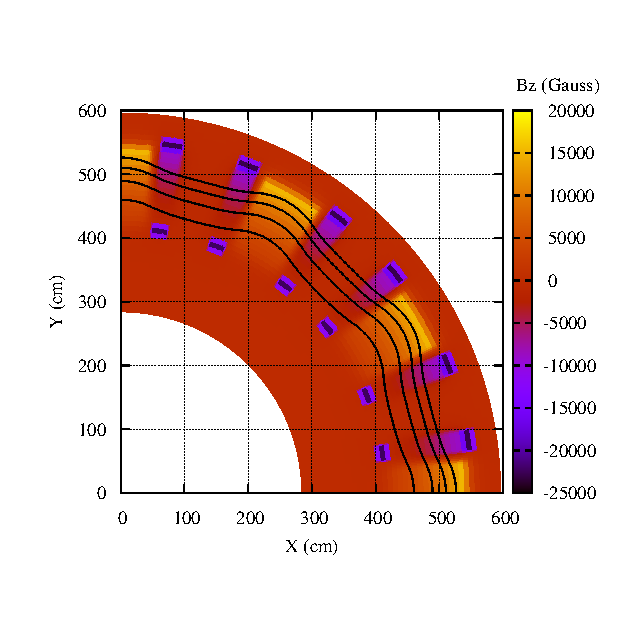
\includegraphics[width=.8\linewidth]{./figs_FFAG_introSlides/Quadrant.eps}
\end{minipage}\hspace{0mm}
\begin{minipage}{.499\linewidth}
%\centering 
\blue
\underline{H and V tunes constant} \\[0ex]
 \includegraphics*[bbllx=20,bblly=90,bburx=567,bbury=457,width=.7\linewidth]{./figs_FFAG_introSlides/tuneDiag_50traj.eps}
\end{minipage}\hspace{0mm}


\end{minipage}\hspace{0mm}



\end{minipage}








\clearpage 

\large 

\subsection*{\LARGE \nib  Basic theory}

\subsection*{\LARGE \blue \nid  Combined function optics}


\large 


{\centering

\nib A  rule that  yields the orientation of $\vec F$~: 

{\blue \nib\  $I\vec{dl}$ , $\vec B$ and $\vec F$, in that order, form a direct triedra }
%\hspace{60mm}
%\raisebox{-10mm}[0mm][0mm]{\includegraphics*[bbllx=0,bblly=0,bburx=300,bbury=254,width=4cm]{./figs_FFAG_introSlides/fFoc.eps}\hspace{-5mm}}
%~     ~ ~ ~ ~ ~ ~ ~ 

~


\mbox{
\begin{minipage}[b]{.5\linewidth}\hspace{3mm}
%\begin{center}
\includegraphics*[bbllx=34,bblly=70,bburx=245,bbury=220,width=12cm]{./figs_FFAG_introSlides/ring1Draw.eps}

~

~

%\hspace{2cm}\includegraphics*[bbllx=14,bblly=14,bburx=278,bbury=260,width=10cm, height=5cm]{./figs_FFAG_introSlides/fieldMarkI.eps}
\end{minipage}
\begin{minipage}[b]{.5\linewidth}\hspace{3mm}

\mbox{
\includegraphics*[bbllx=0,bblly=100,bburx=252,bbury=323,width=7cm]{./figs_FFAG_introSlides/geometry.eps}\hspace{-5mm}
\includegraphics*[bbllx=0,bblly=100,bburx=252,bbury=323,width=7cm]{./figs_FFAG_introSlides/geometryD.eps} 
}

~

~


\mbox{\hspace{3mm}
\includegraphics*[bbllx=0,bblly=0,bburx=300,bbury=254,width=6cm]{./figs_FFAG_introSlides/fFoc.eps}  \hspace{5mm}
\includegraphics*[bbllx=0,bblly=0,bburx=300,bbury=254,width=6cm]{./figs_FFAG_introSlides/dFoc.eps}
}

(in this sketch I assume field obtained from pole shaping, just for simplicity)
%\end{center}


\end{minipage}
}

}%\centering







\clearpage 

{\fontsize{17}{25} \selectfont

\subsubsection*{\LARGE \nib Solution of the motion across a combined function magnet \label{slideODE}}


\nid A reference trajectory can be defined, characterized by $B_0 \rho_0 = \frac{ \textstyle{p_0}}{\textstyle{q}}$ 

\nid The equations of small amplitude motion $(x = \rho - \rho_0, y)$ of a particle,  in the Serret-Frenet frame 
attached to that reference curve, are  derived from the Lorentz force equation 
$$ \frac{ \textstyle{d\vec p}}{\textstyle{d t}} = q \vec v \times \vec B$$

\nin using a  transverse expansion of the magnetic field $\vec B(s)$ along the trajectory~: 

$B_x = -n \frac{\textstyle{B_0}}{\textstyle{\rho_0}} y  ~ ~ \textsl{ [ + non-linear terms]}$, ~ ~ ~
$B_y = B_0 (1-n \frac{\textstyle{x}}{\textstyle{\rho_0}} )   ~ ~ \textsl{  [ + non-linear terms]}$ \\
\\
\begin{minipage}[b]{.6\linewidth}

\nid In expanding $\vec B$  the field index has been  introduced~:
$$n = -\frac{\textstyle{\rho_0}}{\textstyle{B_0}}   \frac{\textstyle{\partial B}}{\textstyle{\partial x}}  $$

The FFAG index $K=\frac{\textstyle{r}}{\textstyle{B}}   \frac{\textstyle{\partial B}}{\textstyle{\partial r}}$  {(of  $B = B_0 (\frac{r}{r_0})^K$ )} relates to 

%\medskip
%{  $   \frac{dB}{dr} = K \frac{B_0}{r_0}  (\frac{r}{r_0})^{K-1}  = K \frac{B }{ R} 
%~~~~$} \textsf{so that} {  $~~~~ \frac{r}{B} \frac{dB}{dr} =$ 
$n$ by \centering{\fbox{$ K \approx -n r/\rho$}. }



~

\nid Calculations (found in text books) lead to the linear approximation~: \\[-2ex]
{\blue \LARGE 
$$ \left| 
\begin{array}{lr} 
\frac{\textstyle{d^2x}}{\textstyle{ds^2}} + \frac{\textstyle{1 - n}}{\textstyle{\rho_0^2}}  \, x =   
\frac{\textstyle{1}}{\textstyle{\rho_0}} \frac{\textstyle{\Delta p}}{\textstyle{p}} \\
\frac{\textstyle{d^2y}}{\textstyle{ds^2}} + \frac{\textstyle{ n}}{\textstyle{\rho_0^2}}  \, y =   0
\end{array} 
\right. $$
}

\end{minipage}\hspace{15mm}
\begin{minipage}[b]{.19\linewidth}

\mbox{
\includegraphics*[bbllx=0,bblly=100,bburx=252,bbury=323,width=1.1\linewidth]{./figs_FFAG_introSlides/geometry.eps}\hspace{5mm}
%\includegraphics*[bbllx=0,bblly=100,bburx=252,bbury=323,width=.99\linewidth]{./figs_FFAG_introSlides/geometryD.eps} 
}


~


\mbox{\hspace{3mm}
\includegraphics*[bbllx=0,bblly=0,bburx=300,bbury=254,width=1.1\linewidth]{./figs_FFAG_introSlides/fFoc.eps}  \hspace{5mm}
%\includegraphics*[bbllx=0,bblly=0,bburx=300,bbury=254,width=.9\linewidth]{./figs_FFAG_introSlides/dFoc.eps}
}


\end{minipage}

} %fontsize


\clearpage



{\blue 

\fontsize{30}{36} \selectfont

\nib HOME WORK  : 

~

~

What  approximation leads to  ~ ~ $ K \approx -n R/\rho$ ?

}



\clearpage 

{\fontsize{20}{28} \selectfont

\nid Solving these two differential equations yields  the coordinates across a magnet

  (with $\mathcal{L}=(s-s_0)$ being the path length along the trajectory arc)~: 


{\blue \bf \underline{Radial motion}}

\medskip
\fcolorbox{white}{blue!10!white}{\underline{if $(1-n)>0$~:  }}

$~ \left| 
\begin{array}{l} 
 x = x_0 \cos\frac{\textstyle{\sqrt{1-n}}}{\textstyle{\rho_0}} \mathcal{L} + \frac{\textstyle{x'_0}}{\textstyle{\frac{\textstyle{\sqrt{1-n}}}{\textstyle{\rho_0}}}}  \sin\frac{\textstyle{\sqrt{1-n}}}{\textstyle{\rho_0}}  \mathcal{L}  
 + \frac{\textstyle{\rho_0}}{\textstyle{\sqrt{1-n}}}(1 - \cos\frac{\textstyle{\sqrt{1-n}}}{\textstyle{\rho_0}} \mathcal{L} )
\ \frac{\textstyle{\Delta p}}{\textstyle{p}} \\
 x' = -x_0 \frac{\textstyle{\sqrt{1-n}}}{\textstyle{\rho_0}} \sin\frac{\textstyle{\sqrt{1-n}}}{\textstyle{\rho_0}}  \mathcal{L} + x'_0  \cos\frac{\textstyle{\sqrt{1-n}}}{\textstyle{\rho_0}}  \mathcal{L} 
 + \frac{\textstyle{\rho_0}}{\textstyle{\sqrt{1-n}}}\sin\frac{\textstyle{\sqrt{1-n}}}{\textstyle{\rho_0}} \mathcal{L} 
\ \frac{\textstyle{\Delta p}}{\textstyle{p}}\\
\end{array} \right.$

~

\fcolorbox{white}{blue!10!white}{\underline{if $(1-n)<0$~: }}

$ \left| 
\begin{array}{l} 
 x = x_0 \cosh\frac{\textstyle{\sqrt{n-1}}}{\textstyle{\rho_0}} \mathcal{L} + \frac{\textstyle{x'_0}}{\textstyle{\frac{\textstyle{\sqrt{n-1}}}{\textstyle{\rho_0}}}}  \sinh\frac{\textstyle{\sqrt{n-1}}}{\textstyle{\rho_0}}  \mathcal{L}  
 + \frac{\textstyle{\rho_0}}{\textstyle{n-1}}(1 - \cosh\frac{\textstyle{\sqrt{n-1}}}{\textstyle{\rho_0}} \mathcal{L} )
\ \frac{\textstyle{\Delta p}}{\textstyle{p}}\\
 x' = x_0 \frac{\textstyle{\sqrt{n-1}}}{\textstyle{\rho_0}} \sinh\frac{\textstyle{\sqrt{n-1}}}{\textstyle{\rho_0}}  \mathcal{L} + x'_0  \cosh\frac{\textstyle{\sqrt{n-1}}}{\textstyle{\rho_0}}  \mathcal{L} 
 + \frac{\textstyle{\rho_0}}{\textstyle{n-1}}\sinh\frac{\textstyle{\sqrt{n-1}}}{\textstyle{\rho_0}} \mathcal{L} 
\ \frac{\textstyle{\Delta p}}{\textstyle{p}}\\
\end{array} \right.$

~


{\blue \bf  \underline{Axial motion~: }}

\medskip

\begin{minipage}{0.49\linewidth}
\fcolorbox{white}{blue!10!white}{\underline{if $n>0$~:  }}


$~ \left| 
\begin{array}{l} 
 y = y_0 \cos\frac{\textstyle{\sqrt{n}}}{\textstyle{\rho_0}}  \mathcal{L} + \frac{\textstyle{y'_0}}{\textstyle{\frac{\textstyle{\sqrt{n}}}{\textstyle{\rho_0}}}}  \sin\frac{\textstyle{\sqrt{n}}}{\textstyle{\rho_0}}  \mathcal{L}  \\
 y' = -y_0 \frac{\textstyle{\sqrt{n}}}{\textstyle{\rho_0}} \sin\frac{\textstyle{\sqrt{n}}}{\textstyle{\rho_0}}  \mathcal{L} + y'_0  \cos\frac{\textstyle{\sqrt{n}}}{\textstyle{\rho_0}}  \mathcal{L} \\
\end{array} \right.$

~


\end{minipage}
\begin{minipage}{0.49\linewidth}
\fcolorbox{white}{blue!10!white}{\underline{if $n<0$~: }}


$ \left| 
\begin{array}{l} 
 y = y_0 \cosh\frac{\textstyle{\sqrt{-n}}}{\textstyle{\rho_0}} \mathcal{L} + \frac{\textstyle{y'_0}}{\textstyle{\frac{\textstyle{\sqrt{-n}}}{\textstyle{\rho_0}}}}  \sinh\frac{\textstyle{\sqrt{-n}}}{\textstyle{\rho_0}}  \mathcal{L} \\ 
 y' = y_0 \frac{\textstyle{\sqrt{-n}}}{\textstyle{\rho_0}} \sinh\frac{\textstyle{\sqrt{-n}}}{\textstyle{\rho_0}}  \mathcal{L} + y'_0  \cosh\frac{\textstyle{\sqrt{-n}}}{\textstyle{\rho_0}}  \mathcal{L} \\
\end{array} \right.$

\end{minipage}

}





\clearpage 

{\fontsize{16}{20} \selectfont

\subsection*{\LARGE  \nid In transport matrix notations  (with, for short, 
$k_x = |1-n| /\rho_0^2, ~ ~ ~ k_y = |n| /\rho_0^2$)}


\fcolorbox{white}{blue!10!white}{\underline{If $n < 0$~:}  The dipole is horizontally focusing and vertically defocusing}
{%\large
$$\left(
\begin{array}{ccccc} x \\ x' \\ y \\ y' \\ \frac{\textstyle{\delta p}}{\textstyle{p}} 
\end{array} 
\right)
\! = \!
\left(
\begin{array}{ccccc} 
 \cos \sqrt{k_x} \mathcal{L} & \frac{\textstyle{1}}{\textstyle{\sqrt{k_x}}}  \sin \sqrt{k_x}  \mathcal{L}  
 & 0& 0 & \frac{\textstyle{1}}{\textstyle{\rho k_x}}(1 - \cos \sqrt{k_x} \mathcal{L} ) \\[-.4000ex]
 - \sqrt{k_x} \sin \sqrt{k_x}  \mathcal{L} 
&   \cos \sqrt{k_x}  \mathcal{L} 
 & 0 & 0 & \frac{\textstyle{1}}{\textstyle{\rho \sqrt{k_x}}}\sin \sqrt{k_x} \mathcal{L} \\[-.4000ex]
0 & 0 &  \cosh \sqrt{k_y} \mathcal{L} & \frac{\textstyle{1}}{\textstyle{ \sqrt{k_y}}}  \sinh \sqrt{k_y}  \mathcal{L} & 0 \\ [-.4000ex]
0 & 0 &  \sqrt{k_y} \sinh \sqrt{k_y}  \mathcal{L} &  \cosh \sqrt{k_y}  \mathcal{L} & 0  \\[-.4000ex]
0 & 0 & 0 & 0 & 1 
\end{array} \right)
\left(
\begin{array}{ccccc} x_0 \\ x'_0 \\ y_0  \\ y'_0  \\  \frac{\textstyle{\delta p}}{\textstyle{p}} 
\end{array} 
\right)$$
}

\fcolorbox{white}{blue!10!white}{\underline{If $ 0 < n < 1$~:  }
The dipole is focusing in both planes. aka ``weak focusing'' } (cyclotrons)
{%\large
$$\left(
\begin{array}{ccccc} x \\ x' \\ y \\ y' \\ \frac{\textstyle{\delta p}}{\textstyle{p}} 
\end{array} 
\right)
\! = \!
\left(
\begin{array}{ccccc} 
 \cos \sqrt{k_x} \mathcal{L} & \frac{\textstyle{1}}{\textstyle{\sqrt{k_x}}}  \sin \sqrt{k_x}  \mathcal{L}  
 & 0& 0 & \frac{\textstyle{1}}{\textstyle{\rho k_x}}(1 - \cos \sqrt{k_x} \mathcal{L} ) \\[-.4000ex]
 - \sqrt{k_x} \sin \sqrt{k_x}  \mathcal{L} 
&   \cos \sqrt{k_x}  \mathcal{L} 
 & 0 & 0 & \frac{\textstyle{1}}{\textstyle{\rho \sqrt{k_x}}}\sin \sqrt{k_x} \mathcal{L} \\[-.4000ex]
0 & 0 &  \cos \sqrt{k_y} \mathcal{L} & \frac{\textstyle{1}}{\textstyle{ \sqrt{k_y}}}  \sin \sqrt{k_y}  \mathcal{L} & 0 \\ [-.4000ex]
0 & 0 &  -\sqrt{k_y} \sin \sqrt{k_y}  \mathcal{L} &  \cos \sqrt{k_y}  \mathcal{L} & 0  \\[-.4000ex]
0 & 0 & 0 & 0 & 1 
\end{array} \right)
\left(
\begin{array}{ccccc} x_0 \\ x'_0 \\ y_0  \\ y'_0  \\ \frac{\textstyle{\delta p}}{\textstyle{p}} 
\end{array} 
\right)$$
}


\fcolorbox{white}{blue!10!white}{\underline{If $n > 1$~:  }
The dipole is horizontally defocusing and vertically focusing.} 
{%\large
$$\left(
\begin{array}{ccccc} x \\ x' \\ y \\ y' \\ \frac{\textstyle{\delta p}}{\textstyle{p}} 
\end{array} 
\right)
\! = \!
\left(
\begin{array}{ccccc} 
 \cosh \sqrt{k_x} \mathcal{L} & \frac{\textstyle{1}}{\textstyle{\sqrt{k_x}}}  \sinh \sqrt{k_x}  \mathcal{L}  
 & 0& 0 & \frac{\textstyle{1}}{\textstyle{\rho k_x}}(1 - \cosh \sqrt{k_x} \mathcal{L} ) \\[-.4000ex]
 \sqrt{k_x} \sinh \sqrt{k_x}  \mathcal{L} 
&   \cosh \sqrt{k_x}  \mathcal{L} 
 & 0 & 0 & \frac{\textstyle{1}}{\textstyle{\rho \sqrt{k_x}}}\sinh \sqrt{k_x} \mathcal{L} \\[-.4000ex]
0 & 0 &  \cos \sqrt{k_y} \mathcal{L} & \frac{\textstyle{1}}{\textstyle{ \sqrt{k_y}}}  \sin \sqrt{k_y}  \mathcal{L} & 0 \\ [-.4000ex]
0 & 0 &  -\sqrt{k_y} \sin \sqrt{k_y}  \mathcal{L} &  \cos \sqrt{k_y}  \mathcal{L} & 0  \\[-.4000ex]
0 & 0 & 0 & 0 & 1 
\end{array} \right)
\left(
\begin{array}{ccccc} x_0 \\ x'_0 \\ y_0  \\ y'_0  \\ \frac{\textstyle{\delta p}}{\textstyle{p}} 
\end{array} 
\right)$$
}




\clearpage 

\subsection*{\LARGE \nid ``MARK I'' uses strong focusing,  BF is focusing, BD is defocusing }


\nib\ The (BF,BD) doublet is globally  focusing  in both  $x$ and $y$ planes~: 

~

\begin{center}
\includegraphics*[width=0.9\linewidth]{./figs_FFAG_introSlides/focAlternee.eps}
\end{center}

}







\clearpage 



{\LARGE \bf \nid Wedge focusing is required to complete the (BF,BD) cell matrix}


{\Large - It stems from the orbit geometry~:}


\begin{center}
\includegraphics*[width=0.5\linewidth]{./figs_FFAG_introSlides/mura043_wedgeFoc.eps}

K.R. Symon, The FFAG synchrotron MARK I, MURA-KRS-6 (1954) 
\end{center}



\clearpage 

{\fontsize{17}{30} \selectfont

\subsection*{\LARGE \nid MARK I is a ring, one more ingredient is needed to make it operational~: \\ periodic stability}

\nib Let's oversimplify~: we forget drifts, wedge focusing, 



\nib let's also consider  magnets with same field ($B_{\rm 0,F}=B_{\rm 0,D}$) and same index ($k_F = k_D = k$), 



\nib thus the transport matrix for the  (BF,BD) cell writes~:



$$
\left(
\begin{array}{cc} 
 \cosh \sqrt{k_D} \mathcal{L_D} & \frac{\textstyle{1}}{\textstyle{\sqrt{k_D}}}  \sinh \sqrt{k_D}  \mathcal{L_D}   \\[-.4000ex]
 \sqrt{k_D} \sinh \sqrt{k_D}  \mathcal{L_D} &   \cosh \sqrt{k_D}  \mathcal{L_D}  \\[-.4000ex]
\end{array} \right)
\times
\left(
\begin{array}{cc} 
 \cos \sqrt{k_F} \mathcal{L_F} & \frac{\textstyle{1}}{\textstyle{\sqrt{k_F}}}  \sin \sqrt{k_F}  \mathcal{L_F}   \\[-.4000ex]
 -\sqrt{k_F} \sin \sqrt{k_F}  \mathcal{L_F} &   \cos \sqrt{k_F}  \mathcal{L_F}  \\[-.4000ex]
\end{array} \right)
=
$$



$$
\left(
\begin{array}{cc} 
 \cosh \sqrt{k} \mathcal{L_D} \times  \cos \sqrt{k} \mathcal{L_F} -  \sinh \sqrt{k}  \mathcal{L_D} \times \sin \sqrt{k}  \mathcal{L_F}& (*)   \\[-.4000ex]
 (*) &  \sinh \sqrt{k} \mathcal{L_D}\times  \sin \sqrt{k}  \mathcal{L_F} +   \cosh \sqrt{k}  \mathcal{L_D}\times  \cos \sqrt{k}  \mathcal{L_F}  \\[-.4000ex]
\end{array} \right)
$$

~

\nib Periodic stability requires 

$$\rm \frac{\textstyle{1}}{\textstyle{2}} Trace[Cell Matrix] < 1 \ \ \ \ \ \ - \textrm{for both planes !}$$

\ie,

{\blue \LARGE
$$  \cosh \sqrt{k} \mathcal{L}_D \times  \cos \sqrt{k} \mathcal{L}_F <1 \ \ \ \textrm{and} \ \ \  \cos \sqrt{k} \mathcal{L}_D \times  \cosh \sqrt{k} \mathcal{L}_F <1 \ \ \ \  (\textrm{noting} \  \sqrt{k} \mathcal{L} = \sqrt{k}\mathcal{L})$$
}


}%fontsize


\clearpage



{\blue 

\fontsize{30}{36} \selectfont

\nib HOME WORK  : 

~

~


\nin Plot the stability diagram, \ie, the region of periodic stability 
in the  $(\sqrt{k} \mathcal{L}_F,  \sqrt{k} \mathcal{L}_D)$ space (take $\sqrt{k} \mathcal{L}_F\in[0, 2\pi]$, $  \sqrt{k} \mathcal{L}_D\in [0,2\pi]$).
}







\clearpage


{\fontsize{18}{28} \selectfont

\subsection*{\LARGE \nib  Constant tunes}


\nid Re-write the linearized equation of motion (slide \#\ref{slideODE})
with  the transformation $s = r \, \theta $  yields 
\begin{eqnarray}
& \frac{\textstyle{d^2x}}{\textstyle{d\theta^2}} + \left(\frac{\textstyle{r(\theta)^2}}{\textstyle{\rho^2(r,\theta)}}\left[1-n\right]\right) x = 0 \label{eq_motion2} \vspace{2mm} \nonumber \\
& \frac{\textstyle{d^2y}}{\textstyle{d\theta^2}} + \left(\frac{\textstyle{r(\theta)^2}}{\textstyle{\rho^2(r,\theta)}} n \right) y = 0 \nonumber 
\end{eqnarray}  \\
(r is the local radius of the trajectory wrt center of the ring, $\rho$ is the local curvature radius).


\nid Thus, two sufficient conditions to have both the vertical and horizontal betatron oscillations constant with respect to the momentum
(\ie, the forcing terms in the above equations constant), are:
\begin{eqnarray}
\left. \frac{\partial n}{\partial p} \right|_{\theta=const} = 0  \label{card1} \nonumber \\
\left. \frac{\partial}{\partial p}\left(\frac{r}{\rho}\right) \right|_{\theta=const} = 0 \label{card2}  \nonumber 
\end{eqnarray}

- the first one expresses the constancy of the field index with respect to the momentum 

- the second one expresses the similarity of the closed orbits. 

~

\nin This defines a ``zero-chromaticity''  optics~: \begin{eqnarray}  \frac{\delta \nu }{ \delta p/p}=0 \end{eqnarray}
}




\clearpage

{\blue 

\fontsize{30}{36} \selectfont

\nib HOME WORK : 

~

~

\nin Show that, with the FFAG scaling law $B=B_0 (r/r_0)^K \, \mathcal{F}(\theta)$, 
this happens.

(take a step function for $\mathcal{F}(\theta)$~: 1 inside the magnets, 0 outside)
}

\clearpage


{\fontsize{18}{34} \selectfont

\subsection*{\LARGE \nib  Longitudinal motion, longitudinal stability}



\nid  If  synchrotron style of RF operation is used, then the \\
longitudinal motion satisfies the regular phase-stability principles, 

\medskip
{\Large ~ ~ ~ ~ ~ ~ ~ ~ ~ ~ ~ ~ ~ ~ ~  ~ ~ ~ ~ ~ ~ ~  %\fbox{ 
$ \Phi'' + \frac{\Omega^2}{\cos{\phi_s}}(\sin\phi - \sin \phi_s)=0$}
~ ~ ~ ~ ~ ~ ~ ~ ~ ~ ~ ~ 
\raisebox{-3mm}[0mm][0mm]{\includegraphics*[bbllx=20,bblly=100,bburx=560,bbury=460,width=7cm]{./figs_FFAG_introSlides/synMot100MeV.eps}}

\medskip
\nin synchrotron frequency {\Large $f_s = \Omega_s/2\pi = \frac{c}{\mathcal{L}}\left( 
\frac{h \eta  \cos\phi_s q\hat{V}}{2 \pi E_s}\right)^{1/2}$~, } 
%, given $h=1$, $\phi_s=0$, $q\hat{V}=0.019$~MeV~; 
%$E_s$ is total energy and $T_{rev}$ and $\mathcal{L}$ are obtained by tracking (Tab.~\ref{TabParam150}),  
 bucket height  {\Large $\pm \frac{\Delta p}{p} = \pm \frac{1}{\beta_s} 
\left(\frac{ 2 q\hat{V}}{\pi h \eta E_s}\right)^{1/2}$ ,}      ~~  etc.



%``By virtue of its essential simplicity, the reversed-field type FFAG may remain of interest for 
%accelerators of low or intermediate energy, especially if a high duty-factor can be efficiently realized \[...\]''


\subsection*{\LARGE \nib Betatron damping}

Introducing the velocity term and its variation, the previous differential \\[0ex]
\mbox{
\begin{minipage}[b]{.59\linewidth}
equations change to~: 
{\blue \Large 
$ \left| 
\begin{array}{lr} 
x'' + \frac{\textstyle{{(\beta \gamma})'}}{\textstyle{\beta \gamma}} x' + \frac{\textstyle{1 - n}}{\textstyle{\rho_0^2}}  \, x =   
\frac{\textstyle{1}}{\textstyle{\rho_0}} \frac{\textstyle{\Delta p}}{\textstyle{p}} \\
y'' + \frac{\textstyle{{(\beta \gamma})'}}{\textstyle{\beta \gamma}} y' + \frac{\textstyle{n}}{\textstyle{\rho_0^2}}  \, y =0   
\end{array} 
\right. $
}

~

Solving (text books ...) yields (same for y, y') \\[0ex]
$x \propto \sqrt{ \frac{\textstyle{r}}{\textstyle{\beta \gamma}}}$, ~ ~ $x' \propto \sqrt{ \frac{\textstyle{1}}{\textstyle{r \times \beta \gamma}}}$
\end{minipage}\hspace{0mm}
\begin{minipage}[b]{.39\linewidth}
 \includegraphics*[width=1.15\linewidth]{./figs_FFAG_introSlides/dampZZp.eps}
\end{minipage}\hspace{0mm}
}

}%fontsize






%\clearpage 

\hspace{-3ex}
\begin{minipage}[b]{1.\linewidth}
{\fontsize{16}{19} \selectfont


\subsection*{\LARGE \nib  Second model, spiral sector FFAG, ``MARK V''}

\nid The idea in the spiral FFAG was to 
avoid the ``wrong sign''  curvature and bring the circumference factor $C = R/\rho$ close to 1.
The  wedge angles provides the vertical focusing. 

\nid R\&D objectives~:  spiral FFAG POP - first extensive use of computers to determine 
magnetic field  and machine  parameters~; long-term orbit stability~; RF acceleration methods. \\
\\[-0ex]
\begin{minipage}[b]{.3\linewidth}
\centering

\includegraphics*[bbllx=14,bblly=44,bburx=250,bbury=230,width=6.cm,height=3.cm]{./figs_FFAG_introSlides/ringSpiralMagDraw.eps}

 Spiral dipole, $B>0$, H-focusing \\[-1ex]
scaling gap g$\propto$r\\[1ex]
%\hspace{-7mm} \includegraphics*[width=9.cm]{./figs_FFAG_introSlides/spiralFFAG.eps}
 \includegraphics*[width=.99\linewidth]{./figs_FFAG_introSlides/markv.eps}

%\smallskip

%\includegraphics*[bbllx=14,bblly=44,bburx=278,bbury=195,width=5.5cm]{./figs_FFAG_introSlides/ringSpiralCoilDraw.eps}

 \includegraphics*[angle=90,width=.99\linewidth]{./figs_FFAG_introSlides/markV_tuneDiag.eps}

~~~~~~~~~~~~~~~~

~~~~~~~~~~~~~~~~

~~~~~~~~~~~~~~~~



\end{minipage}\hspace{0mm}
\begin{minipage}[b]{.63\linewidth}
\Large   

\vspace{-0ex}
  \begin{center}
   \begin{tabular}{llccc}
\multicolumn{5}{c}{\blue \bf \Large
First operation Aug.~1957 at the  MURA Lab., Madison. } \\[1ex]
\multicolumn{4}{c}{\bf MARK V PARAMETERS}    &     \bf     \\[2mm]
&$E_{inj} - E_{max}$&\it keV &    35 - 180      & \bigg\{ \raisebox{1ex}[0mm][0mm]{\it reasonable size}  \\
      &             &     &                  &  \raisebox{2ex}[0mm][0mm]{\it  magnets}   \\[-2ex]
      &orbit radius &\it  m   &   0.34 - 0.52   &  \normalsize \bf spiraling orbit    \\
      &$E_{tr}~/~r_{tr}$&\it keV~/~m&   155~/~0.49      &  \bigg\{ \raisebox{1ex}[0mm][0mm]{\it RF exprmnts ~~~~ ~ ~ ~~~ } \\
      &                &  &                  &   \raisebox{2ex}[0mm][0mm]{\it  at  $\gamma_{tr} =(1+K)^{1/2}$ }     \\[-2ex]
\\[-2.0ex]
\multicolumn{2}{l}{\it \underline{Optics}}  & \multicolumn{3}{l}{ \bf strong focusing, ~ scaling}   \\
      & lattice    &     &    N  spiral sectors  &   \\
      & number of sectors& &       6           &  \\[-.5ex]
      & field index $K$&  &      0.7          &   \bigg\{ \raisebox{1ex}[0mm][0mm]{\it coil windings, }  \\
      &                &  &                   &    \raisebox{2ex}[0mm][0mm]{\it  ~ ~ ~ ~ tunable 0.2-1.16  }       \\[-2ex]
      & flutter $F_{eff}$ &     &       1.1          &  \it tuning coils / 0.57 - 1.60 \\
      &$\nu_r~/~\nu_z$&  &   1.4~/~1.2       &  \it tunable  \\
      &$\beta_r ~/~ \beta_z$&\it m  &   0.45-1.3~/~0.6-1.4       &   \it  min-max  \\
\\[-2.0ex]
\multicolumn{2}{l}{\it \underline{Magnet}}& \multicolumn{3}{l}{\bf spiral sector, $B=B_0 (\frac{r}{r_0})^K \, \mathcal{F}(N(\tan \zeta \ln \frac{r}{r_0} -  \theta))$} \\
%      &  $1/w$       &     &       6.25          &   \it $2 \pi w r_0\approx$ ridges radial separation \\
      &  $\zeta$ &\it deg&  46       &  \it edge to radius angle  \\
%      &  $r_{min} - r_{max}$&\it m&    0.25 - 0.61  &  \\
      &   gap      &\it cm  &      16.5  - 7     &   \it $g/r=$Cte  \\
\\[-1.50ex]
\multicolumn{2}{l}{\it  \underline{Injection}}&   &cont. or pulsed &  \it e-gun + e-inflector \\
\\[-1.50ex]
\multicolumn{2}{l}{\it  \underline{Acceleration}}&&    \sf betatron and RF   & \it extensive RF tests   \\
%      & RF  voltage&\it V  &        150         &  \\
   \end{tabular}
  \end{center}

~~~~~~~~~~~~~~~

~~~~~~~~~~~~~~~

~~~~~~~~~~~~~~~

~~~~~~~~~~~~~~~

~~~~~~~~~~~~~~~

\end{minipage}

}
\end{minipage}




%\clearpage 


\begin{minipage}[b]{1.\linewidth}

\subsection*{\LARGE \nib  On the optics  in the spiral FFAG }

 \sf 
\fontsize{19}{24} \selectfont

\nid The following form for the field preserves the scaling property in an N-periodic  spiral FFAG: \\
{\LARGE \blue  $   B(r, \theta)|_{z=0} = B_0 \left( \frac{r}{r_0} \right)^K \ 
\mathcal{F}\left(N( \tan \zeta \times \ln \frac{r}{r_0} - \theta) \right) $} \\
\begin{minipage}[b]{.7\linewidth}

\fontsize{18}{23} \selectfont

%\large \sf 

$\mathcal{F}$ is the axial modulation of the field (``flutter''). One can for instance think of \\
{\blue $\mathcal{F}=1+f\sin\left( N(\tan \zeta \ln \frac{r}{r_0} -  \theta) \right)$, $f\approx 0.25$. }

\medskip
- The logarithmic spiral edge { \blue ($r = r_0 \exp((\theta-\theta_0)/\tan \zeta$) }
 ensures constant  angle between  spiral sector edges and radius.

- The in and out wedge angles  are different,  V-defocusing, 
and V-focusing (larger), overall effect is vertical focusing.

%\medskip
%The modulation is $2\pi/N$-periodic, a particle passes N ridges over a turn. 


\medskip

\nid Effect field fall-off extent on vertical focusing\\[1ex]
$ 
\left( \begin{array}{c}
 x \\ x' 
\end{array} \right)
=
\left(  \begin{array}{cc}
1 & 0 \\
\frac{\tan \epsilon}{\rho} & 1
\end{array}  \right)
\left( \begin{array}{c}
 x_0 \\ x_0' 
\end{array} \right)
$, 
$ 
\left( \begin{array}{c}
 y \\ y' 
\end{array} \right)
=
\left(  \begin{array}{cc}
1 & 0 \\
-\frac{\tan(\epsilon -\psi)}{\rho} & 1
\end{array}  \right)
\left( \begin{array}{c}
 y_0 \\ y_0' 
\end{array} \right)
$, \\[1ex]
where $\psi=\frac{I_1\cdot\lambda\cdot(1+sin^2(\epsilon))}{\rho\cdot cos(\epsilon)}$, 
with
$ I_1=\int \frac{B_z(s)\cdot(B_0-B_z(s))}{\lambda\cdot B_0^2}\cdot ds $, 
$\lambda$ is the fringe field extent. 




\medskip
%In a simpler hard-edge model, 
%the optical ingredients to describe the closed orbit would be  the sector angle $\theta$ between edges, arc length $s$ and 
%curvature radius $\rho$,  the  index $n=-K\rho/R$ provides  
%the $\left( \begin{array}{cc} C & S \\ C' & S'\end{array} \right)$ matrix, 
%the wedge angle $\epsilon$ provides  the wedge matrices. 

%The half trace of the resulting product matrix yields

\nid Expansion of the equations of motion around the scalloped orbit in the linear approximation  yields the 
approximate tunes 
 $$\nu_r \approx \sqrt{1 + K} , ~ ~ ~  \nu_z \approx  \sqrt{-K + F^2 (1 + 2\tan^2 \zeta)} \ \ \ 
(F = \frac{\overline{B^2}}{\overline{B}^2} - 1 ~  \stackrel{hard-edge}{-\!\!\!-\!\!\!\longrightarrow} ~ \frac{R}{\rho} -1)$$

%A matrix model using hard-edge approximation would give similar result to first order in the deviation. 

~

~


\end{minipage}\hspace{5mm}
\begin{minipage}[b]{.3\linewidth}

\includegraphics[bbllx=90,bblly=0,bburx=500,bbury=460,width=.99\linewidth]{./figs_FFAG_introSlides/spiral3D.eps}

%\vspace{-20mm}
%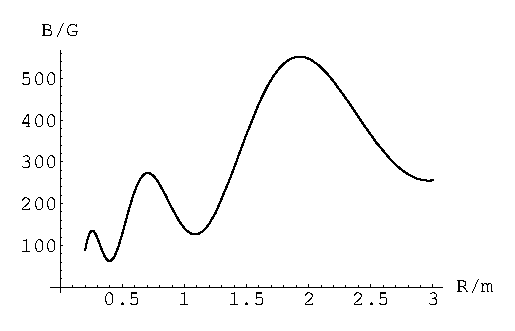
\includegraphics[width=.9\linewidth]{./figs_FFAG_introSlides/spiralBvsR.eps}

\vspace{-0mm}
 \hspace{10mm}\includegraphics*[bbllx=14,bblly=120,bburx=520,bbury=500,width=.99\linewidth]{./figs_FFAG_introSlides/spiralFoc.eps}

~

~

\end{minipage}
\end{minipage}





\clearpage 

{\fontsize{17}{20} \selectfont

\subsection*{\LARGE  \nib Second radial sector, 50~MeV,  2-way}


\nid Preliminary studies early 1957. The spiral sector e-model was not yet completed - this determined the choice of radial sector~:  
easier to design, better understood.  Pole is not scaling~: $g\propto 1/r$, constant tunes require tweaking the flutter, and pole face windings.

\nid Study objectives~: ~~ RF stacking, ~ high circulating $I$, ~ 2-way storage. 

\nid First start Dec.~1959, 2-beam mode, 27~MeV~; disassembled in 60, magnets corrected~;  second start Aug.~61, single beam, 50~MeV. \\[-2ex]
\begin{minipage}[b]{.38\linewidth}
\centering

%\hspace{-10mm} 
\includegraphics*[width=.95\linewidth]{./figs_FFAG_introSlides/2wayFFAG.eps} 
%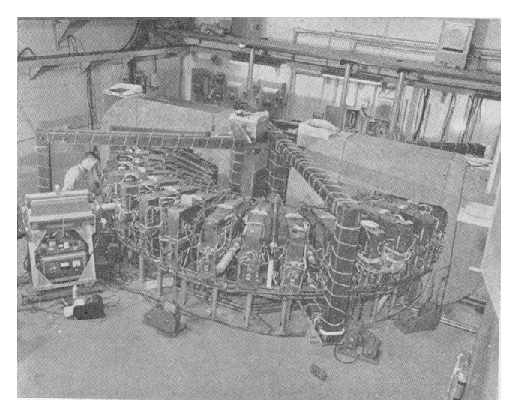
\includegraphics[width=16.cm]{./figs_FFAG_introSlides/photoRing.eps}

%\vspace{-30mm}
\includegraphics*[width=.6\linewidth]{./figs_FFAG_introSlides/ring3Draw.eps} 

\end{minipage}\hspace{0mm}
\begin{minipage}[b]{.65\linewidth}
\large   
  \begin{center}
   \begin{tabular}{llccc}
\\[-3mm]
\multicolumn{4}{c}{\bf FFAG parameters}    &     \\[2mm]
      & \bf $E_{inj} - E_{max}$  & \it     MeV  & \bf    0.1 - 50     & \bf     \it reasonable size \& beam life-time         \\
      & \bf orbit radius& \it  m   & \bf     1.20 - 2.00    & $\ B\rho\ : 0.001 \rightarrow 0.17$ (T.m)    \\    \\[0ex]
\multicolumn{2}{l}{\it \underline{Optics}}   \\
      & \bf  lattice    &       & \bf    FODO            & \it $B\approx B_0(r/r_0)^K\, \cos(16\, \theta)$    \\
      & \bf  number of cells&   & \bf      16            & \bf      \it 32 magnets, 3.15~deg. drifts     \\
      & \bf    K        &       & \bf       9.25         & \bf             \\
      & \bf $\nu_r~/~\nu_z$&    & \bf     4.42~/~2.75    & \bf         \\[.5ex]
%      & \bf  radial accept. & \bf  $\pi$cm & \bf    0.4    & \bf   \raisebox{1ex}[0mm][0mm]{\it mechanical limit is}  \\
%      & \bf             & \bf      & \bf                   & \bf   \raisebox{2ex}[0mm][0mm]{\it injection inflector}   \\[-2ex]
%      & \bf  vertical accept. & \bf  $\pi$cm & \bf    \\
\multicolumn{2}{l}{\it  \underline{Magnet}}  & \multicolumn{3}{l}{\bf  a single type, radial sector }\\
& \bf    $\theta$, core & \it  deg & \bf         6.3       & \bf           \\ 
      & \bf  peak field & \it  T   & \bf        0.52       & \bf    \it  at $ r_{max}$       \\
      & \bf    gap      & \it  cm  & \bf        8.6        & \bf                    \\
      & \bf   power     & \it  kW  & \bf        100        & \bf              \\[1ex]
\multicolumn{2}{l}{\it  \underline{Injection}}& \multicolumn{3}{l}{\bf e-gun + e-inflector} \\[2ex]
\multicolumn{2}{l}{\it  \underline{Acceleration}}& \bf & \bf betatron core or RF                 &  \\
      & \bf  swing      & \it  MHz & \bf    20 - 23   & \bf   \\
      & \bf harmonic    & \it      & \bf           1       & \bf   \\
      & \bf voltage p-to-p& \it  kV& \bf    1.3 - 3        & \bf   \\
%      & \bf    $\phi_s$ & \it  deg & \bf        20         & \bf          \\
%      & \bf    $\nu_s$  & \it      & \bf     0.039 - 0.012       & \bf        \\
      & \bf cycle rep. rate& \it Hz& \bf        60       & \bf       
   \end{tabular}
  \end{center}

~~~~~~~~~

\end{minipage}


\nib Ended up  injector to the first dedicated light source storage ring -~by MURA, Tantalus.
\hspace{-.1\linewidth}\raisebox{2ex}[0mm][0mm]{\includegraphics*[width=.3\linewidth]{./figs_FFAG_introSlides/tantalus.eps} }

}


\clearpage 

{\fontsize{16}{17} \selectfont

\section{\LARGE Mid-1960s to late 1990s} 

\nib After MURA, reduced activity. On alternative proposals in high power proton beam  projects mostly.

%The ESS was planned to be the European match to the American Spallation Neutron Source (SNS)
% and the Japanese Spallation Neutron Source. 
%
%\bigskip
%
%Europe has recently declared that the European Spallation Source (ESS) will not be build in the near future. 

\medskip

\fcolorbox{white}{blue!10!white}{\nid \bf ESS  accelerator facility} should serve two target stations, 
a 5MW 50~Hz and a 1MW 10Hz. 

\smallskip

Structure~:  a 1.33GeV H- Linac followed by 2 accumulator rings that compress the beam pulse to 0.4$\mu$s (H- 
injection, 1000 turns), 2.5MW throughput each, 2.3e14ppp, 25Hz, radius 26m, Iav in each ring=63A. 

\medskip

Alternative FFAG scheme  (early 1990's) :  0.4~GeV H- Linac followed by either 1.6 or 3~GeV FFAG. 

\smallskip

\fbox{Finally rejected, considered difficult option~: injection (drifts too short), large magnets, high cost. }

%Intermediate FFAG design studies yielded : 
%S.~A.~Martin et als [Proc. Cycl. Conf., Vancouver (1992)]
%Specs.: 5MW beam power,  3mus pulse, 50~Hz rep. rate

\medskip

{\large
   \begin{tabular}{llccl}
&beam power       &   MW  &        5                 &           \\
&top E            &  GeV  &        3                 &  \\
& ppp             &  GeV  &     2~10$^{14}$          & \\
&rep. rate        &   Hz  &        50                & . users' specif                         \\
&     $<I>$       &   mA  &         1.7              &     \\
&    max. radius  &  m    &       45                 \\
\it \large injection&     &      &      & .   multiturn,  charge exchange             \\
&   E     &    MeV &         430              & . space charge tune shift constraint \\
&    \# of turns  &       &         260              & .  320~$\mu$s          \\
%&  circulating I &    mA  &         100              &           \\
%++ lower Ploss at injection (charge exchange,   trapping) \\
 \it \large extraction &    &        &                          & .    single turn, fast kicker      \\
&power gain with FFAG&    &        7                 & . favors lower intensity (hence higher top E and -- stronger magnets)
\\
\it \large FFAG optics   \\
&  DFD triplet, ~K&        &        21       & . feasibility of the magnets was demonstrated / $\gamma_{tr} > \gamma_{max}$      \\
&  straight section length&m&      10                & .  \fbox{ considered too short for injection }   \\
&number of sectors&       &        20                &  \\  %. to insure smooth envelopes         \\
% spiral angle   &     deg&         30               & . small, to enhance vertical focusing   \\
&   $\nu_r ~/~ \nu_z$      &        &  5.8~/~2.8        &         \\
%&$\beta_r ~/~ \beta_z max.$&\it m  &                 &   \it  min-max  \\
& radial excursion&     m  &        2.7              &  . \fbox{yields ``very massive magnets''    }                               \\
%& horiz. DA, z motion included& cm &     0.5         &  \\
&  $B_{D,min} ~/~ B_{F,max}$  &  T &  -2 / 4         & . SC magnets considered - MAFIA calculations performed.   \\
\it\large  RF              &        &  \\
&      freq      &    MHz &       0.8 - 1              &             \\
&   voltage ($\times$10 cavities)&   kV  &        20                &    \\
%&    \# of cavities&      &        10                &
\end{tabular}
}




%Work related to FFAG(scaling) done in the early 90's. together with Phil Meads (Oakland).
%Phil actually wrote the Code called ORBIT(this is not the recently developed ORBIT at BNL-SNS) calculating dynamic apertures.
%1.) SURVEY2.xls  -  a summary spread sheet of all the systems we discussed this days.
%2.) FFAGVE1.nb  -  a MATHEMATICA Note book file for fast calculation of scaled FFAG properties. I started a similar 
%program for nonscaled FFAG at Snowmass 2000, but this I  have to find in my old file mess. Sorry for the bad documentation.
%3.) Literature contains a set of references dated up to about 1994.
%I am digging out of my files a spread sheet dealing with cost estimations. This takes a little more time

}







\clearpage 

\begin{minipage}{1.\linewidth}

\fcolorbox{white}{blue!10!white}{\nid {\bf \Large  Fermilab proton driver ~  ~  ~ }}   $[$W. Chou, P.F. Meads, FFAG03$]$

Two options~1~:  synchrotron,  Linac

Possible option~3~: FFAG, because it is supposed to feature large acceptance,  high repetition rate. 

Two optics explored~:  spiral (issue of RF space) and radial (magnets and $\beta_V$ too big). 

\medskip

\fbox{An additional drawback was~: difficult to install in existing accelerator complex. }

\vspace{-10mm}

\begin{center}
\fontsize{17}{19} \selectfont
\begin{tabular}{lc|c|c|l}
\\
             &     & \bf p-Driver& FFAG&     \\
             &     &             & radial sector  \\
Energy   & GeV &     \multicolumn{2}{|c|}{8 }        &   . FFAG~: need more than one ring~?       \\
$E-{injection}$    & MeV &        \multicolumn{2}{|c|}{600}    &          \\
beam power         &  MW &     \multicolumn{2}{|c|}{0.5}        &   \\
 p/bunch           &     &  \multicolumn{2}{|c|}{$3\ 10^{11}$} &          \\
circumference      &  m  &  \multicolumn{2}{|c|}{$474$} &          \\
 optics            &     &                &  DFD  \\
\# of sectors      &     &                &     32 \\
  K value          &     &                &   120 \\
  radial extent    & m   &                &   4.55 \\
%\\[-3mm]
rep. rate          & Hz  &        15      &       105        &  . $\times 7 \rightarrow$ Needs new Linac   \\
 b/pulse (RF harmonic)&  &        84      &      12          &  \\
 p/pulse           &     & $2.5\ 10^{13}$ & $3.6\ 10^{12}$   & . synchrotron  $\stackrel{1/7}{\longrightarrow} FFAG$      \\
RF frequency       & MHz &        53      &       7.5        &  . FFAG needs bunch rotation for inj. into 53~MHz MI bucket \\ 
RF peak power      & kW &      \multicolumn{2}{|c|}{200}       & \\
 $<I>$             &$\mu$A&    \multicolumn{2}{|c|}{60}        & . 7 times lower circulating current  in FFAG       \\
$\beta \gamma \epsilon_{x,z}$&$10^{-6}$m.rad&\multicolumn{2}{|c|}{40$\,\pi$}  &        \\
$\beta \gamma \epsilon_l$& eV.s &            \multicolumn{2}{|c|}{0.2}  &        \\
\# of injections to MI & &       \multicolumn{2}{|c|}{ }   \\
 ~ ~ ~ (inj. time 400~ms) &&      6      &        42  &  . an advantage of Option~2 compared to Option~1 \\ 
cost estimates     & M\$ &      230       &      130  & . rough, for a 0.8-2.5~GeV, 5~MW design      \\
\end{tabular}
\end{center}


\end{minipage}








\clearpage 

%\addcontentsline{toc}{section}{\numberline{}\LARGE  The Neutrino Factory}
\section{\LARGE     The Neutrino Factory - a source of innovations}

\large  
It has triggered a strong activity  in the domain of FFAG design, and lead to the development of new concepts. 

% $\theta_{1,3}$, $\Delta m_{2,3}^2$, CP violation in the lepton sector
\medskip

\begin{minipage}[b]{.43\linewidth}
\LARGE Europe NuFact\\
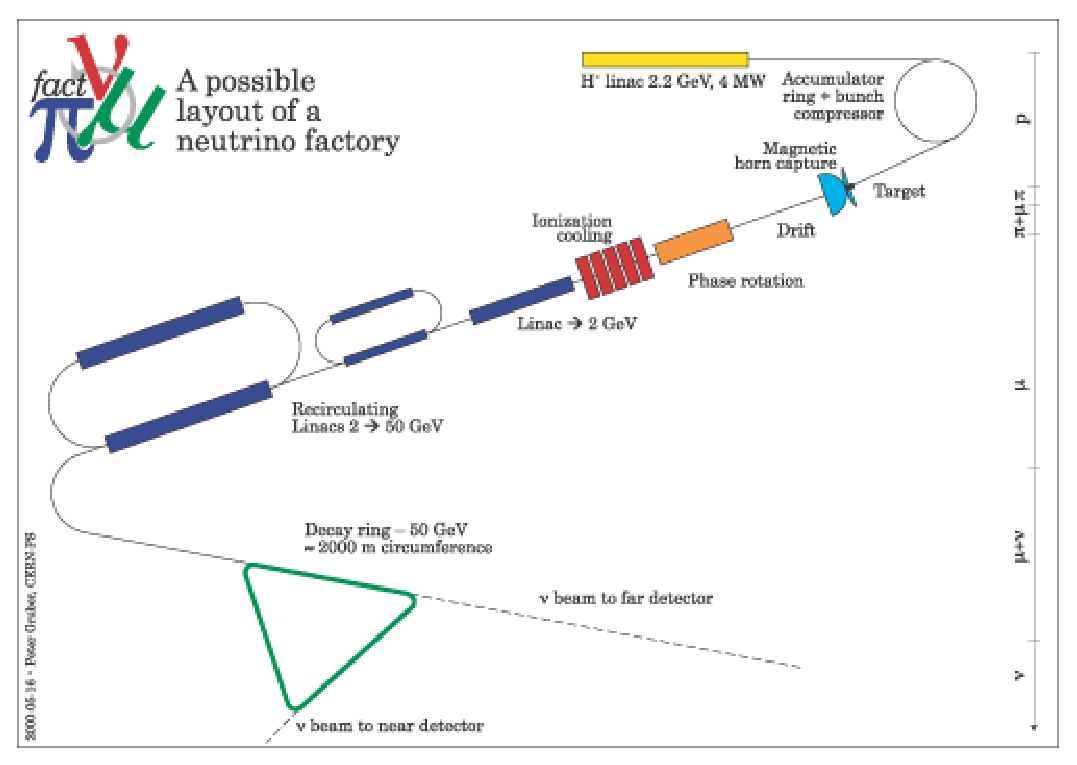
\includegraphics[bbllx=14,bblly=14,bburx=515,bbury=365,width=11cm,height=6cm]{./figs_FFAG_introSlides/CERN_nf_triangle.eps} \\

\vspace{-55mm}
{\footnotesize \hspace{0cm}  ~ ~ ~ ~ $A_n=1.5\pi$cm/$\pm20\%$}

\vspace{25mm}

{\footnotesize \hspace{0cm} $A_n=3\pi$cm/$\pm2\%$}
\vspace{10mm}

\rule{20mm}{.4mm}\\
\LARGE US NuFact 
\vspace{-25mm} 

\hspace{35mm}\includegraphics*[bbllx=160,bblly=30,bburx=235,bbury=280,width=2cm,angle=-90]{./figs_FFAG_introSlides/study-2.eps}   \\

\vspace{-10mm}
\hspace{-7mm}\includegraphics*[bbllx=0,bblly=0,bburx=263,bbury=384,width=8cm,angle=-90]{./figs_FFAG_introSlides/tabCost.eps}

~~~~~~~~~~~~~~

\end{minipage}\hspace{5mm}
\begin{minipage}[b]{.55\linewidth}

\large
The Europe and the two US NuFact studies propose  to  accelerate muons up to the storage energy (20 or 50~GeV) 
by means of  one or two 4- or 5-pass RLA's. RLA's are complicated machines (spreaders, combiners), hence expensive. 


\medskip

\LARGE The Japan NuFact

\large

J-Parc: 50-GeV, $3.3\, 10^{14}$~ppp at 0.3 Hz (15~$\mu$A) ~/~ 0.75~MW

Four muon FFAG's~:  0.2-1~GeV, 1-3,  3-10 (SC),  10-20~(SC). 

No cooling,  compact (R$\approx$200m)

\medskip

{\normalsize 30ns/300$\pm$50\%~MeV bunch } %~/~  $\approx$5~eV.s acceptance}

\vspace{-20mm}

\hspace{-1cm}\includegraphics[angle=-90,width=8cm]{./figs_FFAG_introSlides/g3D-gnuplot.eps}

\vspace{-6cm}
%%BoundingBox: 0 0 612 792
\includegraphics*[bbllx=100,bblly=470,bburx=660,bbury=792,width=19cm]{./figs_FFAG_introSlides/nuFactJ.eps2}

\normalsize 
Acceleration rate is lower than RLA, requires larger distance, but, 
acceptance is larger  both transversally (twice~: DA $3~\pi$cm norm. at $\delta p=0$) %NIMA 503 (2003) Keil 
and longitudinally ($\approx5$~eV.s). 
Hence achieve comparable production rate~:   $\approx 10^{20}$ muon decays per year (1~MW p power). 
\end{minipage}\hspace{0mm}




%\clearpage


\large     

\begin{minipage}{.33\linewidth}

~~~~~~~~

\vspace{10mm} 

\hspace{-10mm} \includegraphics*[bbllx=0,bblly=0,bburx=1024,bbury=768,width=9.7cm]{./figs_FFAG_introSlides/PoPFFAG.eps}

\vspace{-90mm} 
\hspace{-10mm}\includegraphics[width=6.cm]{./figs_FFAG_introSlides/popMagnet.eps}

\vspace{55mm}

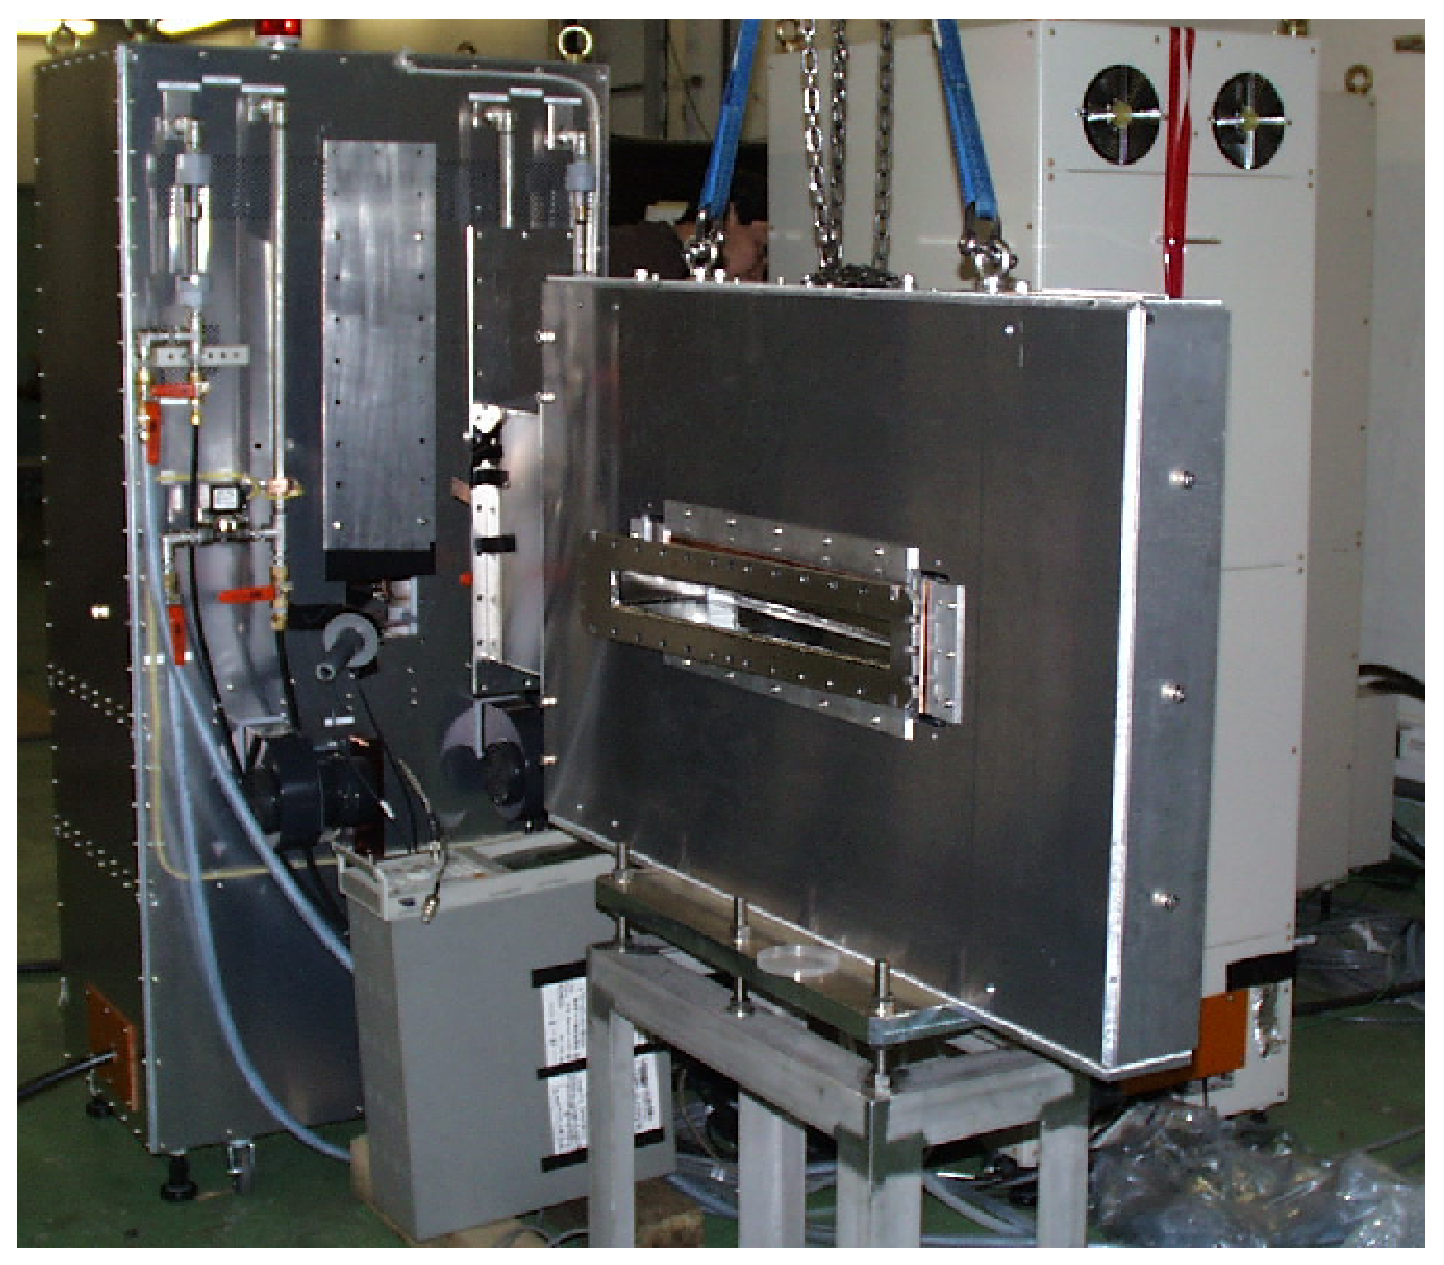
\includegraphics[width=5.cm]{./figs_FFAG_introSlides/FFAG31_cavity_Part.eps}

\vspace{-3mm}

\hspace{5mm} \includegraphics*[bbllx=340,bblly=540,bburx=650,bbury=740,width=10.5cm]{./figs_FFAG_introSlides/dNudB.eps}

~~~~~~~~

~~~~~~~~~

~~~~~~~~~

~~~~~~~~~

\end{minipage}\hspace{0mm}
\begin{minipage}{.65\linewidth}
\section{\LARGE  KEK proton  prototypes}

\subsection*{\Large     $\bullet$ POP - Proof of principle, the first proton FFAG}
\begin{center}  First beam Dec. 1999. \end{center}
\large   
  \begin{center}
                   {\bf \Large   \underline{[Typical] data}} 
   \begin{tabular}{llccc}
\\[-3mm]
      &$E_{inj} - E_{max}$  &    keV  &     50 - 500     &             \\
      &orbit radius& m   &    0.8 - 1.14    &          \\
\multicolumn{2}{l}{\it \underline{Optics}}   \\
      & lattice    &     &  DFD    & \\
      & number of cells& &     8            &            \\
      &   K        &     &      2.5         &    ($B=B_0 (r/r_0)^K \, \mathcal{F}(\theta)$) \\
      &$\beta_r,~\beta_z$ max.&m  &   0.7  &        \\
      &$\nu_r~/~\nu_z$&  &    2.2~/~1.25  &   \it tunable via $B_F/B_D$ ratio        \\
%      & radial accept. & $\pi$cm &   0.4    &  \raisebox{1ex}[0mm][0mm]{\it mechanical limit is}  \\
%      &            &     &                  &  \raisebox{2ex}[0mm][0mm]{\it injection inflector}   \\[-2ex]
%      & vertical accept. & $\pi$cm &   \\
\multicolumn{2}{l}{\it  \underline{Magnet}}&\multicolumn{2}{l}{ \fbox{ \bf high field,  non-linear gradient}}& \it sector triplet \\
&$\theta_D~/~\theta_F$, core&deg&   2.8~/~14      &          \\ 
      & $B_D~/~B_F$& T   &    0.04-0.13~/~0.14-0.32    &   \it  $r_{inj} \rightarrow r_{max}$       \\
      &   gap      & cm  &    30-9        &   \it        $gap = g_0 (r_0/r)^K$                  \\[1ex]
\multicolumn{2}{l}{\it \underline{Injection}}& &multi- or single-turn & \bigg\{ \raisebox{1ex}[0mm][0mm]{\it electrostatic inflector} \\
      &        &         &                  &                \raisebox{2ex}[0mm][0mm]{\it  + 2 bumpers}  \\[-2ex]
\multicolumn{2}{l}{\it \underline{Extraction}}& \multicolumn{3}{l}{\fbox{ \bf massless septum } exprmnt} \\
\multicolumn{2}{l}{\it  \underline{Acceleration}}  \\
& \multicolumn{2}{l}{\it  Amorphous MA cavity} & \multicolumn{2}{l}{\fbox{ \bf broad band, high $\vec E$ RF} ; \fbox{ \bf 2-beam accel.} } \\
      & swing      & MHz &   0.6 - 1.4      &  \\
      &harmonic    &     &          1       &  \\
      &voltage p-to-p& kV&   1.3 - 3        &  \\
      & cycle time & ms  &      1       &      \fbox{  \it fast acceleration } \\
      & rep. rate  & kHz &      1         &     \fbox{  \it high average current } \\
      &     $\dot B$ &T/s&    180        &       \\
   \end{tabular}
  \end{center}

~~~~~~~~~

~~~~~~~~~

~~~~~~~~~

~~~~~~~~~

~~~~~~~~~

\end{minipage}



\clearpage


\large   

\begin{minipage}[b]{.36\linewidth}
\hspace{-10mm} \includegraphics*[bbllx=14,bblly=14,bburx=1701,bbury=1155,width=10.cm]{./figs_FFAG_introSlides/118-1825_IMG.eps}

``return yoke free'' magnet % (+shunt yokes)

\includegraphics*[width=7.cm]{./figs_FFAG_introSlides/FigTriplet.eps}

\hspace{-0mm}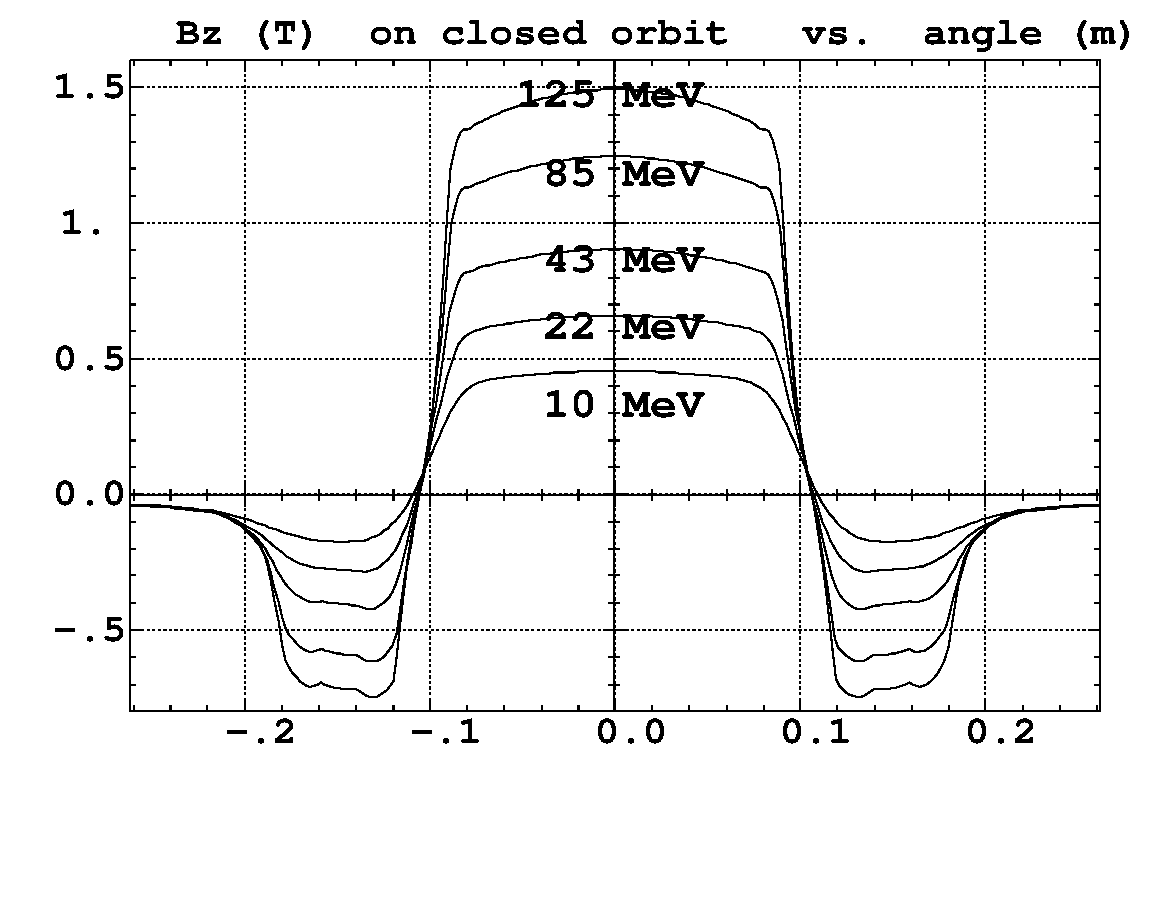
\includegraphics[bbllx=20,bblly=120,bburx=567,bbury=480,width=9.00cm,height=4cm]{./figs_FFAG_introSlides/fieldOnCO.eps}

\mbox{ \hspace{-10mm}
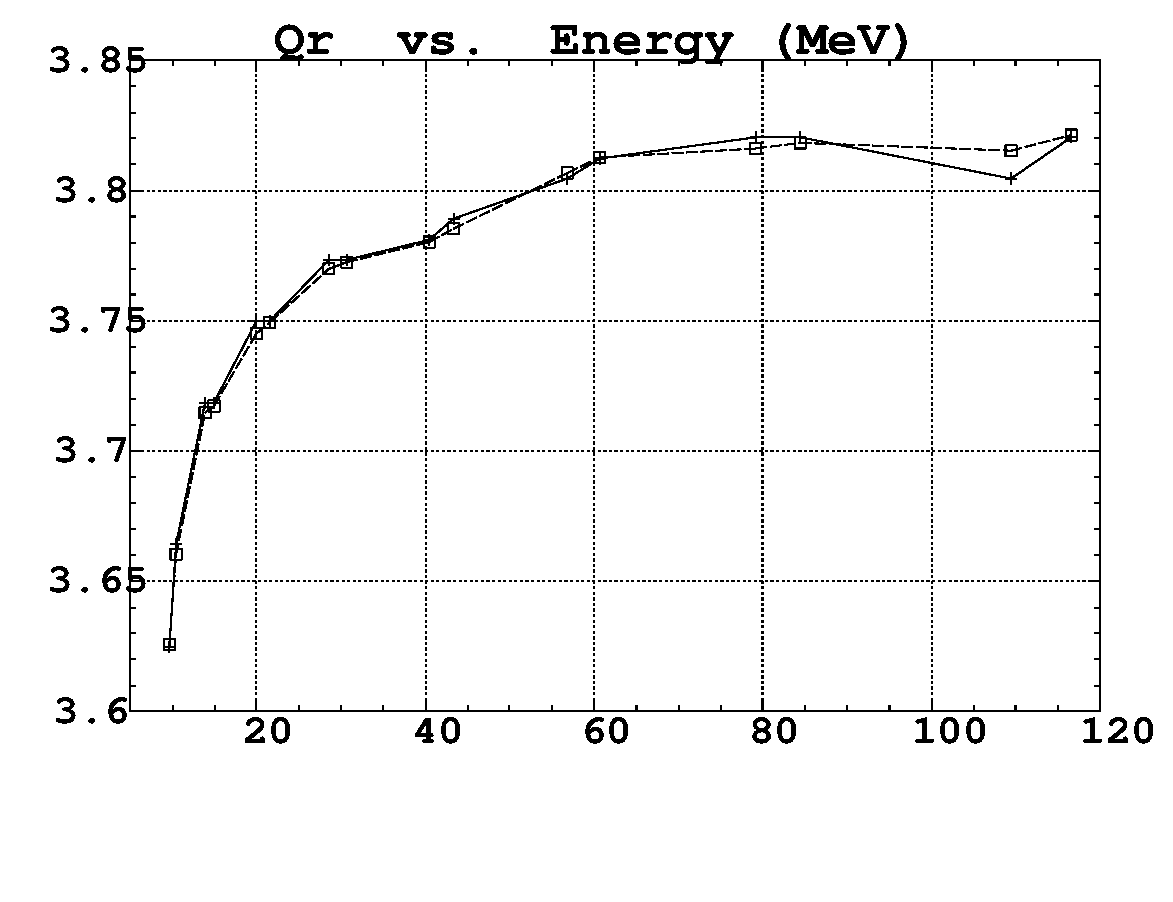
\includegraphics[bbllx=20,bblly=120,bburx=567,bbury=500,width=5.400cm]{./figs_FFAG_introSlides/QrVsE.eps}
\hspace{-2mm}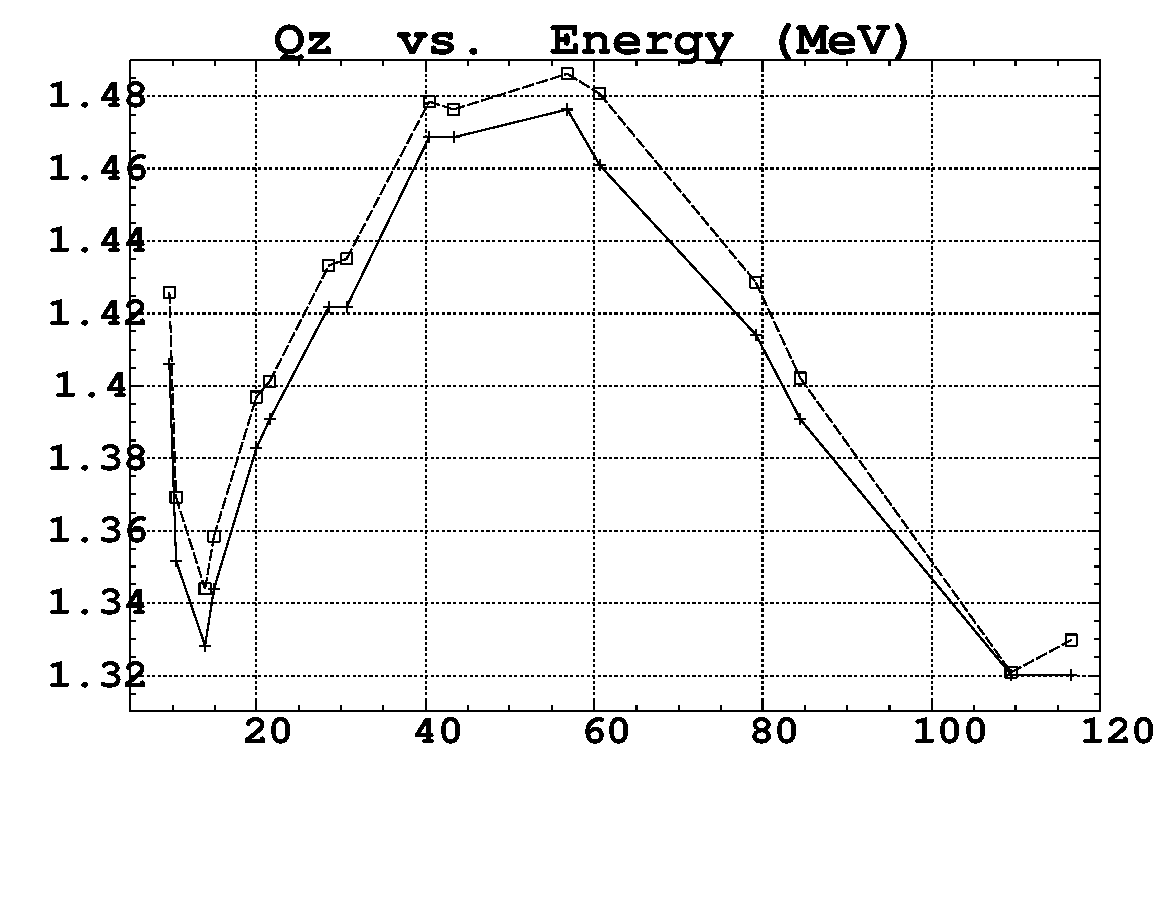
\includegraphics[bbllx=20,bblly=120,bburx=567,bbury=500,width=5.400cm]{./figs_FFAG_introSlides/QzVsE.eps}
}

~~~~~~~~~~~~~

\end{minipage}\hspace{0mm}
\begin{minipage}[b]{.65\linewidth}
\subsection*{\Large      $\bullet$ The 150~MeV machine}
\begin{center}  First operation 2003. \end{center}
\large   
  \begin{center}
                   {\bf \LARGE   \underline{[Typical] data}} 
   \begin{tabular}{llccc}
\\[-3mm]
      &$E_{inj} - E_{max}$  &    MeV  &     12 - 150     &             \\
      &orbit radius& m   &    4.47 - 5.20  &          \\
\multicolumn{2}{l}{\it \underline{Optics}}   \\
      & lattice    &     &   DFD     & \it 9.5~deg. drift   \\
      & numb. of cells& &      12          &            \\
      &   K        &     &      7.6         &     ($B=B_0 (r/r_0)^K \, \mathcal{F}(\theta)$) \\
      &$\beta_r~/~\beta_z$ max.&m  &    2.5~/~4.5  &        \\
      &$\nu_r~/~\nu_z$&  &    3.7~/~1.3  &     \it tunable via $B_F/B_D$ ratio   \\
      & $\alpha, ~ \gamma_{tr}$ &&       0.13, ~~ 2.95          & \it $1/(1+K)$, ~~ $(1+K)^{1/2}$    \\
      &  $\mathcal{R}/\rho|_{E_{max}}$ &&          5.4             \\
\multicolumn{2}{l}{\it  \underline{Magnet}}  & \multicolumn{3}{l}{\fbox{ \bf Return yoke free magnet} } \\
&$\theta_D~/~\theta_F$   &deg&   3.43~/~10.24    &          \\ 
      & $B_D~/~B_F$& T   &     0.2-0.78~/~0.5-1.63    &   \it $r_{inj} \rightarrow r_{max}$                \\
      &   gap      & cm  &    23.2 - 4.2        &   \it at $r_{inj}$ - $r_{max}$ ($gap = g_0 \left( \frac{r_0}{r}\right)^K$)      \\[1ex]
\multicolumn{2}{l}{\it \underline{Injection}}& &  multi-turn &\bigg\{  \raisebox{1ex}[0mm][0mm]{\it B-septum + E-septum}  \\
      &        &         &                  &                  \raisebox{2ex}[0mm][0mm]{\it  + 2 bumpers}  \\[-2ex]
\multicolumn{2}{l}{\it  \underline{Extraction}}& & single-turn & \fbox{\bf fast kicker (1kG, 150~ns)} \\
%     & extracted emittance&$\pi$mm.mrad&      50        &         \\
\multicolumn{2}{l}{\it  \underline{Acceleration}}&\multicolumn{3}{l}{\it  Amorphous MA, \fbox{ \bf broad band, high gradient RF} } \\
      & swing      & MHz &   1.5 - 4.5      &  \\
      &harmonic    &     &          1       &  \\
      &voltage p-to-p& kV&       2        &  \\
      &   $\phi_s$ & deg &       20         &         \\
      &   $\nu_s$  &     &    0.01 - 0.0026      &       \\
      &     $\dot B$ &T/s&     300     &       \fbox{  \it fast acceleration } \\
      &  rep. rate & Hz  &    250  &  \fbox{  \it high average current } \\
   \end{tabular}
  \end{center}

~~~~~~~~~~~~~~~~~~~~~~

\end{minipage}






\clearpage 

\Large 

\section{\LARGE KURRI KUCA }

\begin{minipage}{1\linewidth}

\black 

\vspace{-1ex}

An  ADS-R experiments, proton driver R/D

~ ~ ~ ~ -  First coupling to an ADS-R core, March 2009, 100 MeV beam

~ ~ ~ ~ -  Thorium-loaded ADS-R experiment, March 2010 : \blue  100 MeV, 30 Hz, 5 mW \black

\bigskip

\begin{minipage}{1\linewidth}

\mbox{
\begin{minipage}{.5\linewidth}


\centering
%\hspace{-10mm} 
\blue 

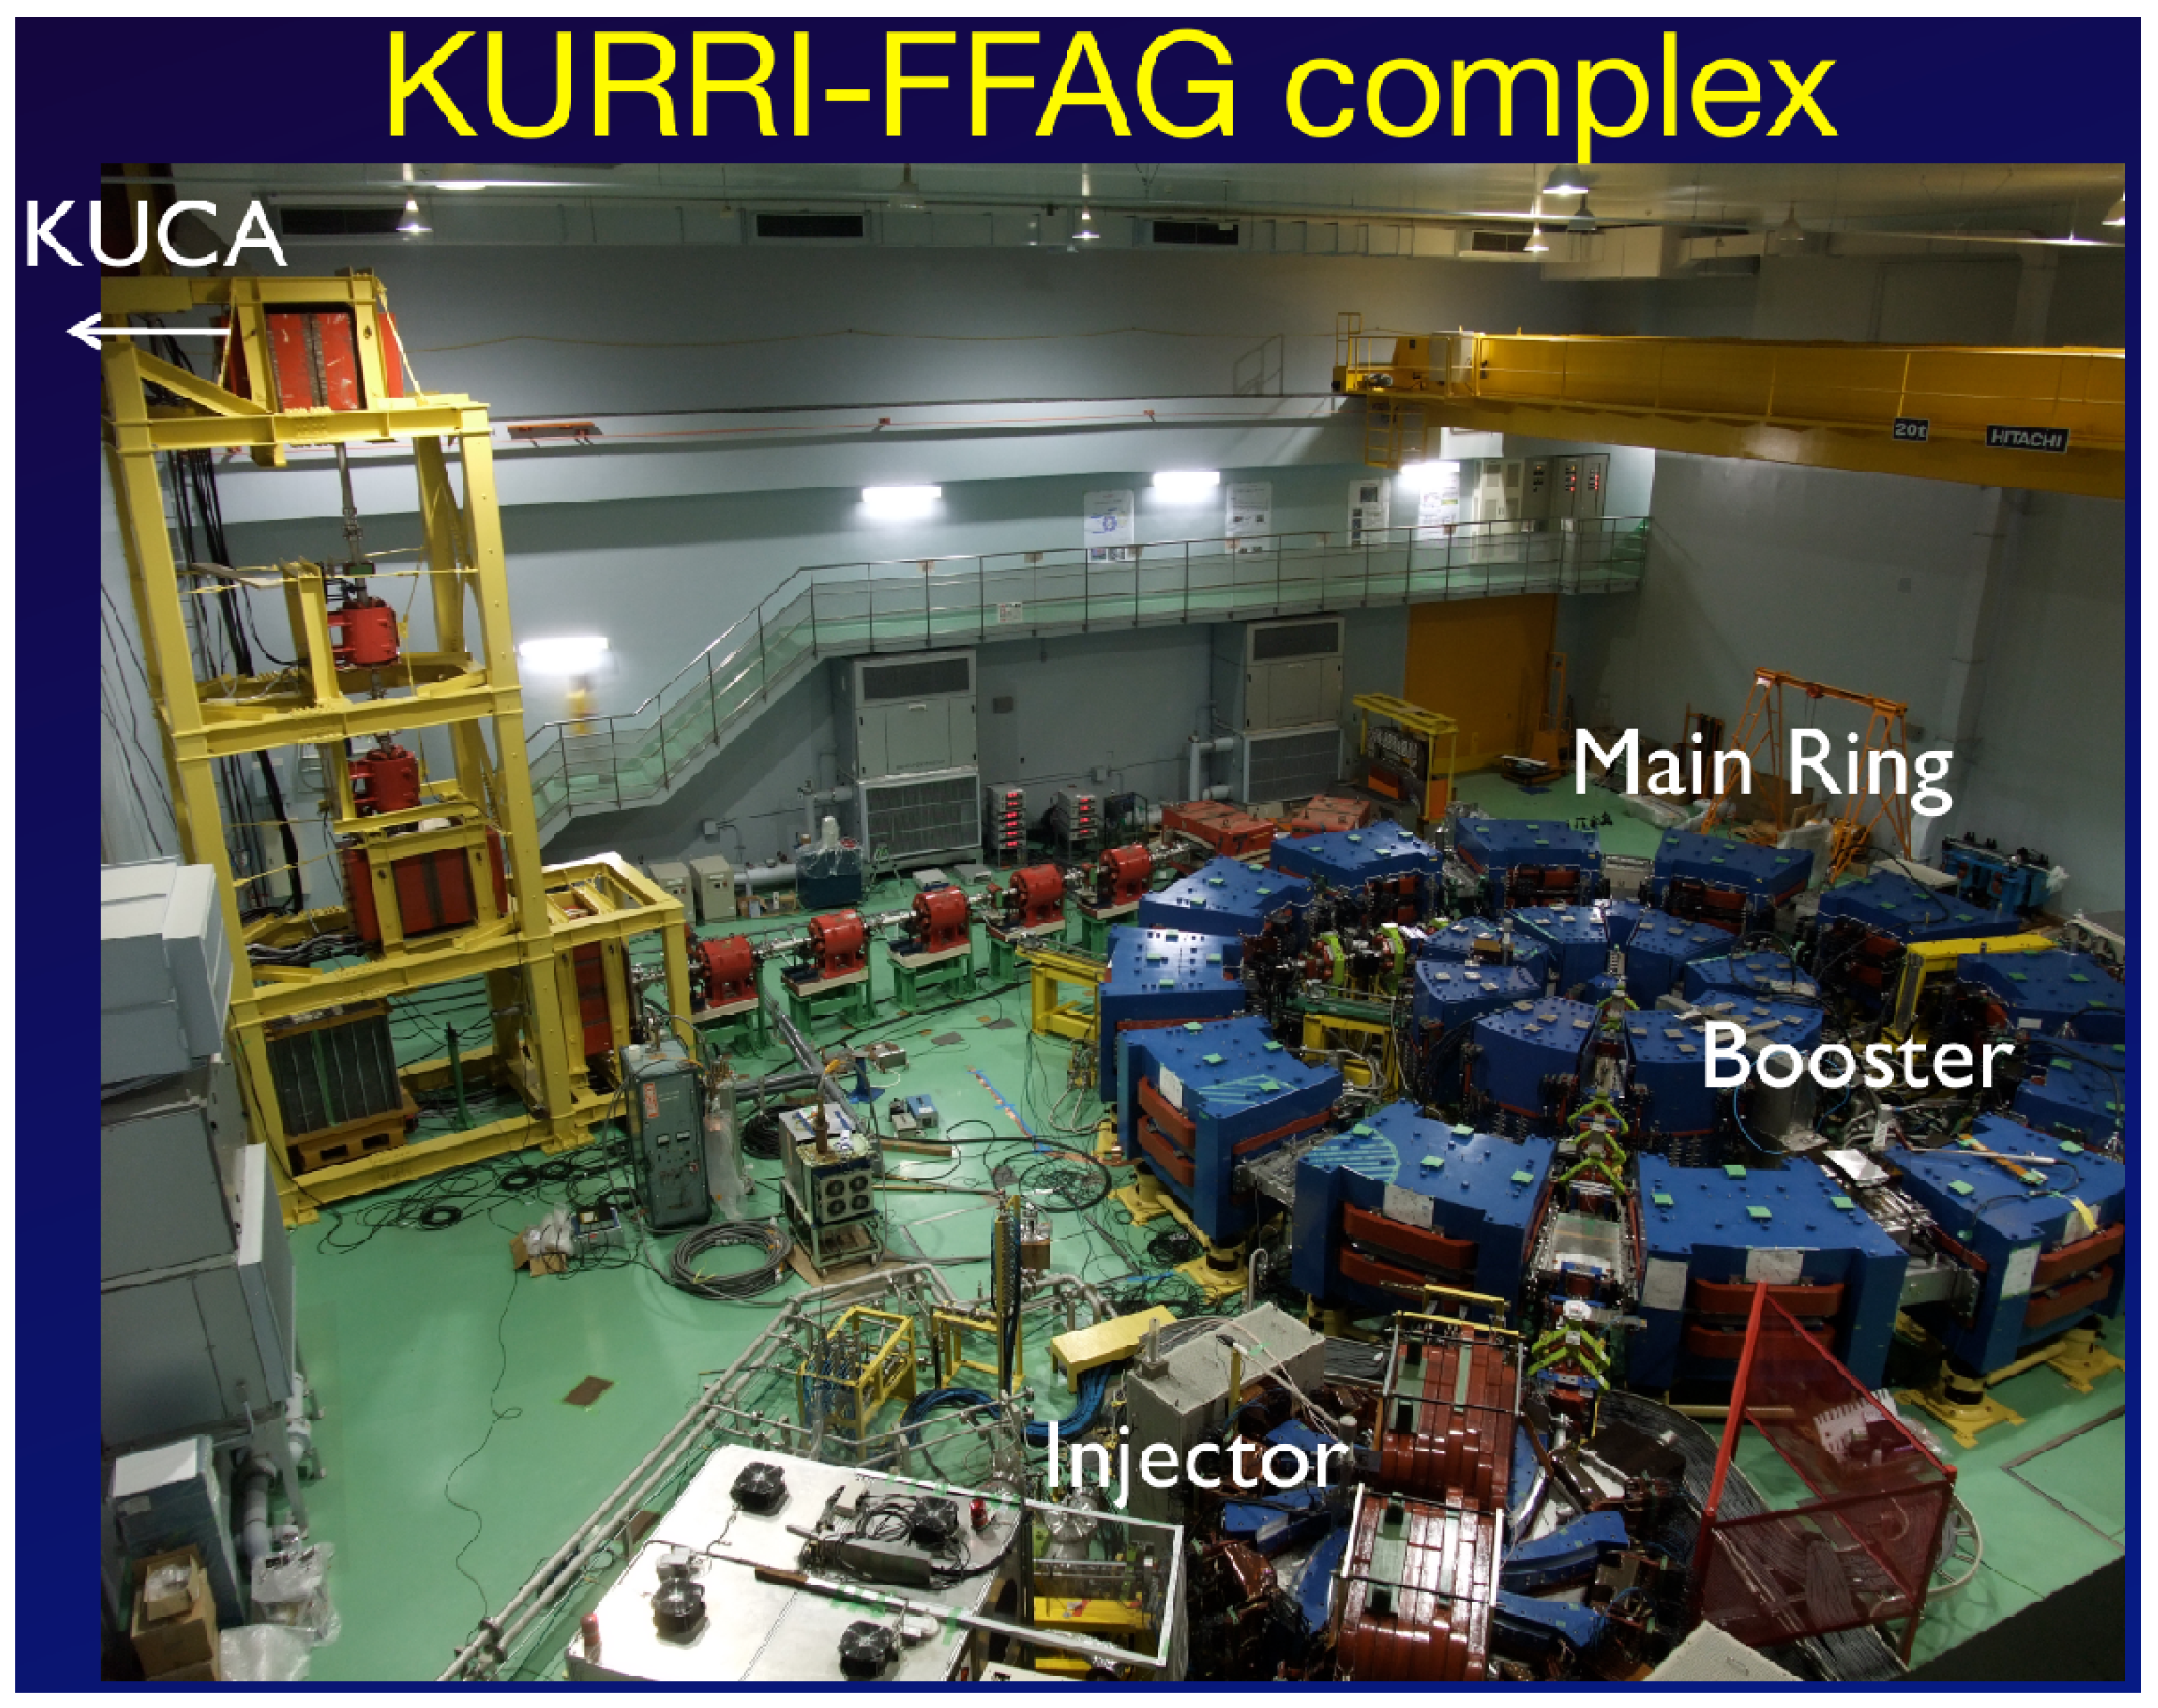
\includegraphics[width=0.7\linewidth]{./figs_FFAG_introSlides/kurriKucaAccel.eps}

\end{minipage}
\begin{minipage}{.49\linewidth}
\centering
%\hspace{-10mm} 

100-150 MeV proton, repetition rate 20-50 Hz \\[1ex]

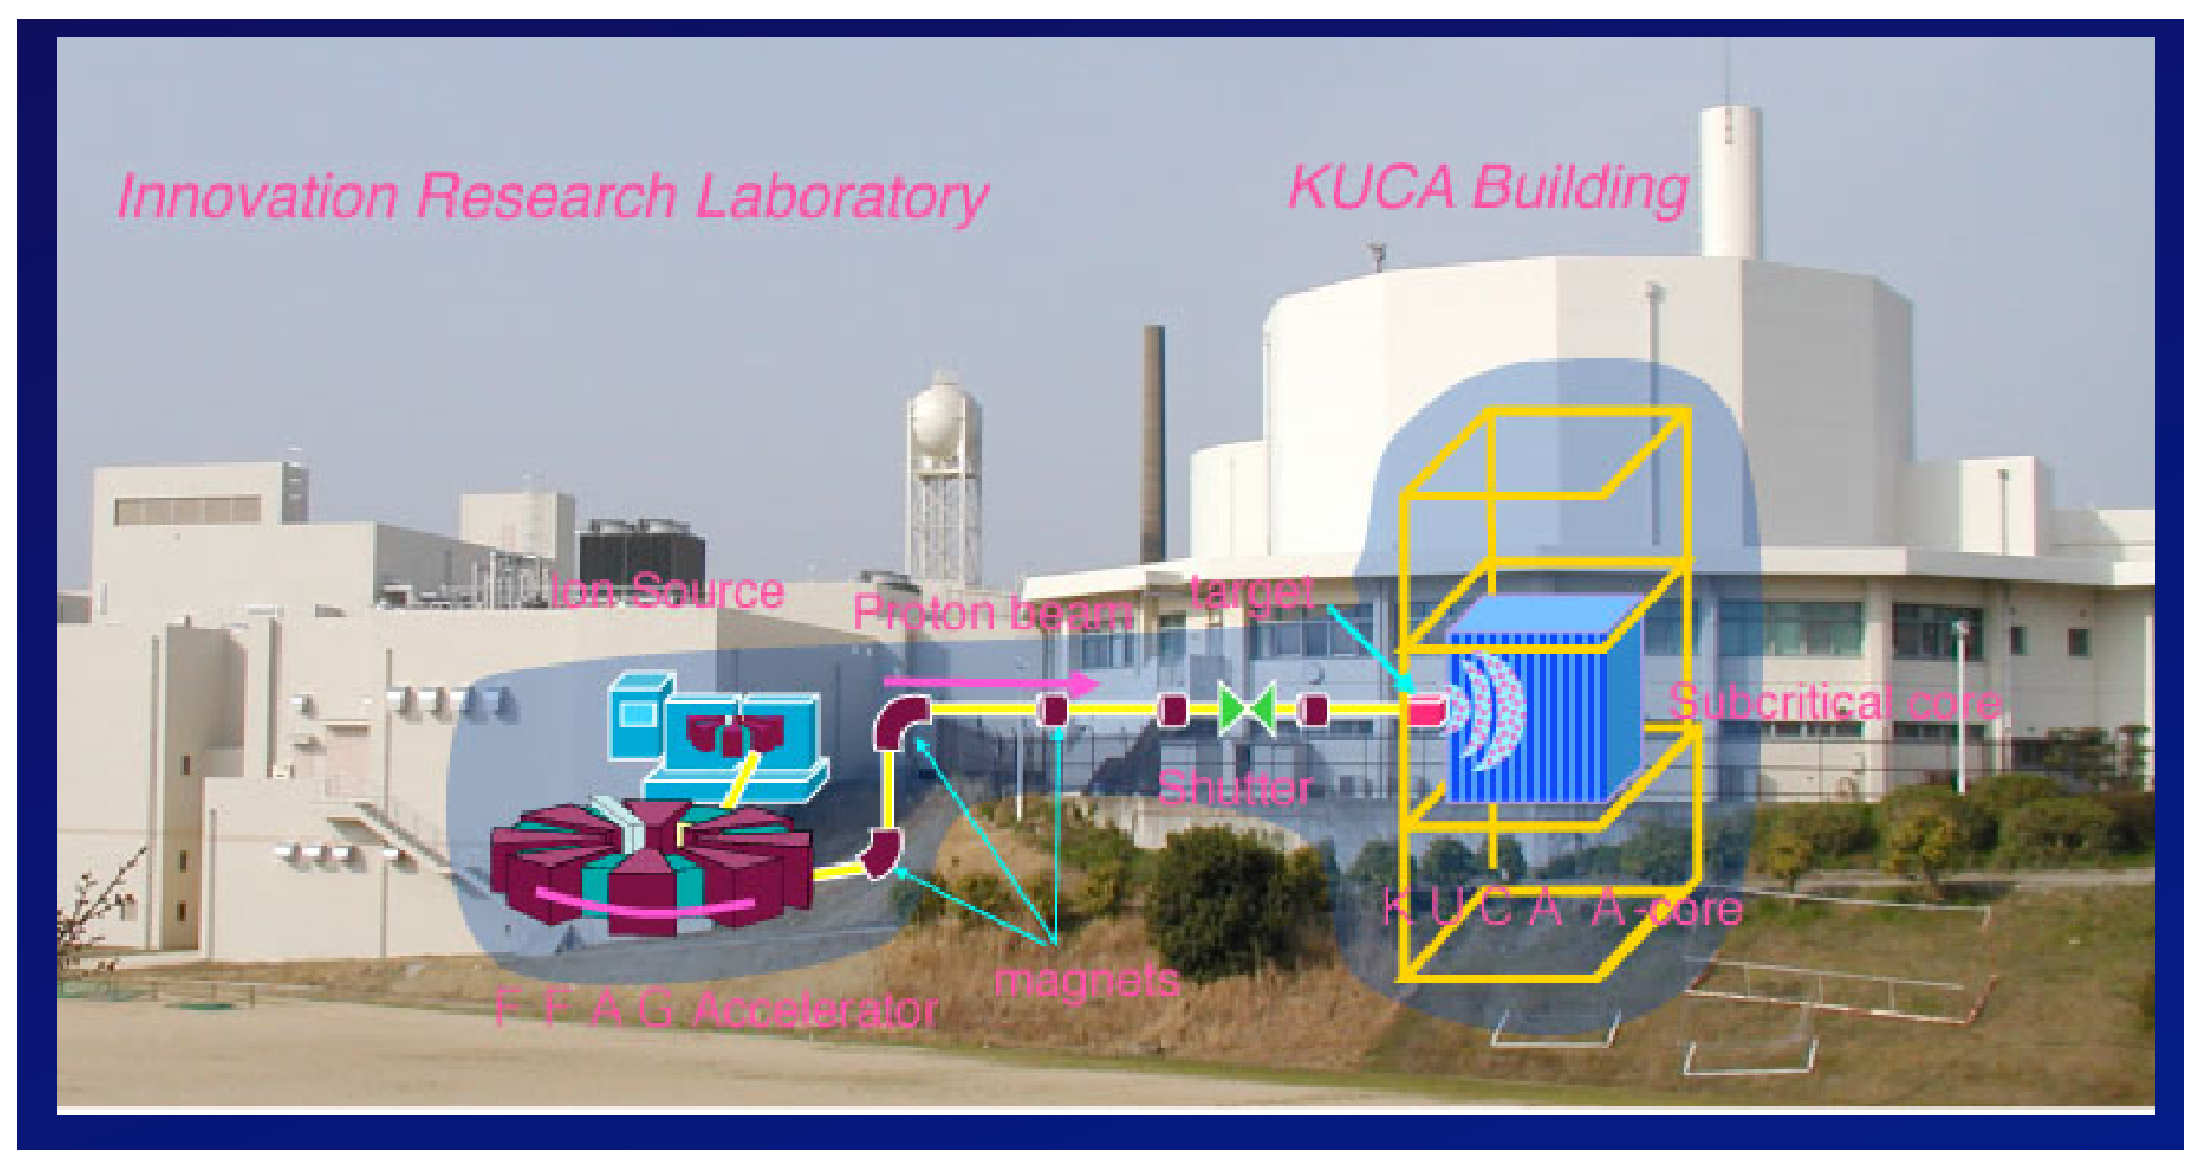
\includegraphics[height=0.5\linewidth]{./figs_FFAG_introSlides/kurriKuca.eps}

\vfill

\LARGE
\blue 

%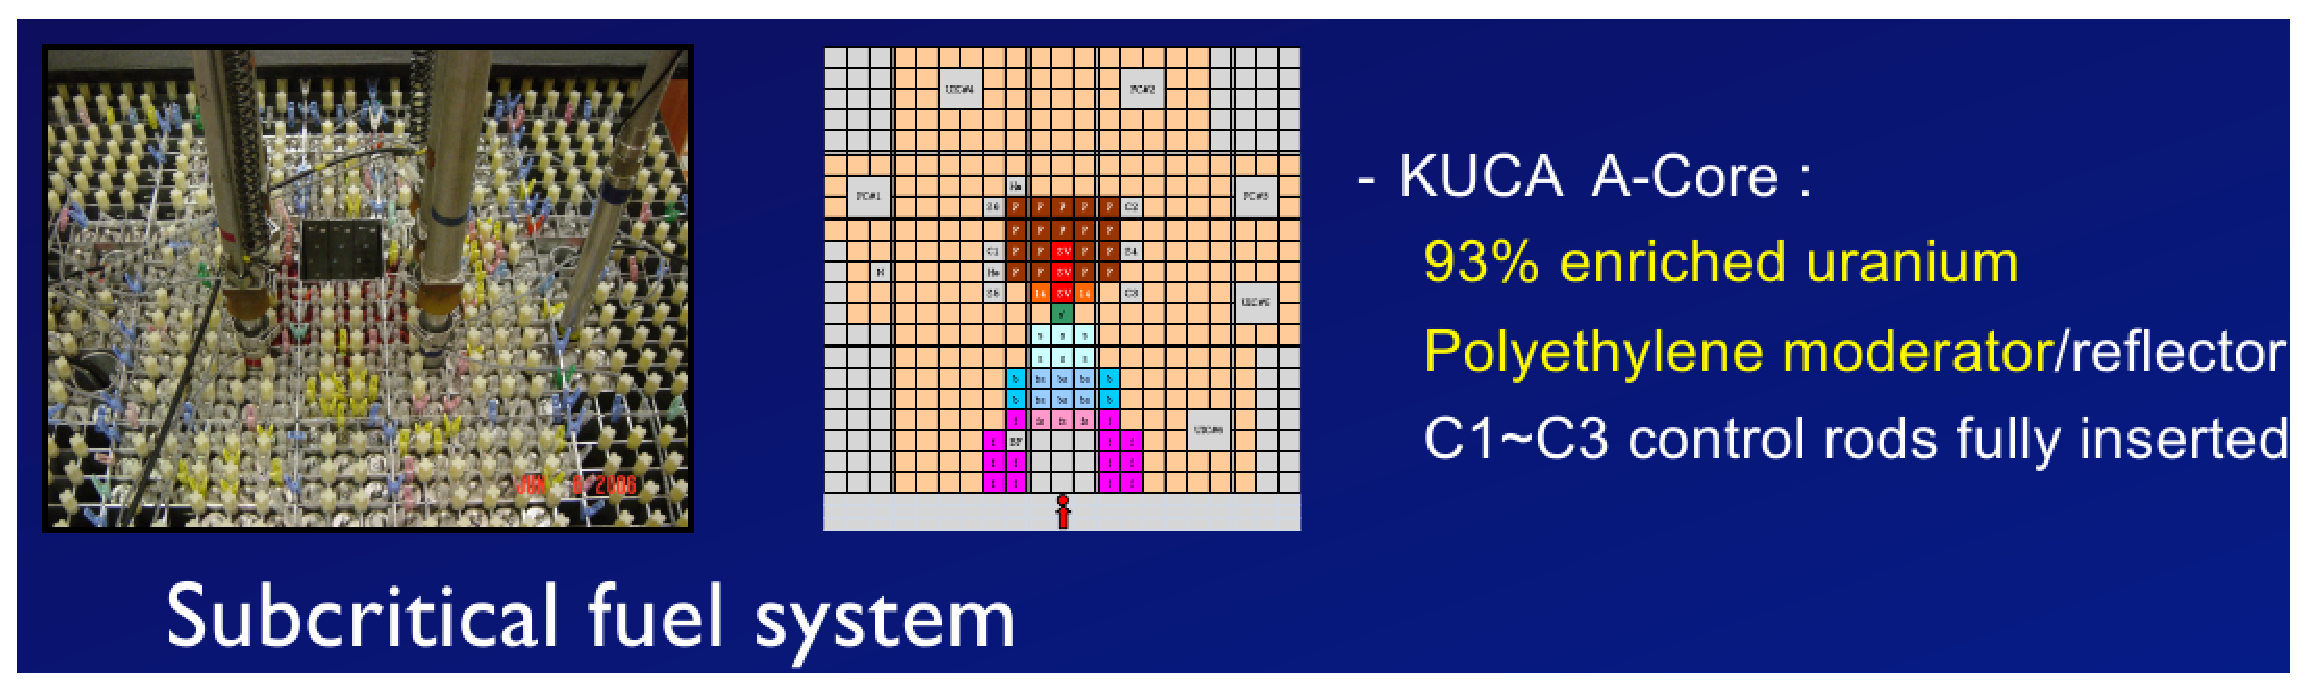
\includegraphics[height=5cm]{./figs_FFAG_introSlides/kurriFuelSystem.eps}

\end{minipage}
}


\begin{center}
\rule{80mm}{0.1mm}
\end{center}


\mbox{
\begin{minipage}{.49\linewidth}

{\blue \bf \nib \LARGE Upgrades : }

\medskip

\centering

\blue On-going :  H- charge exchange injection

Towards 10s of $\mu$Amp 

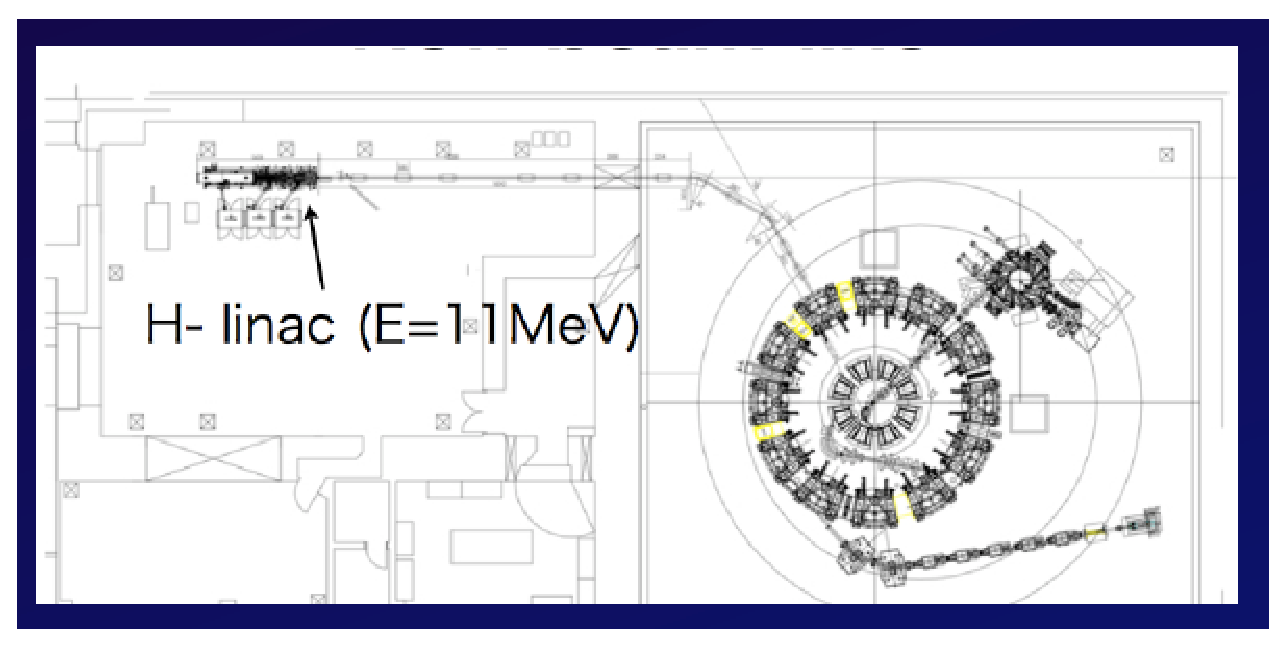
\includegraphics[width=1.\linewidth]{./figs_FFAG_introSlides/kurriH-Inj.eps}
%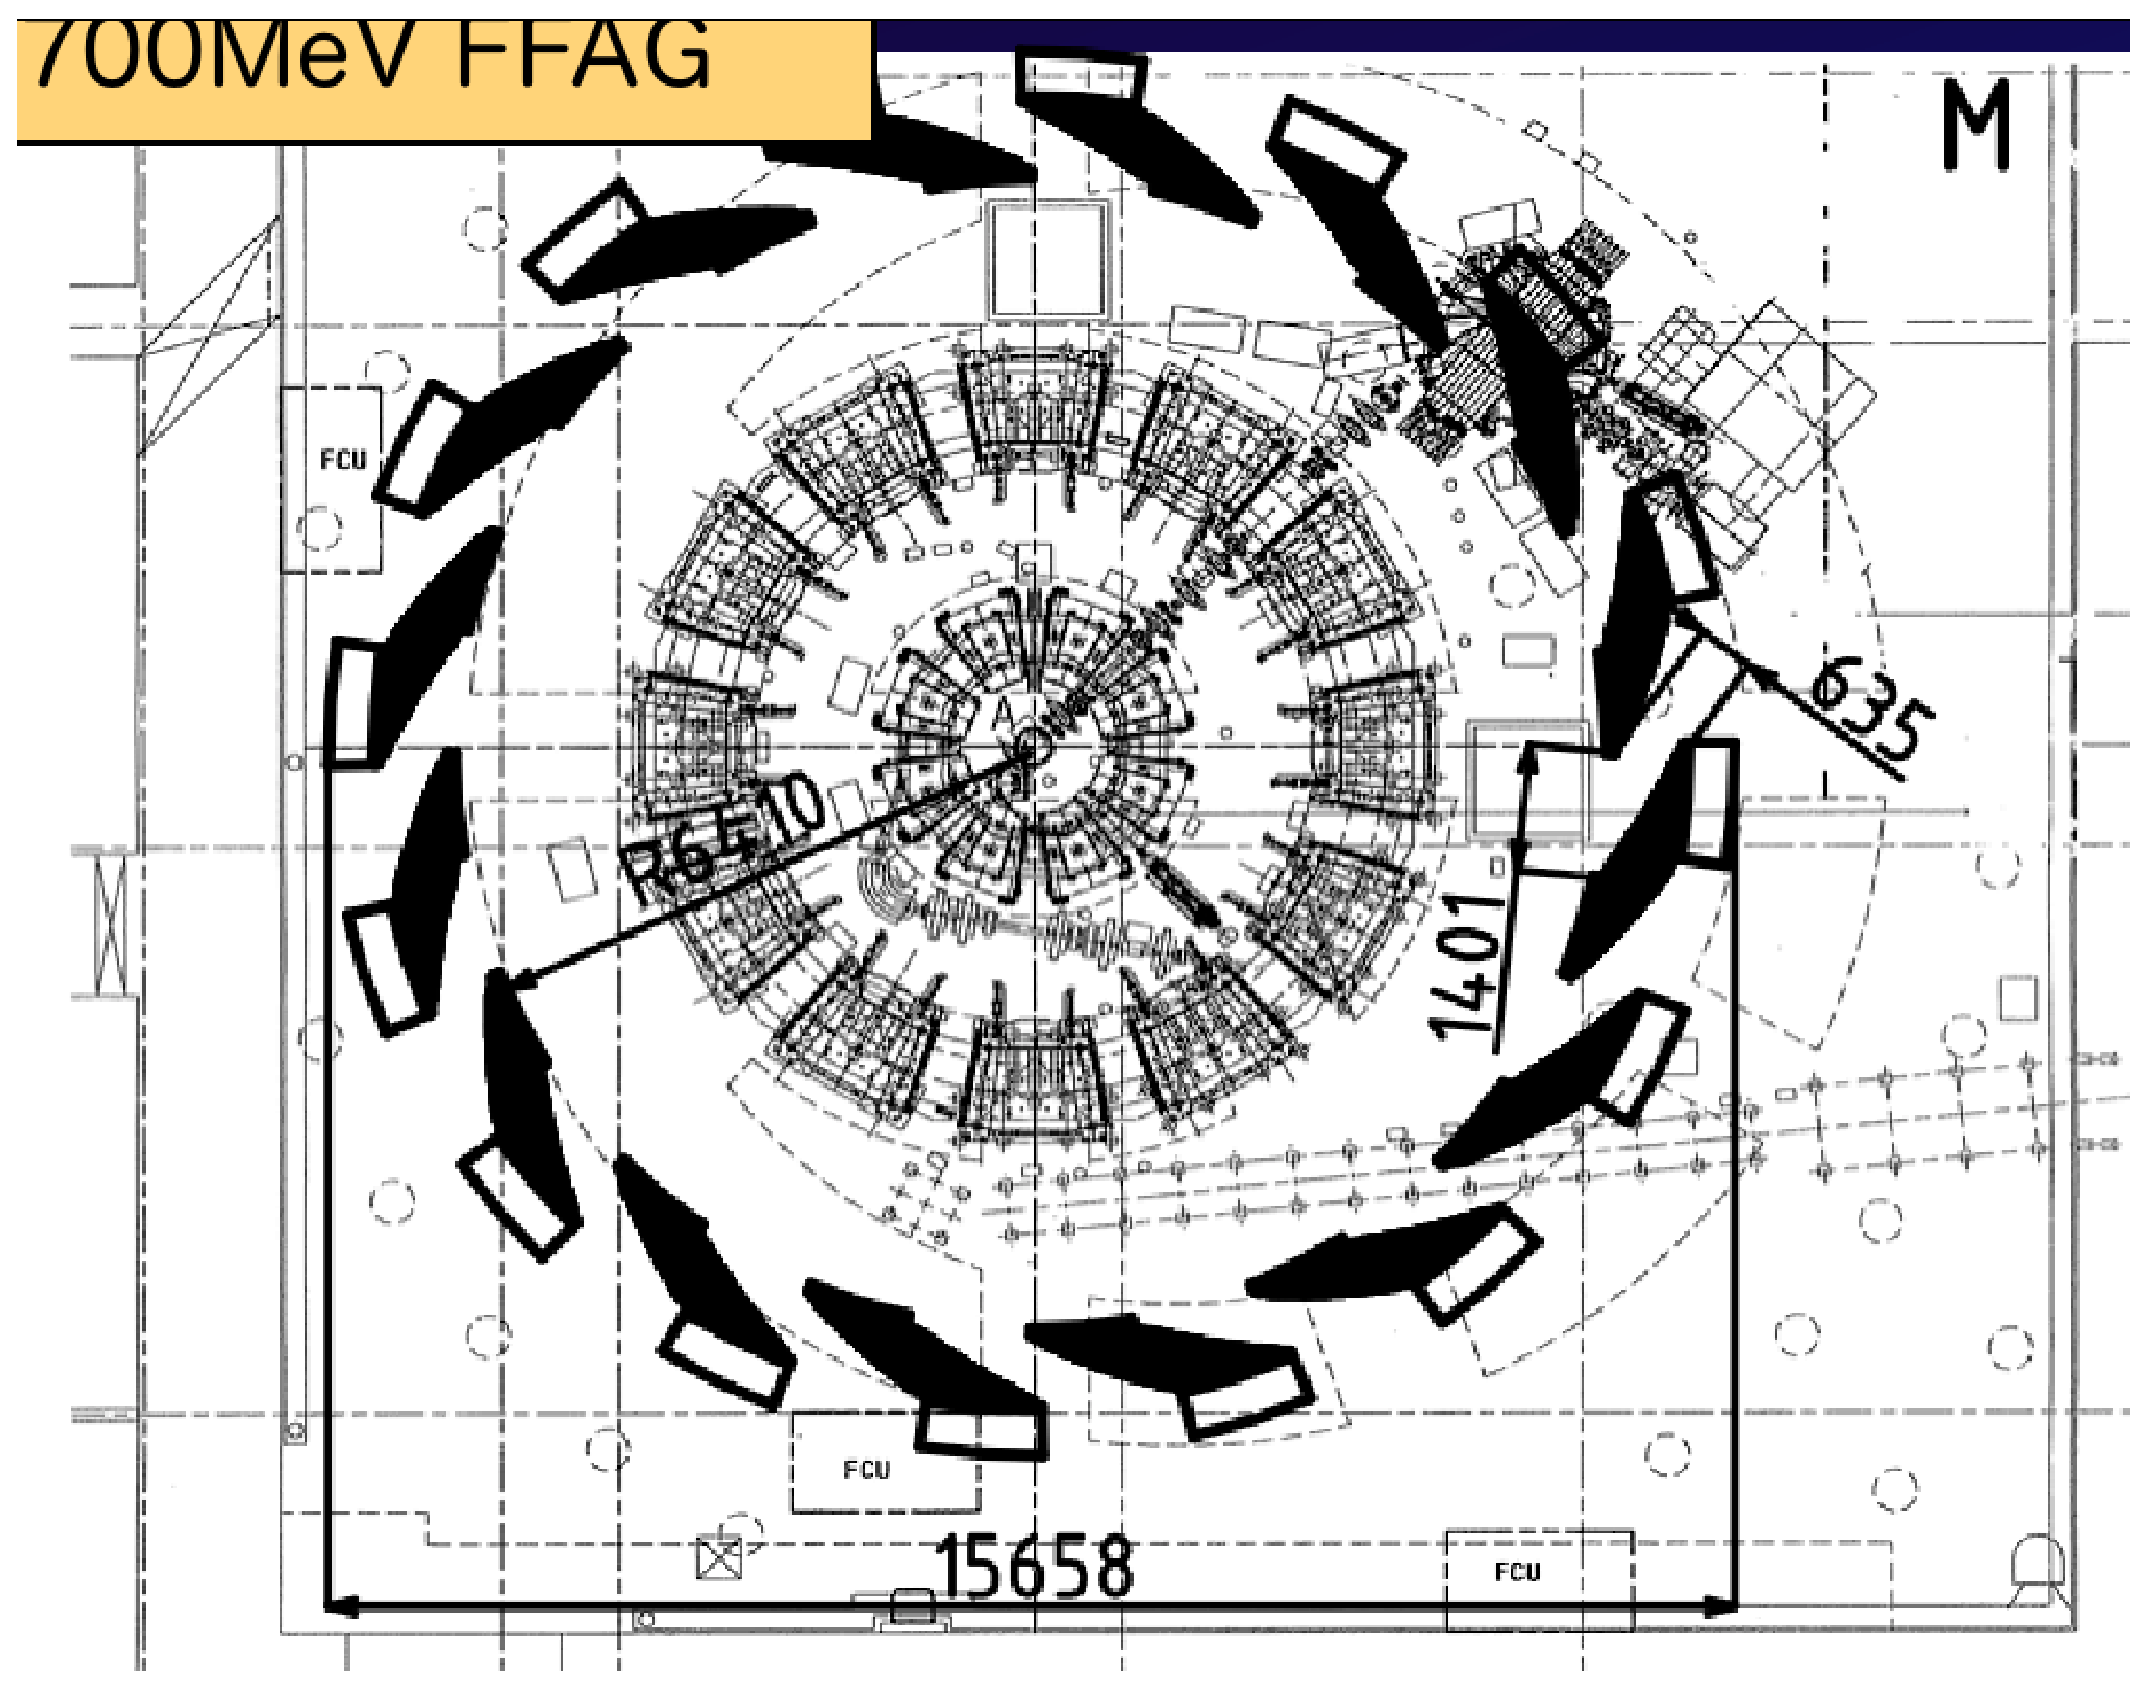
\includegraphics[height=11cm]{./figs_FFAG_introSlides/kurri700Accel.eps}

\end{minipage} ~ ~ 
\begin{minipage}{.55\linewidth}


\Large
\blue 

\medskip 


Planned~:  
 neutron flux increased by a factor 30.

Options~: additional 700~MeV spiral lattice FFAG,

 or 400~MeV quasi-isochronous FFAG

\centering 
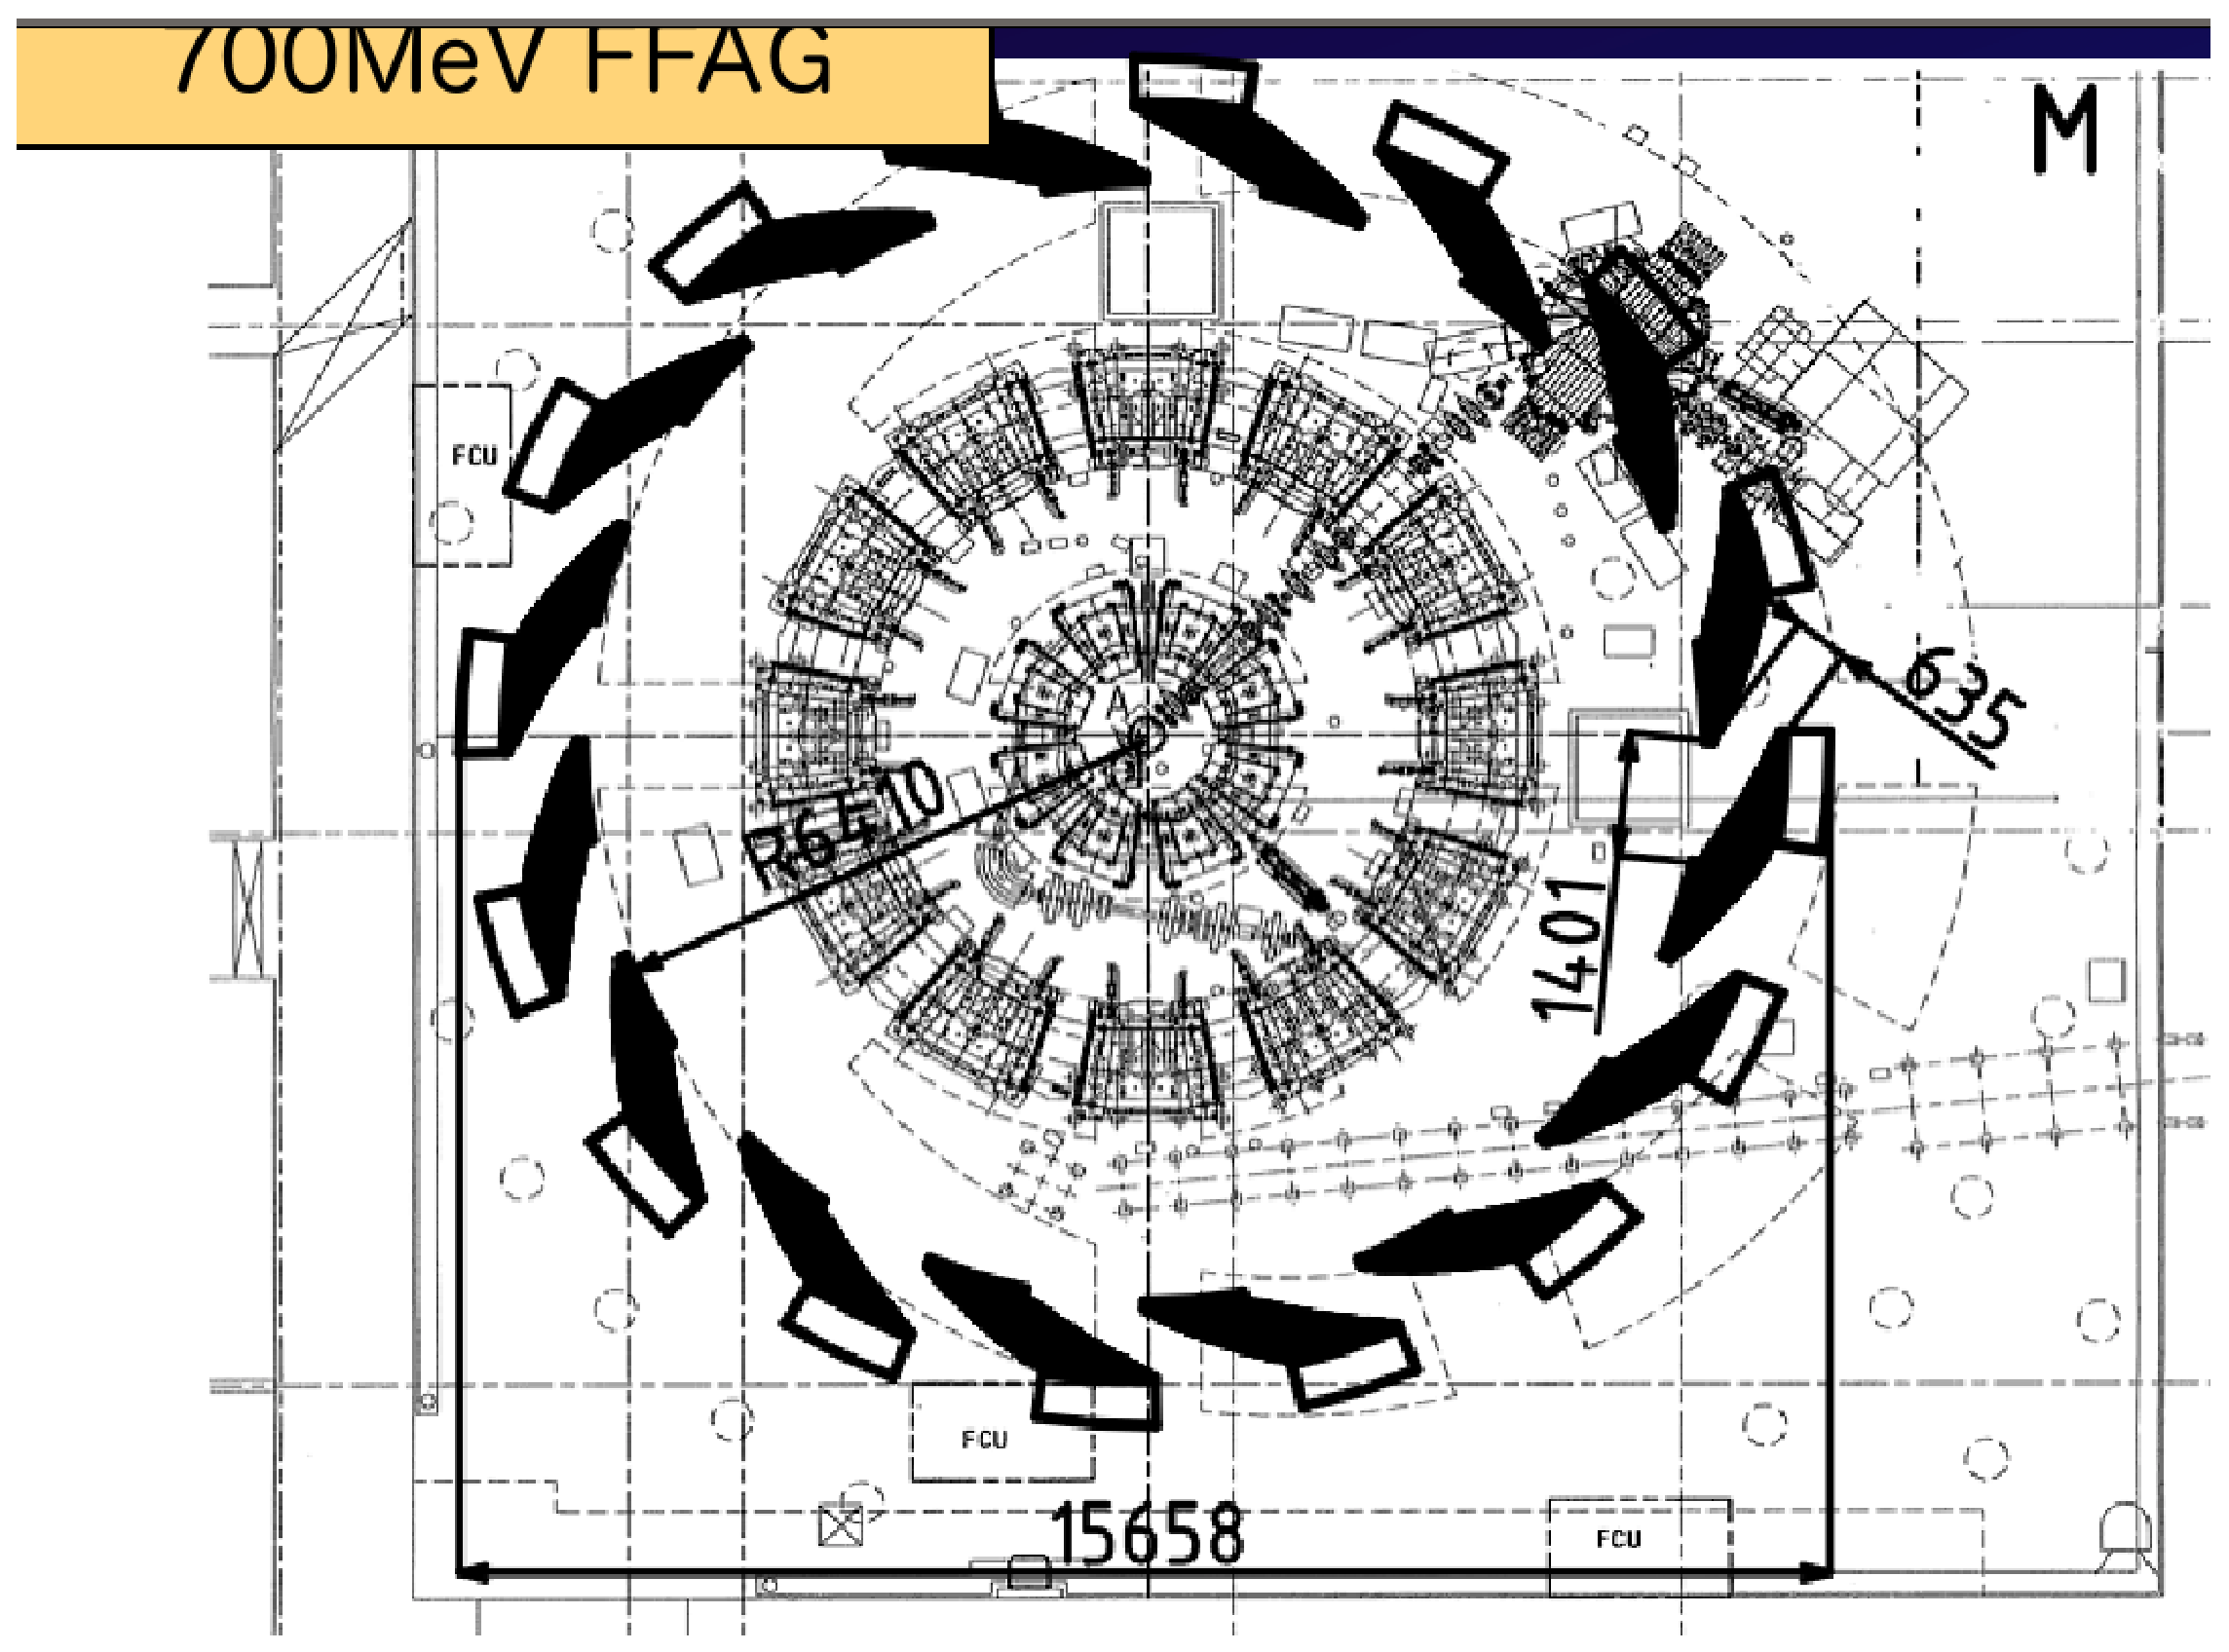
\includegraphics[width=.6\linewidth]{./figs_FFAG_introSlides/700MeVFFAG.eps}

\end{minipage} ~ ~ 
}

\end{minipage}
\end{minipage}



\clearpage

\begin{minipage}{1.\linewidth}

{\bf \LARGE KURRI KUCA 3-ring cascade}\\[10mm]
\begin{minipage}{.45\linewidth}


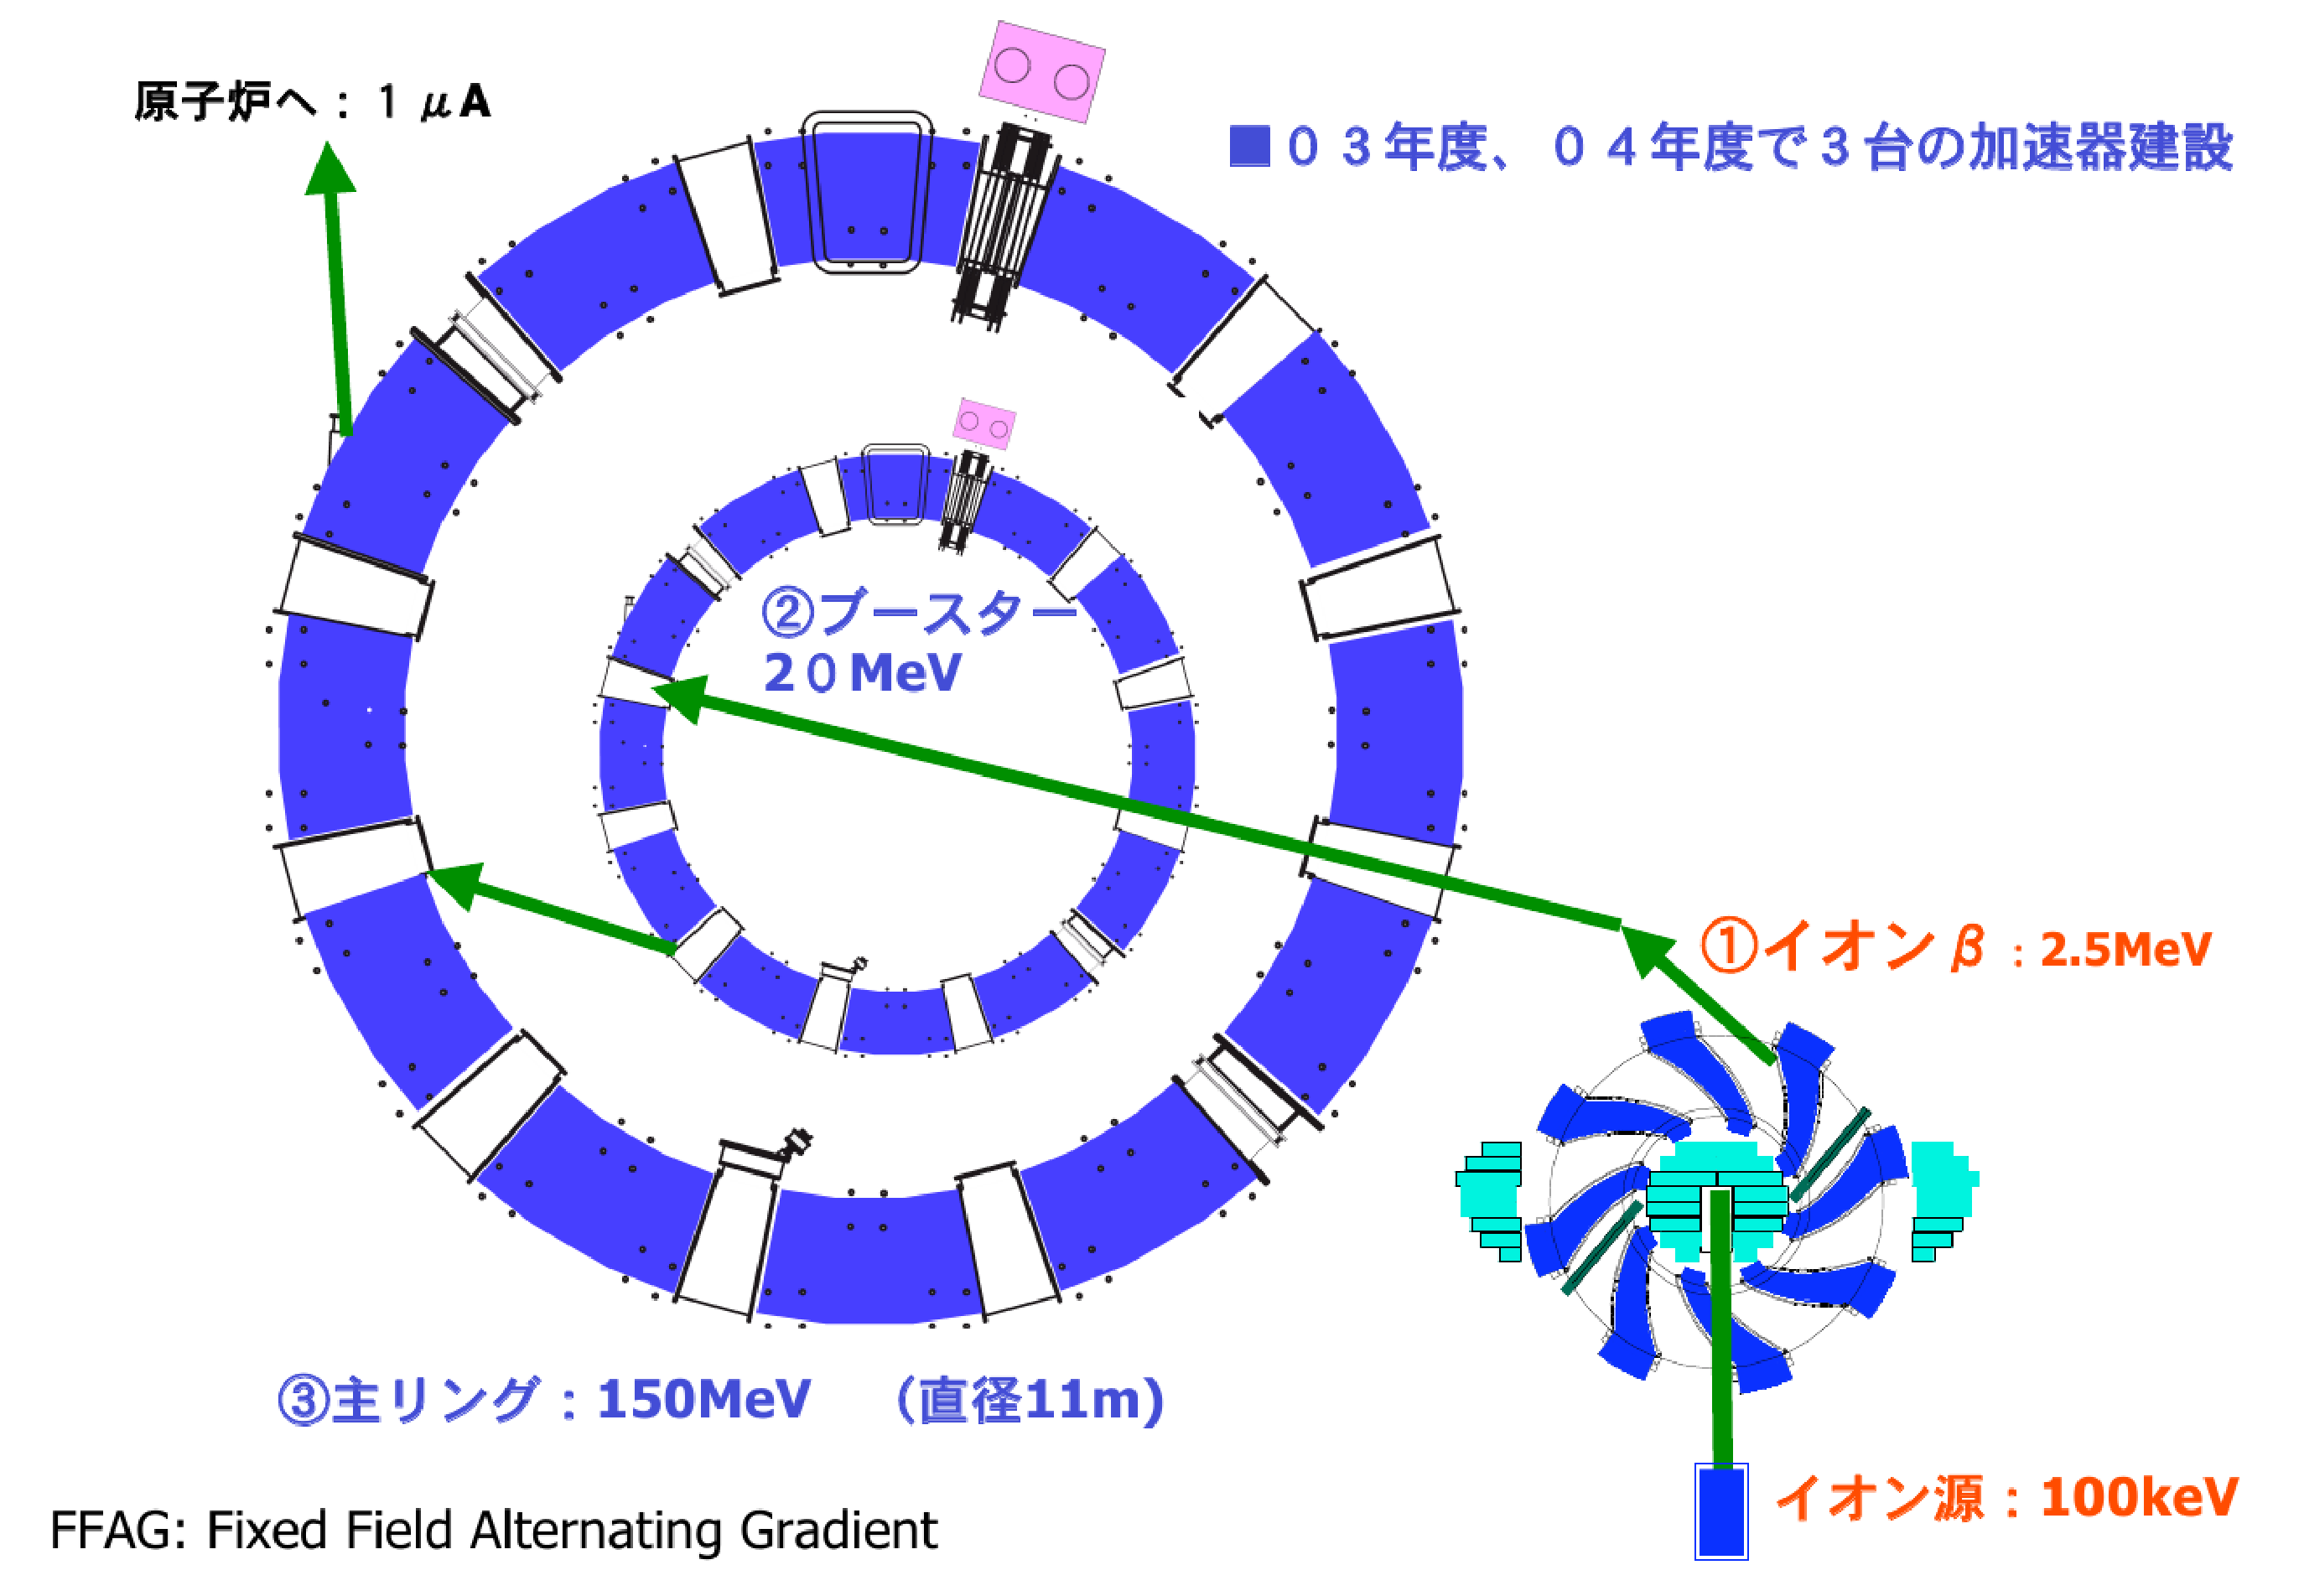
\includegraphics[width=.9\linewidth]{./figs_FFAG_introSlides/kurriCascadeSketch.eps}

\vspace{20mm}

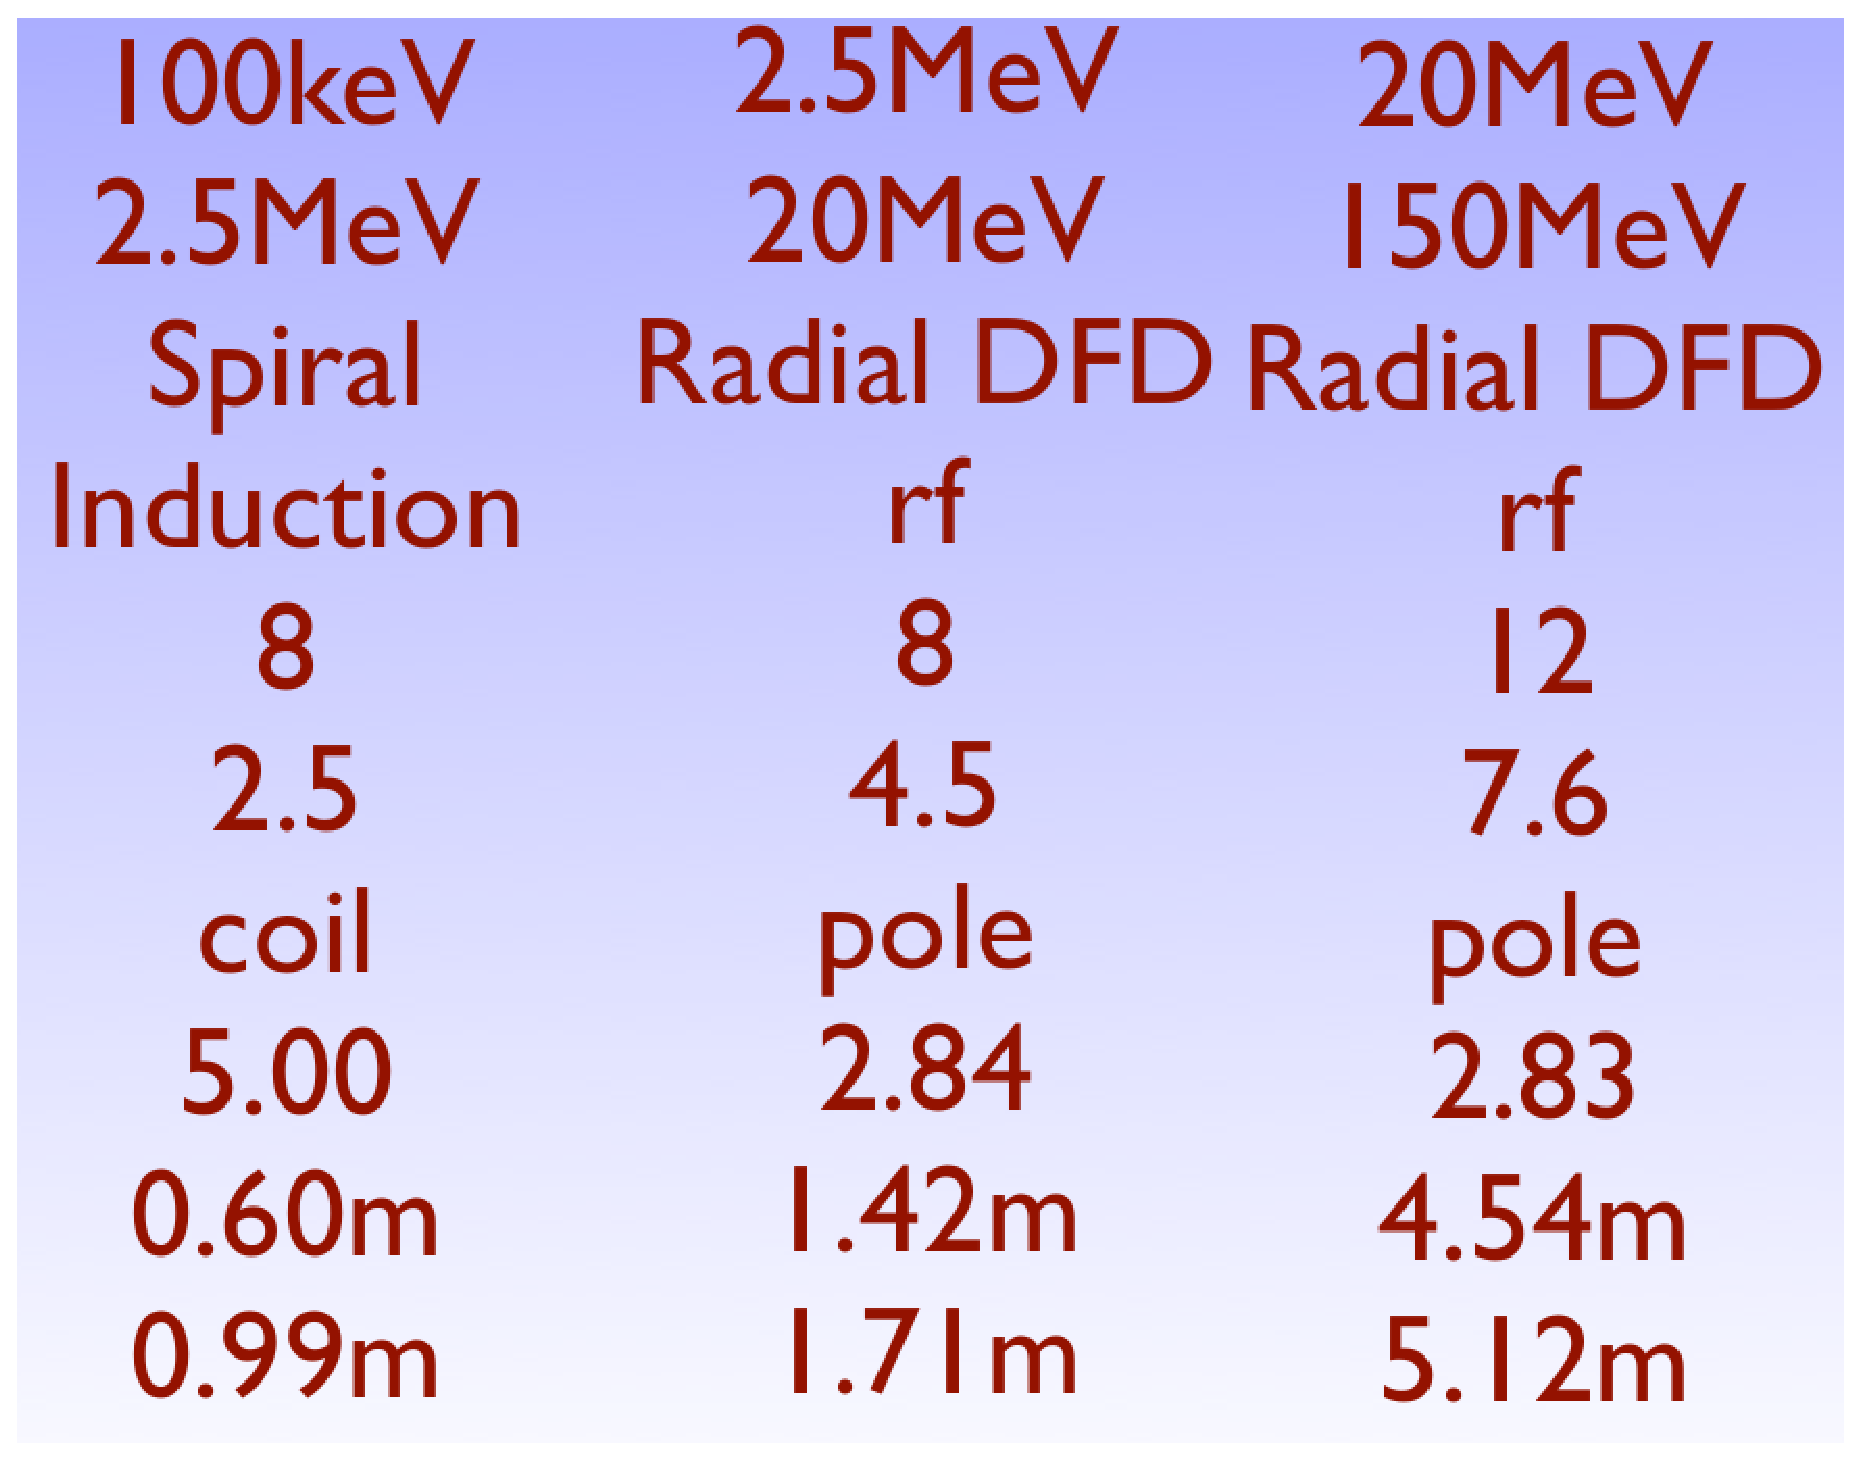
\includegraphics[width=.8\linewidth]{./figs_FFAG_introSlides/kurriCascadeParam.eps}

\end{minipage}\hspace{-15mm}
\begin{minipage}{.55\linewidth}
%\centering

\includegraphics[width=1.1\linewidth]{./figs_FFAG_introSlides/ionBeta.eps}

The magnet gap is non-scaling~: parallel faces. Pole face windings control the r-dependence of the vertical tune.

\end{minipage}



\end{minipage}





\clearpage 


\section{\LARGE ERIT}

{\fontsize{16}{20} \selectfont


\nib  ``Energy Recovery Internal Target'',  at KURRI, Kyoto University. 

~

\nid \black A compact proton storage ring for the production  of 10 MeV BNCT neutrons 

\nid \blue High neutron flux is needed at patient~: $\approx 2\, 10^{13}$neutrons in 30 minutes for typical tumor volume

\nid \black Today, a 5-10~MW reactor is used, there is needed for hospital environment compliant equipment~: ERIT

~

\begin{minipage}{.49\linewidth}
\blue Injector (425 MHz RFQ + IH-DTL)

\medskip

\black
H-,  kinetic energy 11 MeV

Peak/average beam current 5 mA / $>100\mu$A

Repetition rate 200 Hz, d.c. 2\%

~

\blue FFAG ring

\medskip

\black
FDF lattice, 8 cells

H- injection on internal Be target ($5-10\mu$m thick)

proton energy 11 MeV

circulating current 70 mA

~

\blue ERIT system

\medskip

\black
Beam survival 500-1000 turns

Target lifetime $>$ 1 month 

$\Delta$E / turn 70 keV
~

\blue RF cavity

\medskip

\black
Operated CW, 100 kW input power

RF voltage / frequency ~ ~ ~ 250 kV / 18.1 MHz

Harmonic number 5
\end{minipage}
\begin{minipage}{.49\linewidth}
\begin{center}

\includegraphics*[width=9.00cm]{./figs_FFAG_introSlides/KurriBNCT.eps}

~

\includegraphics*[width=.49\linewidth]{./figs_FFAG_introSlides/ERIT_sketch.eps}
\includegraphics*[width=.49\linewidth]{./figs_FFAG_introSlides/ERIT_Magnet.eps}

\end{center}
\end{minipage}

} %fontsize







\clearpage 

~

~ \\[-3ex]
\begin{minipage}{1.\linewidth}

\section{\LARGE PRISM }

\fontsize{15}{19} \selectfont

\nib A muon bunch phase rotator \\[1ex]
\begin{minipage}{.63\linewidth}


\nid An R/D program started in 2003

{\color{magenta}
 \nid {\bf FFAG used as phase rotator, for momentum compression}

\smallskip

 p=68MeV/c +/-20\% down to +/-2\% in 6 turns

\smallskip

 \noindent {\bf Advantage of FFAG optics~:  large geometrical acceptance, zero chromaticity}

 \nin A difficult task :   injection and extraction

}

\bigskip

\nid FFAG ring characteristics~: 

- DFD lattice ~ ~ ~ ~ 14t triplet yoke, 120 kW/triplet

% ring diam 10m. E=20MeV, 

- $K$, $B_F / B_D$  variable $\rightarrow$ quasi-decoupled $\nu_x$, $\nu_z$ adjustments

- H / V apertures : ~ ~ 1 / 0.3~m 

- acceptance : ~ ~  4 $\pi$~cm.rad $\times$ 0.65~$\pi$~cm.rad

- RF :  ~ ~ 5-gap cavity, 33 cm gap, 150-200 kV/m, 2MV/turn, saw-tooth waveform

%  \begin{center}
%      \rule{30mm}{.1mm}
%  \end{center}
\begin{center}
\mbox{
\includegraphics*[bbllx=20,bblly=100,bburx=567,bbury=480,width=6.00cm]{./figs_FFAG_introSlides/prism_phase-dp.eps} ~ ~ 
\includegraphics*[bbllx=20,bblly=100,bburx=567,bbury=480,width=6.00cm]{./figs_FFAG_introSlides/prism_x-pass.eps}
}
\end{center}


{\color{blue}
\nid 2005: downsized to 6 cells for POP, \\
- central orbit radius 3~meter \\
-2.1 MHz (h=5) RF, gap voltage 33 kV peak \\
- operated using 100~MeV/c alphas from an $\rm ^{241}$Am source.

}


\end{minipage}\hspace{10mm}
\begin{minipage}{.36\linewidth}


\begin{center}

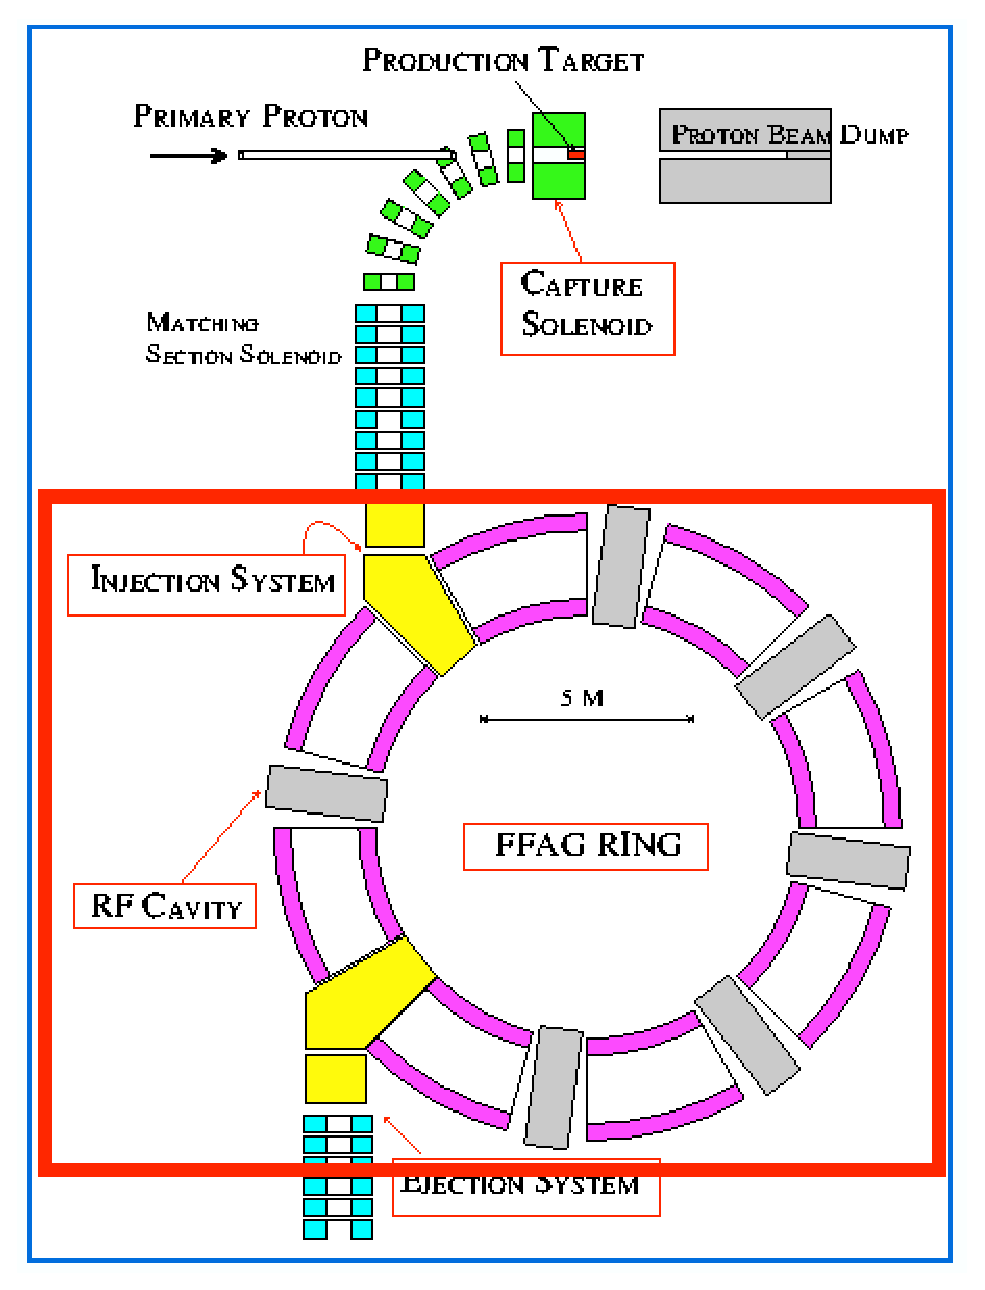
\includegraphics[width=7.00cm]{./figs_FFAG_introSlides/prism_ring.eps}

\mbox{\hspace{-10mm}
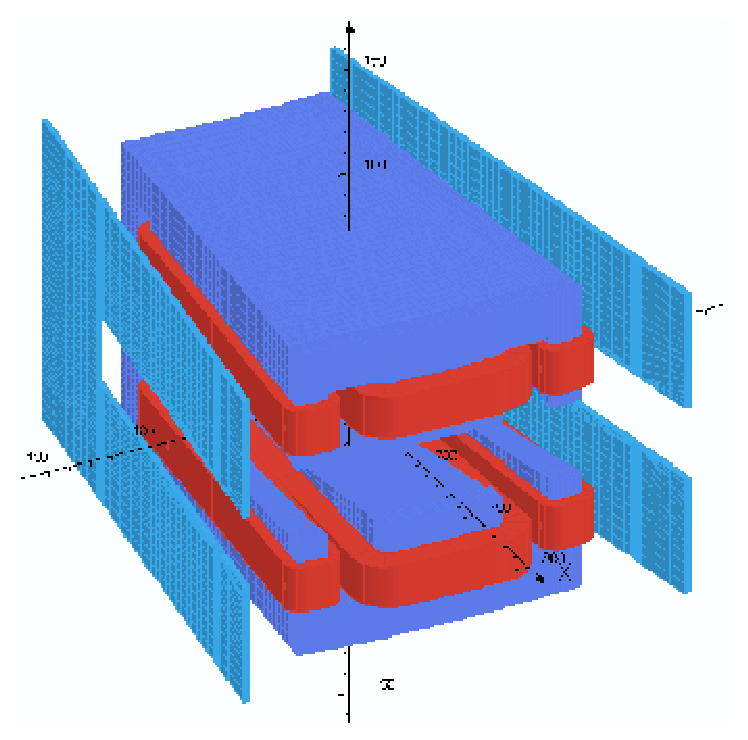
\includegraphics[width=5.00cm]{./figs_FFAG_introSlides/prism_mag.eps}
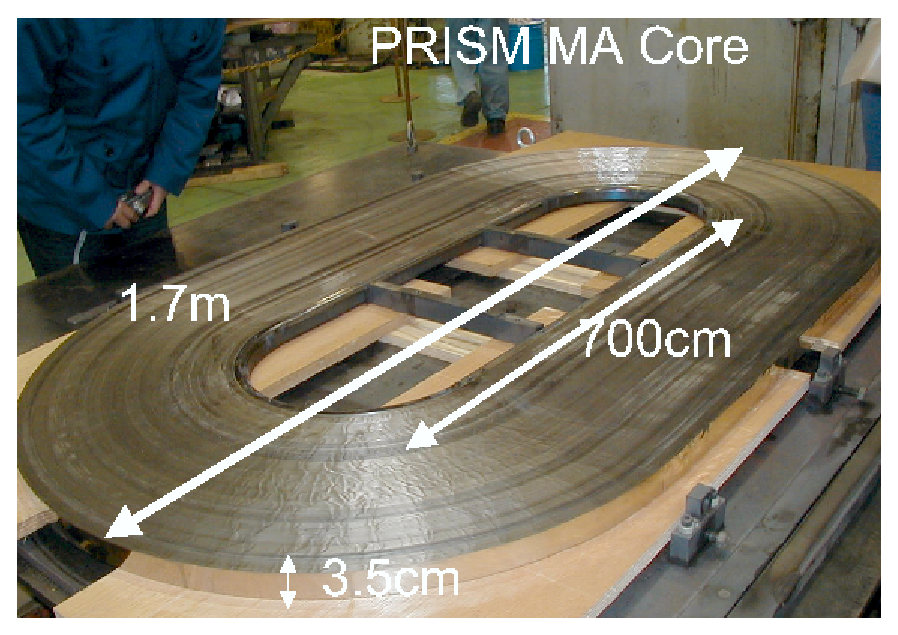
\includegraphics[width=5.00cm]{./figs_FFAG_introSlides/prism_RFcore.eps}
}


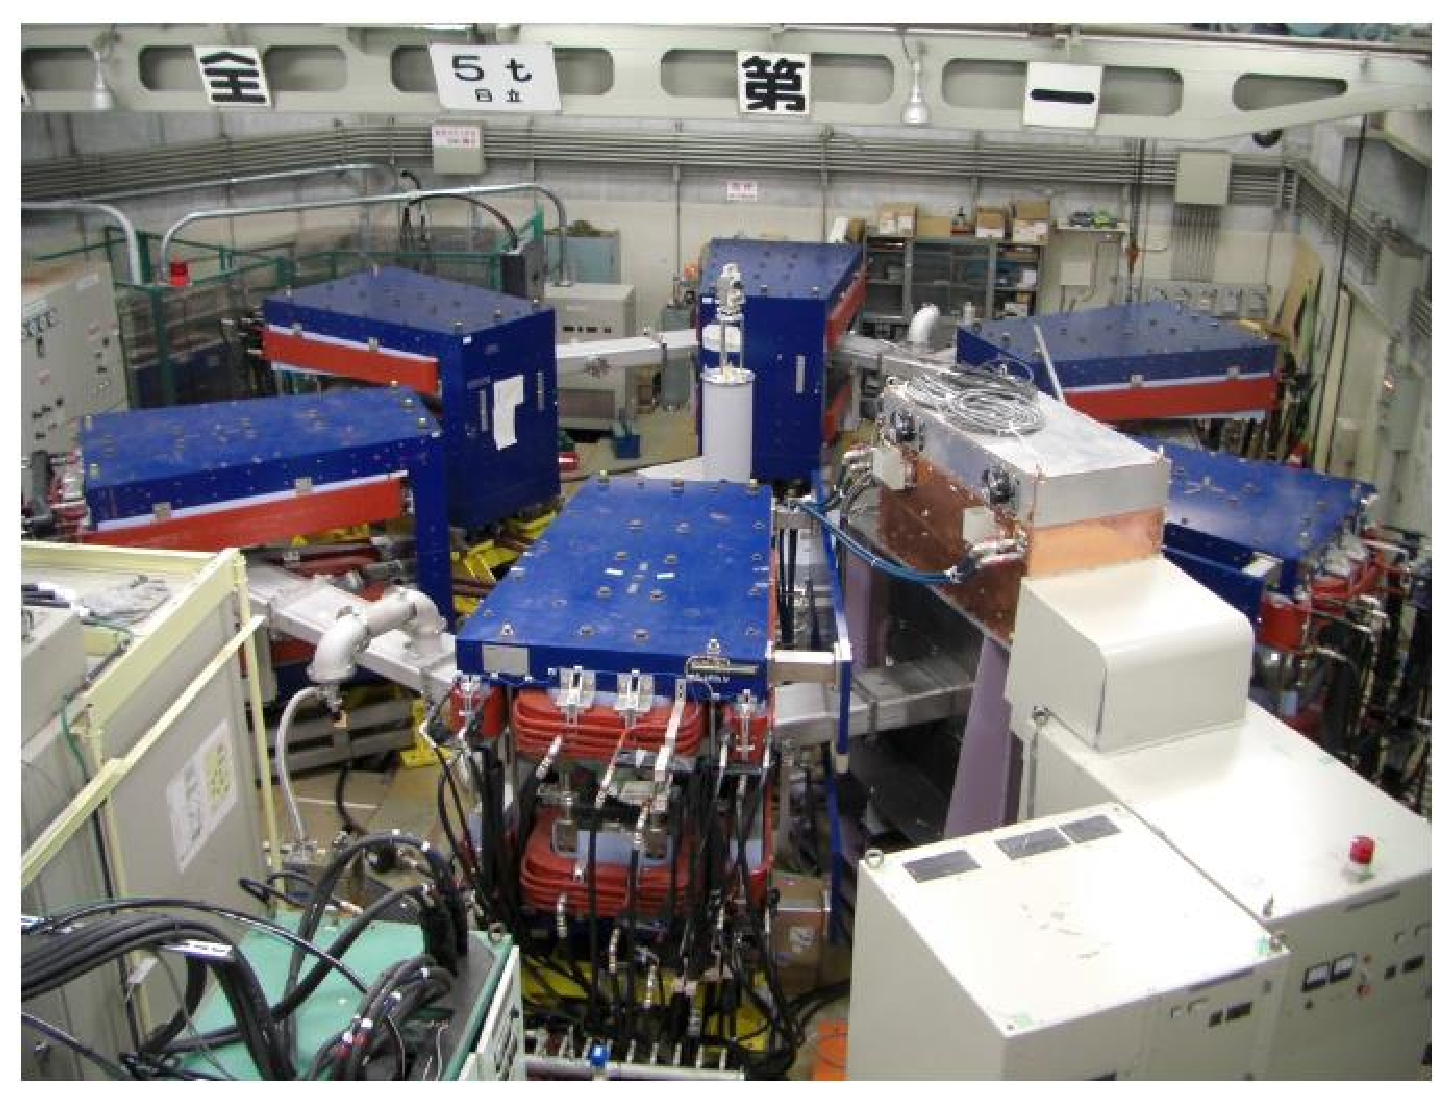
\includegraphics[width=5.00cm]{./figs_FFAG_introSlides/prismRing.eps}

\end{center}

\end{minipage}
\end{minipage}





\clearpage 

\section{\LARGE RACCAM }


{\Large \bf
\black
\nib Working frame : Neutrino factory R/D and medical applications. 

French ANR funding, 2006-2008. %,  3.5~MEU cost \\[.7ex]

\blue 
\nib A feasibility study of a rapid-cycling, variable energy, spiral lattice scaling FFAG \\[.7ex]
\black
\nib Magnet prototype (built by SIGMAPHI) proved $\left\{ \begin{array}{l} \textbf{gap shaping spiral sector} \\
\textbf{scaling FFAG field, including flutter}  \end{array} \right.$ \\[.7ex]

\nin Tracking in measured field maps (3D Hall-probe, by SIGMAPHI) proved $\left\{ \begin{array}{l}  
\textbf{constant tunes} \\ \textbf{large dynamical aperture} \end{array} \right.$ \\[.7ex]

\black
\nib Outcome~: 

- demonstration of gap shaping scaling spiral \\
 dipole feasibility. {\blue First of the kind}.

- a cost-effective multiple-beam delivery \\
hadrontherapy installation. 

\vspace{-1ex}
\mbox{
\begin{minipage}{.5\linewidth}
\centering

 \includegraphics*[width=.7\linewidth]{./figs_FFAG_introSlides/08-10-29_Ring5Xtractions-3D.eps}

\end{minipage}\hspace{-0ex}
\begin{minipage}{.6\linewidth}
\centering

~

\vspace{-10ex}
\begin{minipage}{.99\linewidth}

\begin{minipage}{.5\linewidth}

\hspace{6ex} \includegraphics*[width=.99\linewidth]{./figs_FFAG_introSlides/raccamMagnet.eps}

\end{minipage}

\begin{minipage}{.5\linewidth}

\hspace{-0ex}
\mbox{
 \includegraphics*[width=.8\linewidth]{./figs_FFAG_introSlides/raccamTunes.eps}
 \includegraphics*[bbllx=20,bblly=20,bburx=567,bbury=457,width=.9\linewidth]{./figs_FFAG_introSlides/raccamDA.eps}
}

\end{minipage}
\end{minipage}
\end{minipage}
}

%\blue 
%\nib Magnet design was further exploited in KURRI-KUCA 700~MeV upgrade project 

%\clearpage 
%\section{\LARGE RACCAM}
%\nib FFAG R\&D, NuFact sector, application to protontherapy
%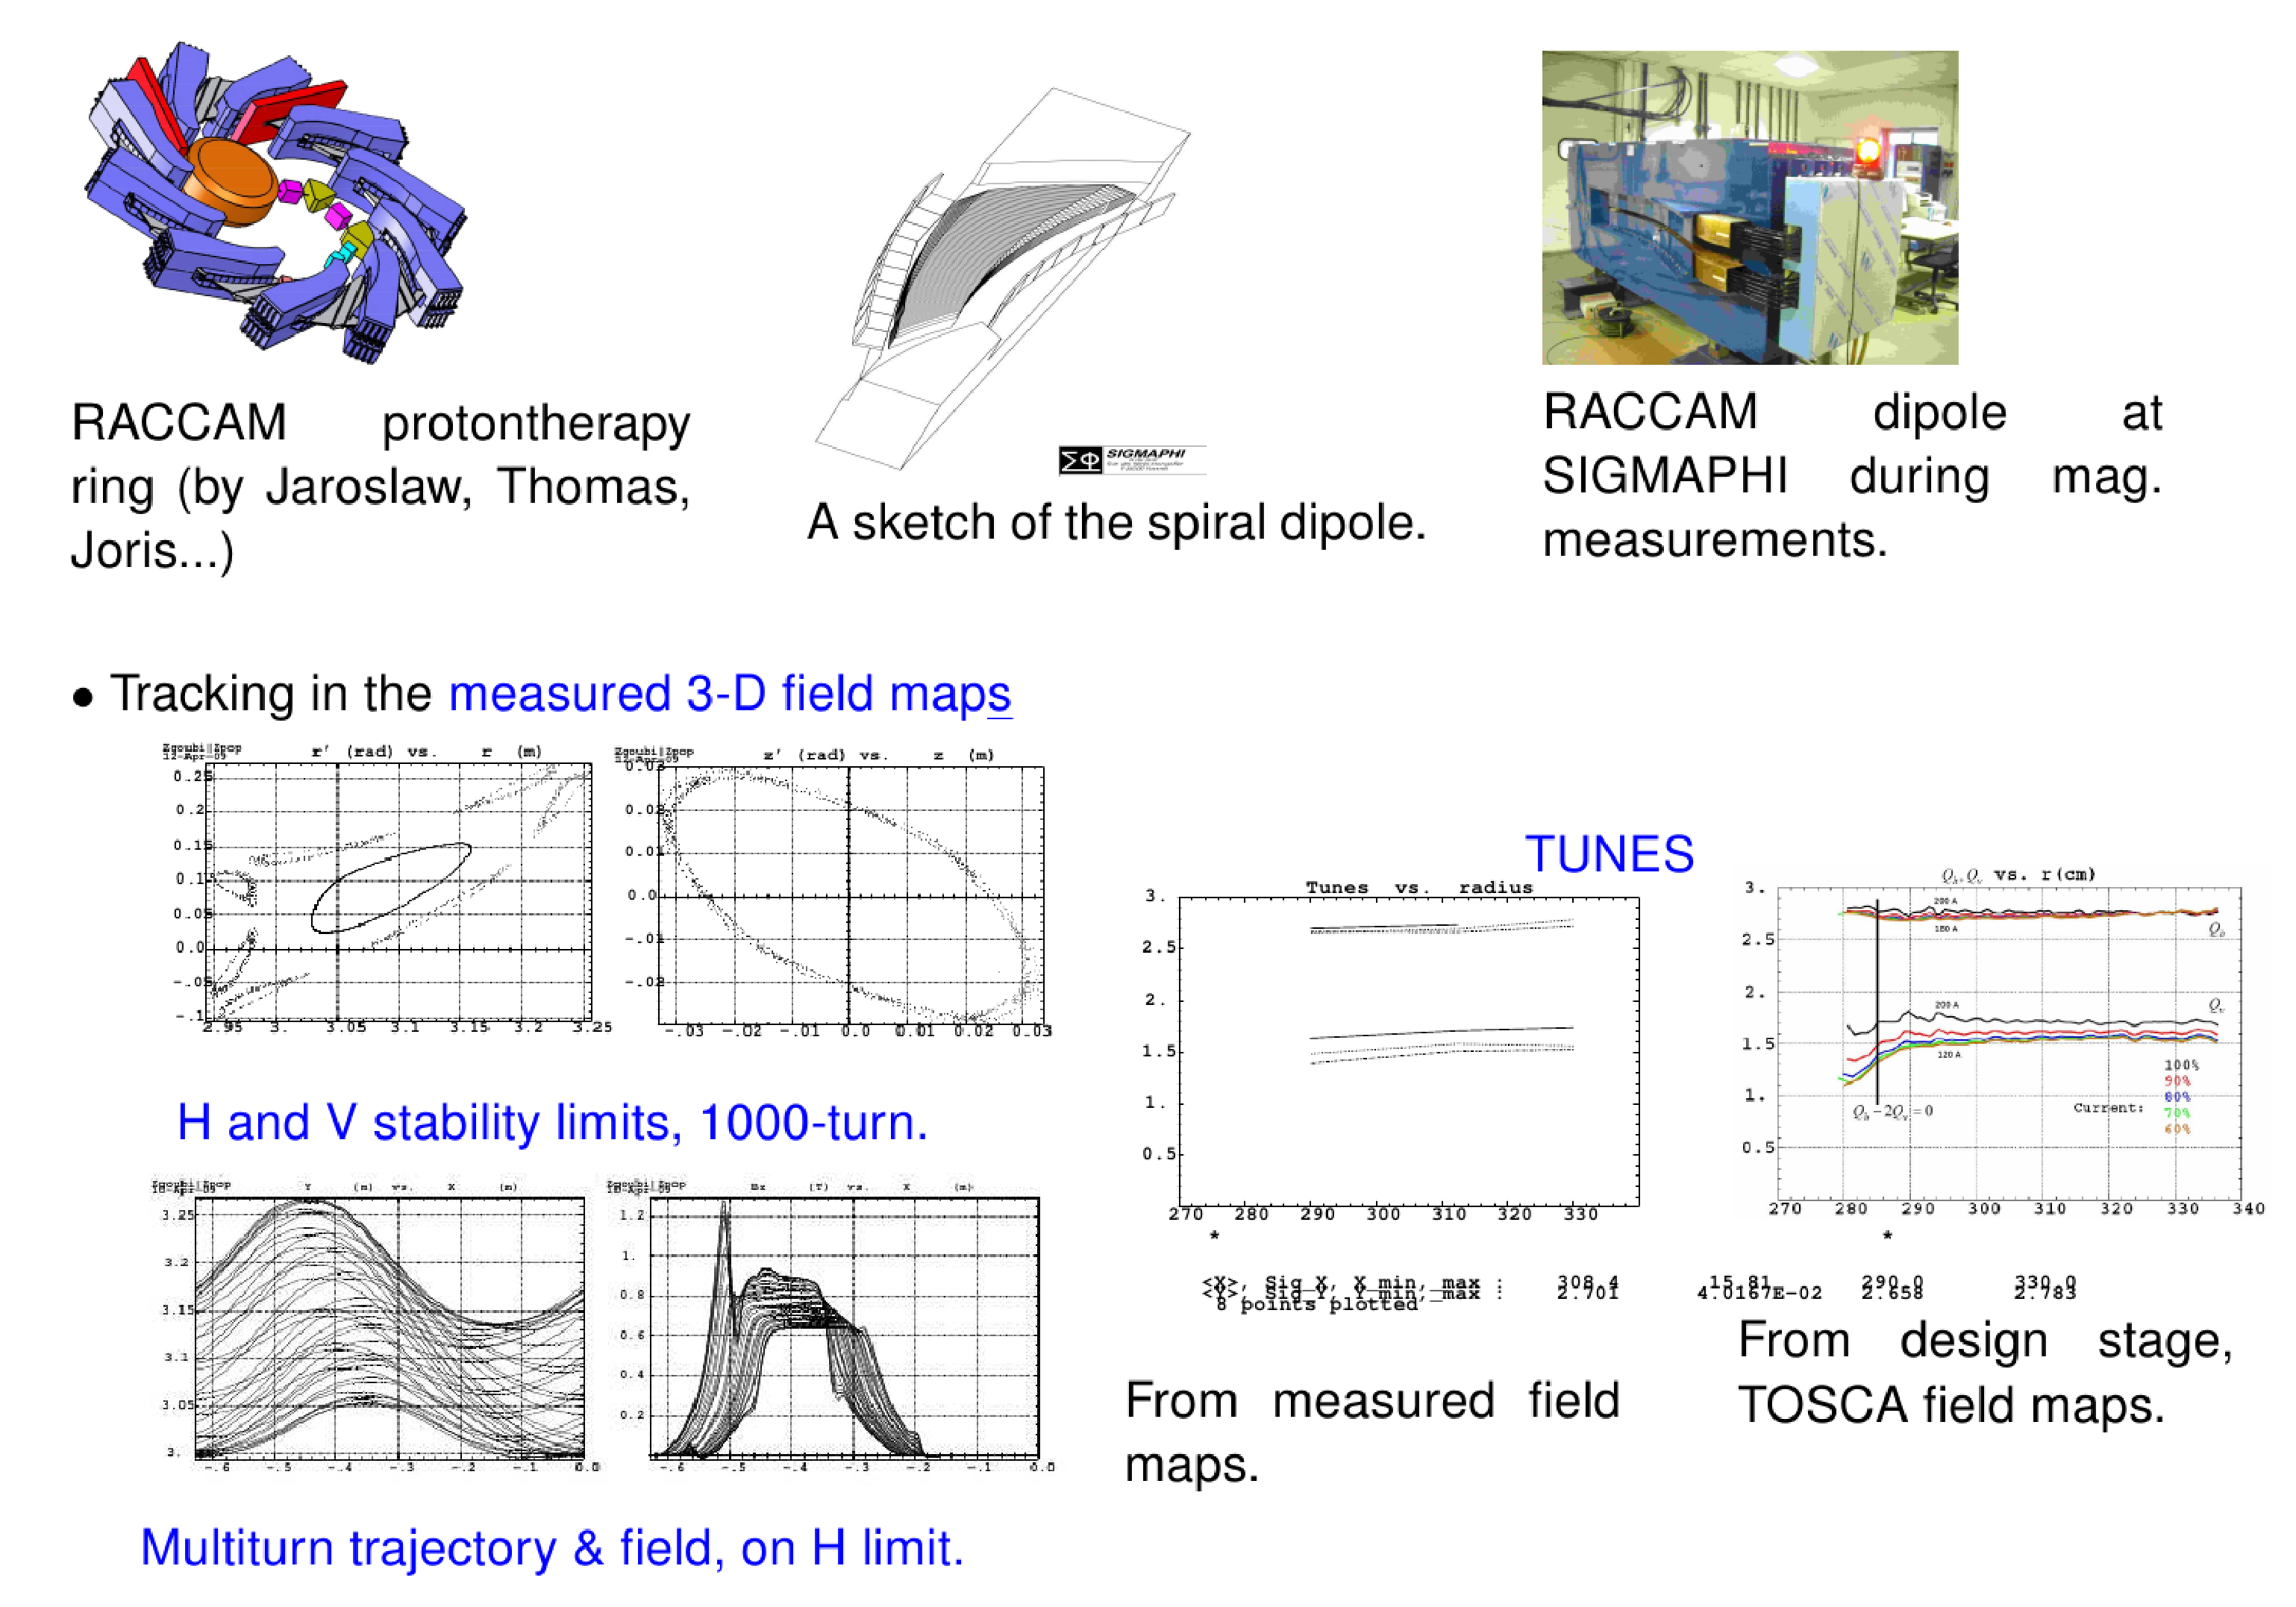
\includegraphics[width=1.\linewidth]{./figs_FFAG_introSlides/raccam.eps}

}


\clearpage 


{\fontsize{17}{20} \selectfont

\section{\LARGE Straight S-FFAG line}

\nid Scaling FFAG accelerators can be designed not only in a ring shape, but also with no overall bend. 

\nid This requires a mid-plane guide field of the form 
$$B_y(x,s) = B_0 e^{m(x - x_0 )} F(s)$$
\nid Similarly to the cylindrical $(r,\theta)$ case, $B_0$ is some reference field value, taken at some arbitrary 
reference $x_0$, $F(s)$ is a flutter function.
% \frac{\textstyle{}}{\textstyle{}} 

$m= \frac{\textstyle{\rho}}{\textstyle{B\rho}} \frac{\textstyle{\partial B}}{\textstyle{\partial x}} $
is the normalized field gradient.

The experiment used the 11~MeV linac (injector of the 150 MeV FFAG). The FDF cell is moved horizontally (bellows) to match the 
incident beam momentum to the proper FFAG orbit. 

The experiment measured the orbit location, optical functions including phase advances, for various momenta, and showed 
good agreement with  outcomes of tracking in field maps. \\
\mbox{
\begin{minipage}{.49\linewidth}
\centering
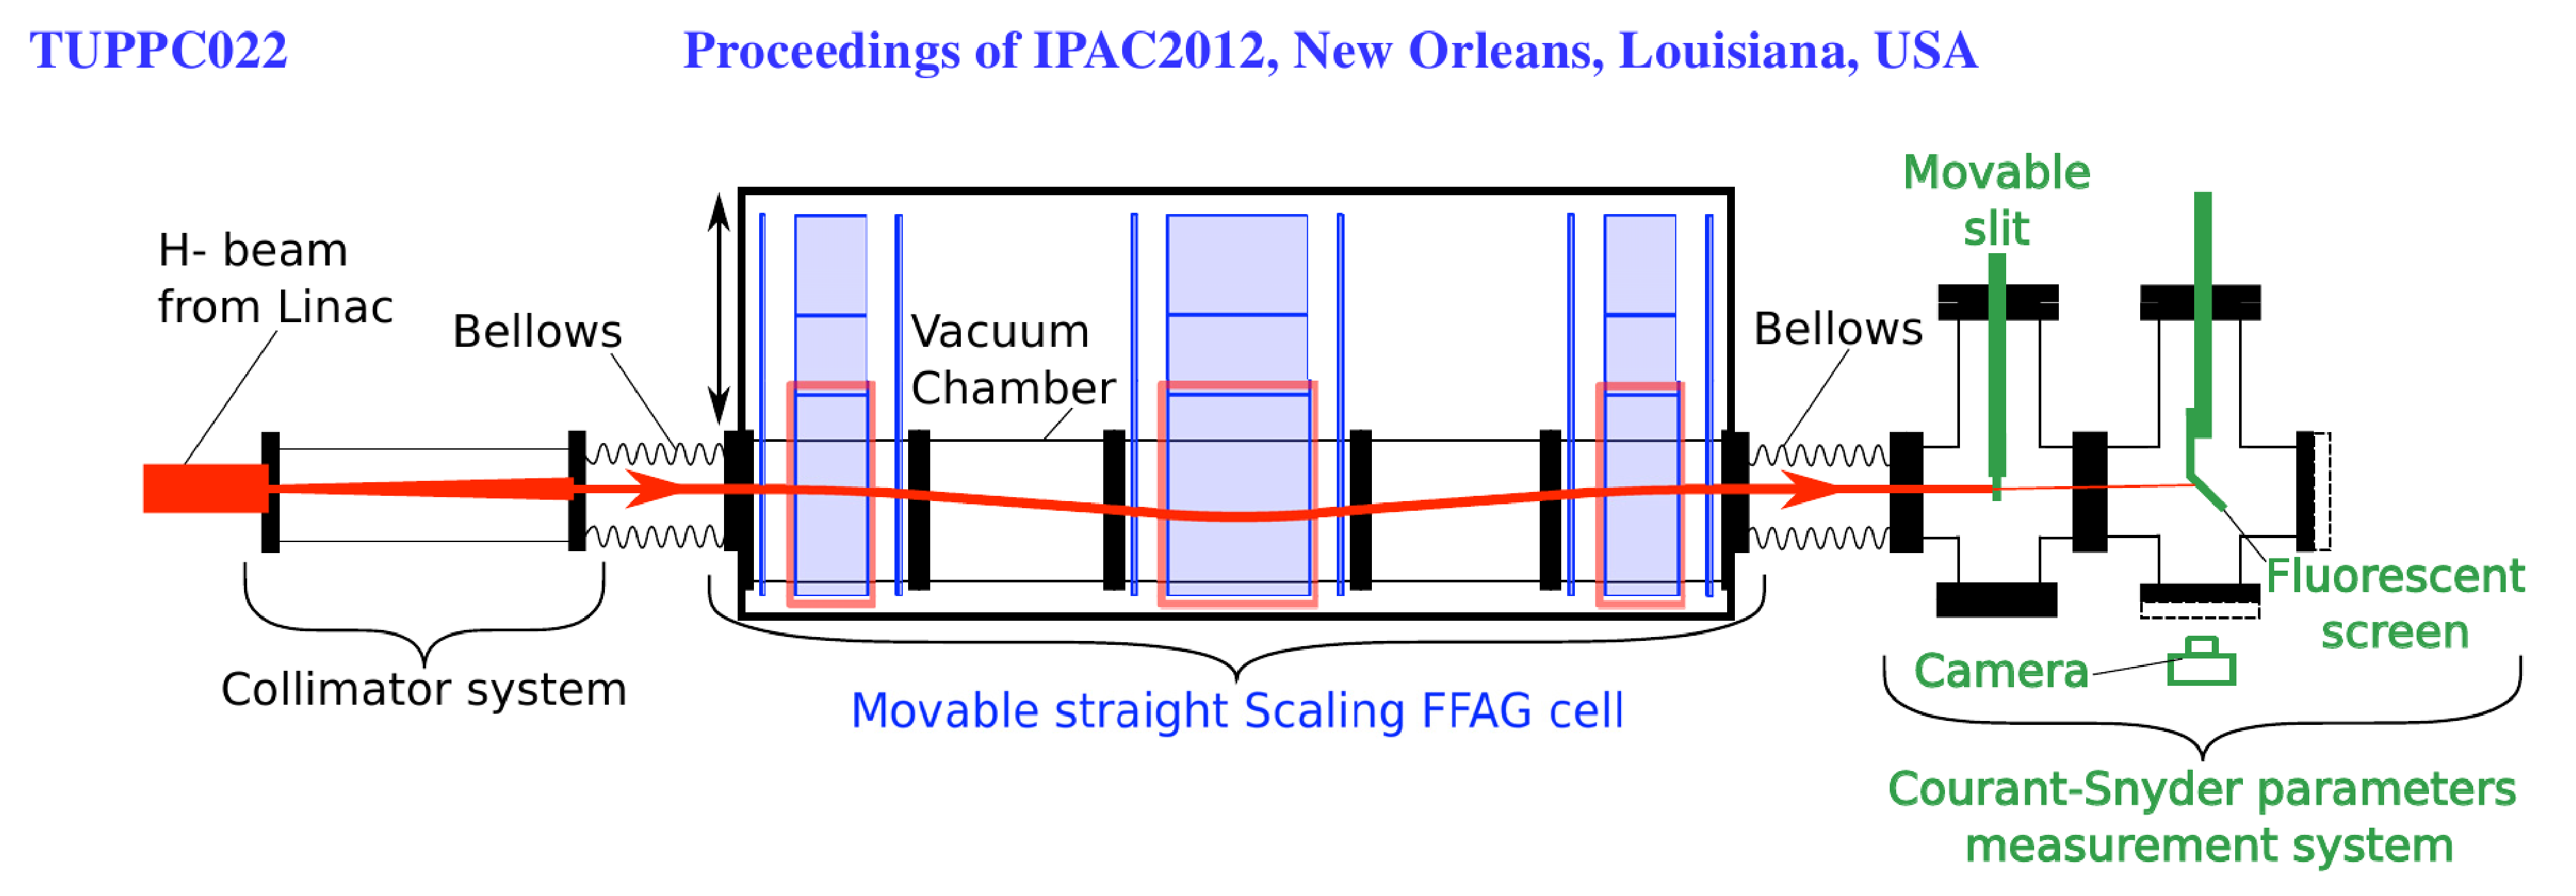
\includegraphics[width=1.3\linewidth]{./figs_FFAG_introSlides/FFAGBLineJBL.eps}

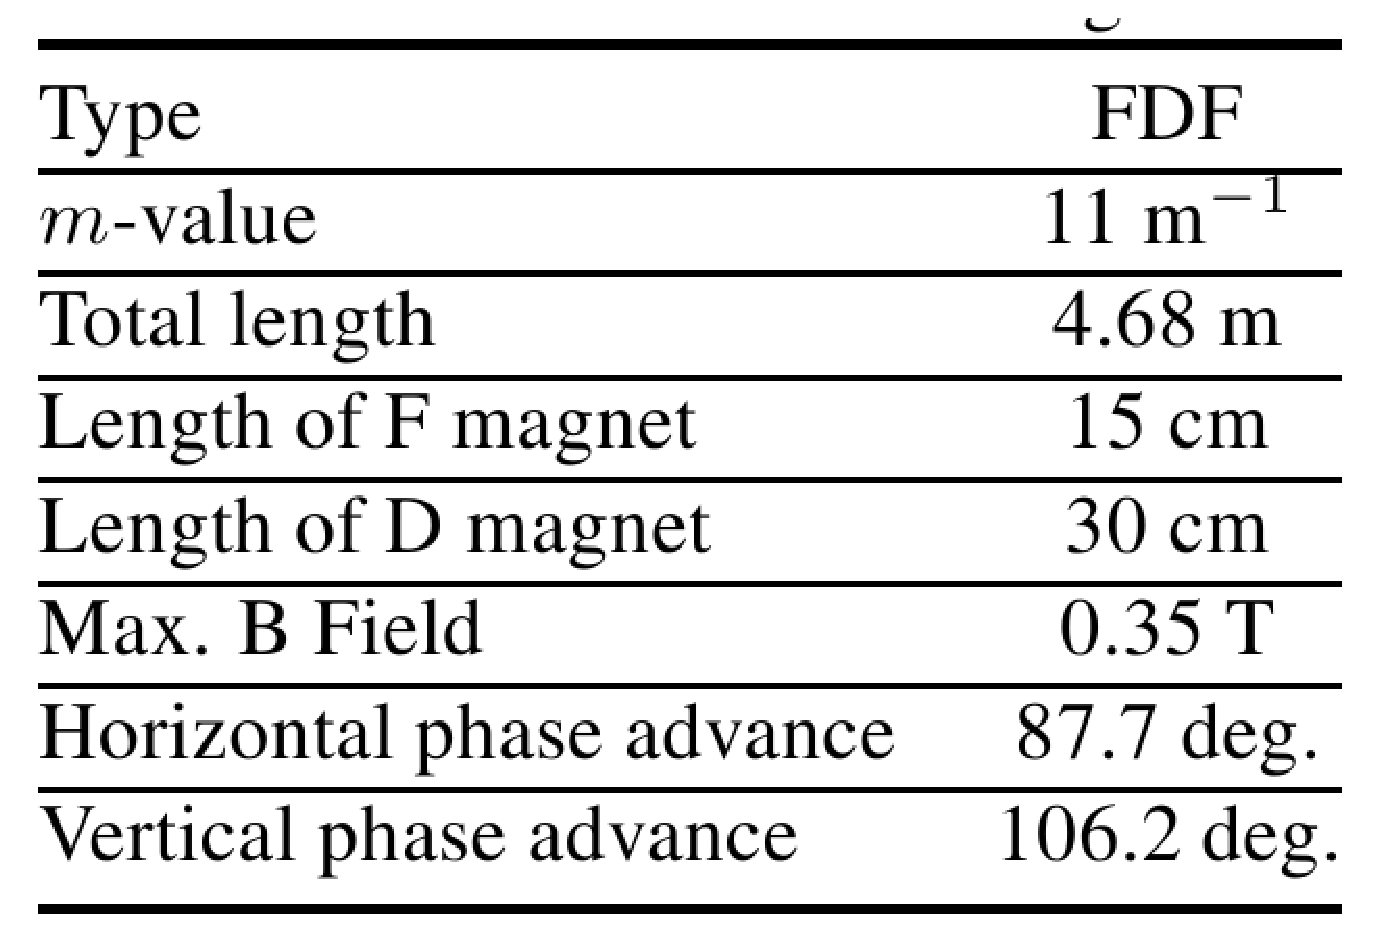
\includegraphics[width=.5\linewidth]{./figs_FFAG_introSlides/FFAGBLineJBL_param.eps} ~ ~ ~ ~ 

\end{minipage}\hspace{4ex}
\begin{minipage}{.49\linewidth}
\centering

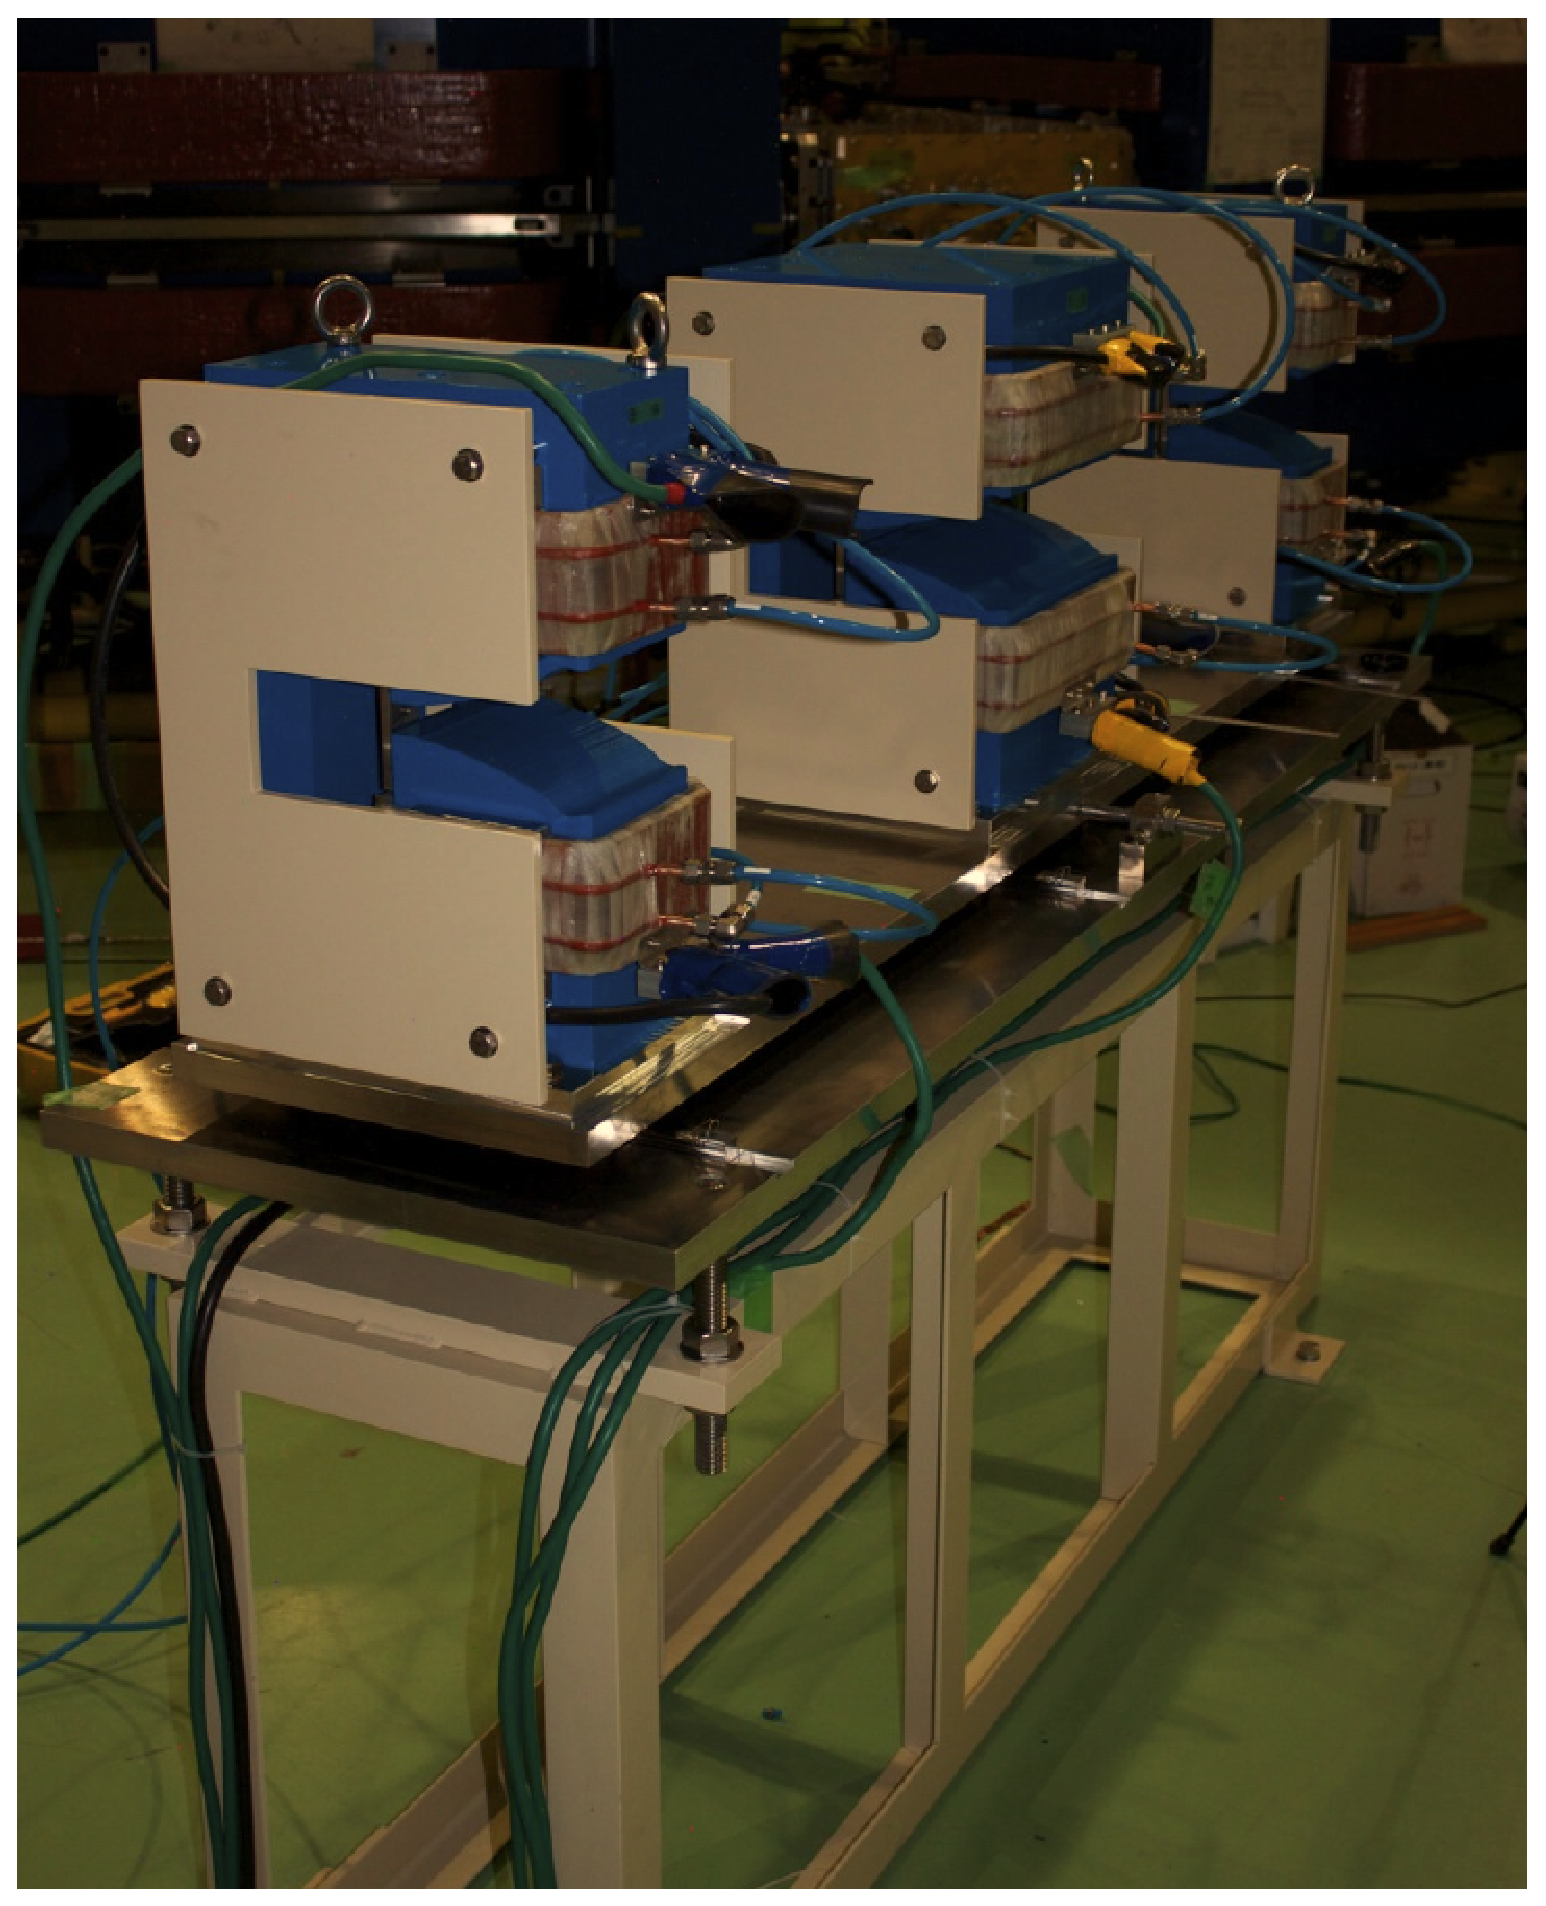
\includegraphics[width=.6\linewidth]{./figs_FFAG_introSlides/FFAGBLineJBL_photo.eps}


\end{minipage}\hspace{1mm}
}
}

\clearpage 


\section{\LARGE EMMA }


%\addcontentsline{toc}{subsection}{\numberline{}\Large  A new concept~: non-scaling FFAG}
\subsection*{\LARGE Back to the neutrino factory,  US-Study-2a~: based on linear  FFAG}


\large   

\begin{minipage}[t]{.63\linewidth}


\large   


\noindent - FFAG  based on linear optical elements (quadrupoles) 

\noindent - orbits no longer scale, tunes  are allowed to  vary with energy  

~

~

~

This has a series of consequences~: 

~

\blue   $\bullet$  $R/\rho<2$ - this decreases the machine size compared to classical (scaling) FFAG


~

\black   $\bullet$ horizontal beam excursion is reasonable (small $D_x$) \\
$\rightarrow$ {\bf magnets apertures are much  smaller }

~

\blue   $\bullet$ yields {\bf large transverse acceptance }  $\leftarrow$ fields are linear ($3\pi$cm achieved) 

~

\black   $\bullet$ small $\delta$TOF over  energy span, allows {\bf fast acceleration } 
 high gradient RF (200~MHz type SCRF cavities)

~

\blue  $\bullet$  Above 5~GeV, non-scaling linear  FFAG  method yields  {\bf lower cost/GeV than RLA}. 

\black 




\end{minipage}\hspace{0mm}
\begin{minipage}[t]{.4\linewidth}

\vspace{-9mm}


\begin{center}

\includegraphics*[width=10.00cm]{./figs_FFAG_introSlides/feb17-study2a-schematics2.eps}

\includegraphics*[width=10.00cm]{./figs_FFAG_introSlides/RFCryostat.eps}

\end{center}

\end{minipage}\hspace{0mm}




\clearpage

\vspace{-10mm}

{\bf \LARGE \blue $\bullet$ The EMMA experiment. }

{\Large \nid An experimental  model to investigate the new concept of ``linear FFAG''~: 

\medskip

 - linear magnets (quadrupoles) \red $\longrightarrow$ yields huge acceptance \black

 - fixed field  \red $\longrightarrow$ yields fast acceleration 

 - fast acceleration \red $\longrightarrow$ requires a lot of RF, and fixed frequency, gutter acceleration 

\black
}


\begin{minipage}[c]{0.38\linewidth}
\vspace{1ex}
  \begin{center}

  \includegraphics*[width=11.00cm]{./figs_FFAG_introSlides/emmaRing.eps}

\it
A model of Study IIa FFAG 

\vspace{-.4ex}
10 to 20 MeV 

\vspace{-.4ex}
 42 cells, doublet

\vspace{-.4ex}
 pole-tip $fields ~ \approx 0.2$~T

\vspace{-.4ex}
 apertures $\approx \phi40$~mm

\vspace{-.4ex}
 37cm cell length 

\vspace{-.4ex}
 ~16m circumference 

\vspace{-.4ex}
 1.3GHz  RF

\vspace{-.4ex}  
 1 cavity every other cell 
  \end{center}
\end{minipage} ~ ~ ~ ~ ~ ~ 
\begin{minipage}[c]{0.5\linewidth}
  \begin{center}
  \includegraphics*[width=13.00cm]{./figs_FFAG_introSlides/emmaPage.eps}
  \end{center}
\end{minipage}



\clearpage


\begin{minipage}{.5\linewidth}

{\Large \blue \bf
\noindent
\nib Construction at Daresbury Lab.  started in 2007 \\[1ex]
\nib Commissioning started in 2010 \\[1ex]
\nib ``Serpentine'' acceleration demonstrated in 2011 \\[1ex]
}


\hspace{-10mm}
\includegraphics*[width=15cm]{./figs_FFAG_introSlides/EMMA_lowResol.eps}

\end{minipage}\hfill
\begin{minipage}{.3499\linewidth}

\fbox{
\begin{minipage}{1.\linewidth}

\fbox{\bf \LARGE EMMA parameters} 

\large 
\begin{tabular}{lcccl}
\bf Energy range            &\it \blue MeV &    10 - 20    \\
\bf number of turns    &        &    $<$16    \\
\bf circumference      &\it \blue  m  &       16.568       &   \\
\bf Lattice           &        &     F/D doublet ~ ~  \\
\bf No of cells      &  &     42       &   \\[.5ex]
\bf RF frequency       &\it \blue GHz  &      1.3        &  \\
\bf No of cavities     &  &    19        &   \\
\bf RF voltage    &\it \blue kV/cav.  &   20 - 120   &   \\
\bf RF power           &\it \blue kW/cav.  &      $<$2  \\[.5ex]
%\bf Bunch emittance   &\it \blue $\pi mm$  &    3  \\
%\bf Bunch charge   &\it \blue $pC/\mu A$  &    $<$32   \\
\bf Rep. rate           &\it \blue Hz  &  1-20  \\
\end{tabular}


\end{minipage}
}

~

~


\begin{minipage}{1.\linewidth}
\centering

\includegraphics*[width=.99\linewidth]{./figs_FFAG_introSlides/serpentMeas.eps}

%\includegraphics*[bbllx=20,bblly=100,bburx=567,bbury=480,width=.65\linewidth]{./figs_FFAG_introSlides/tof.eps}

%\includegraphics*[bbllx=20,bblly=100,bburx=567,bbury=480,width=.65\linewidth]{./figs_FFAG_introSlides/phaseEnr_06.eps}


\end{minipage}
\end{minipage}




\clearpage 

\Large 

\section{\LARGE A bestiary of FFAG design studies  }

 A *very limited* excerpt of what can be found in our Labs... See the bibliography for more, in particular the FFAG workshops.

~

{\fontsize{17}{24} \selectfont

 {\bf \blue \nib
nuSTORM FFAG decay ring, J.-B. Lagrange et al. [IPAC2016]
}

~

\nid Neutrinos from STORed Muon  beam (nuSTORM), the simplest implementation of a neutrino factory~:
 pions are directly injected into a racetrack storage ring, where the circulating muon beam is captured. 

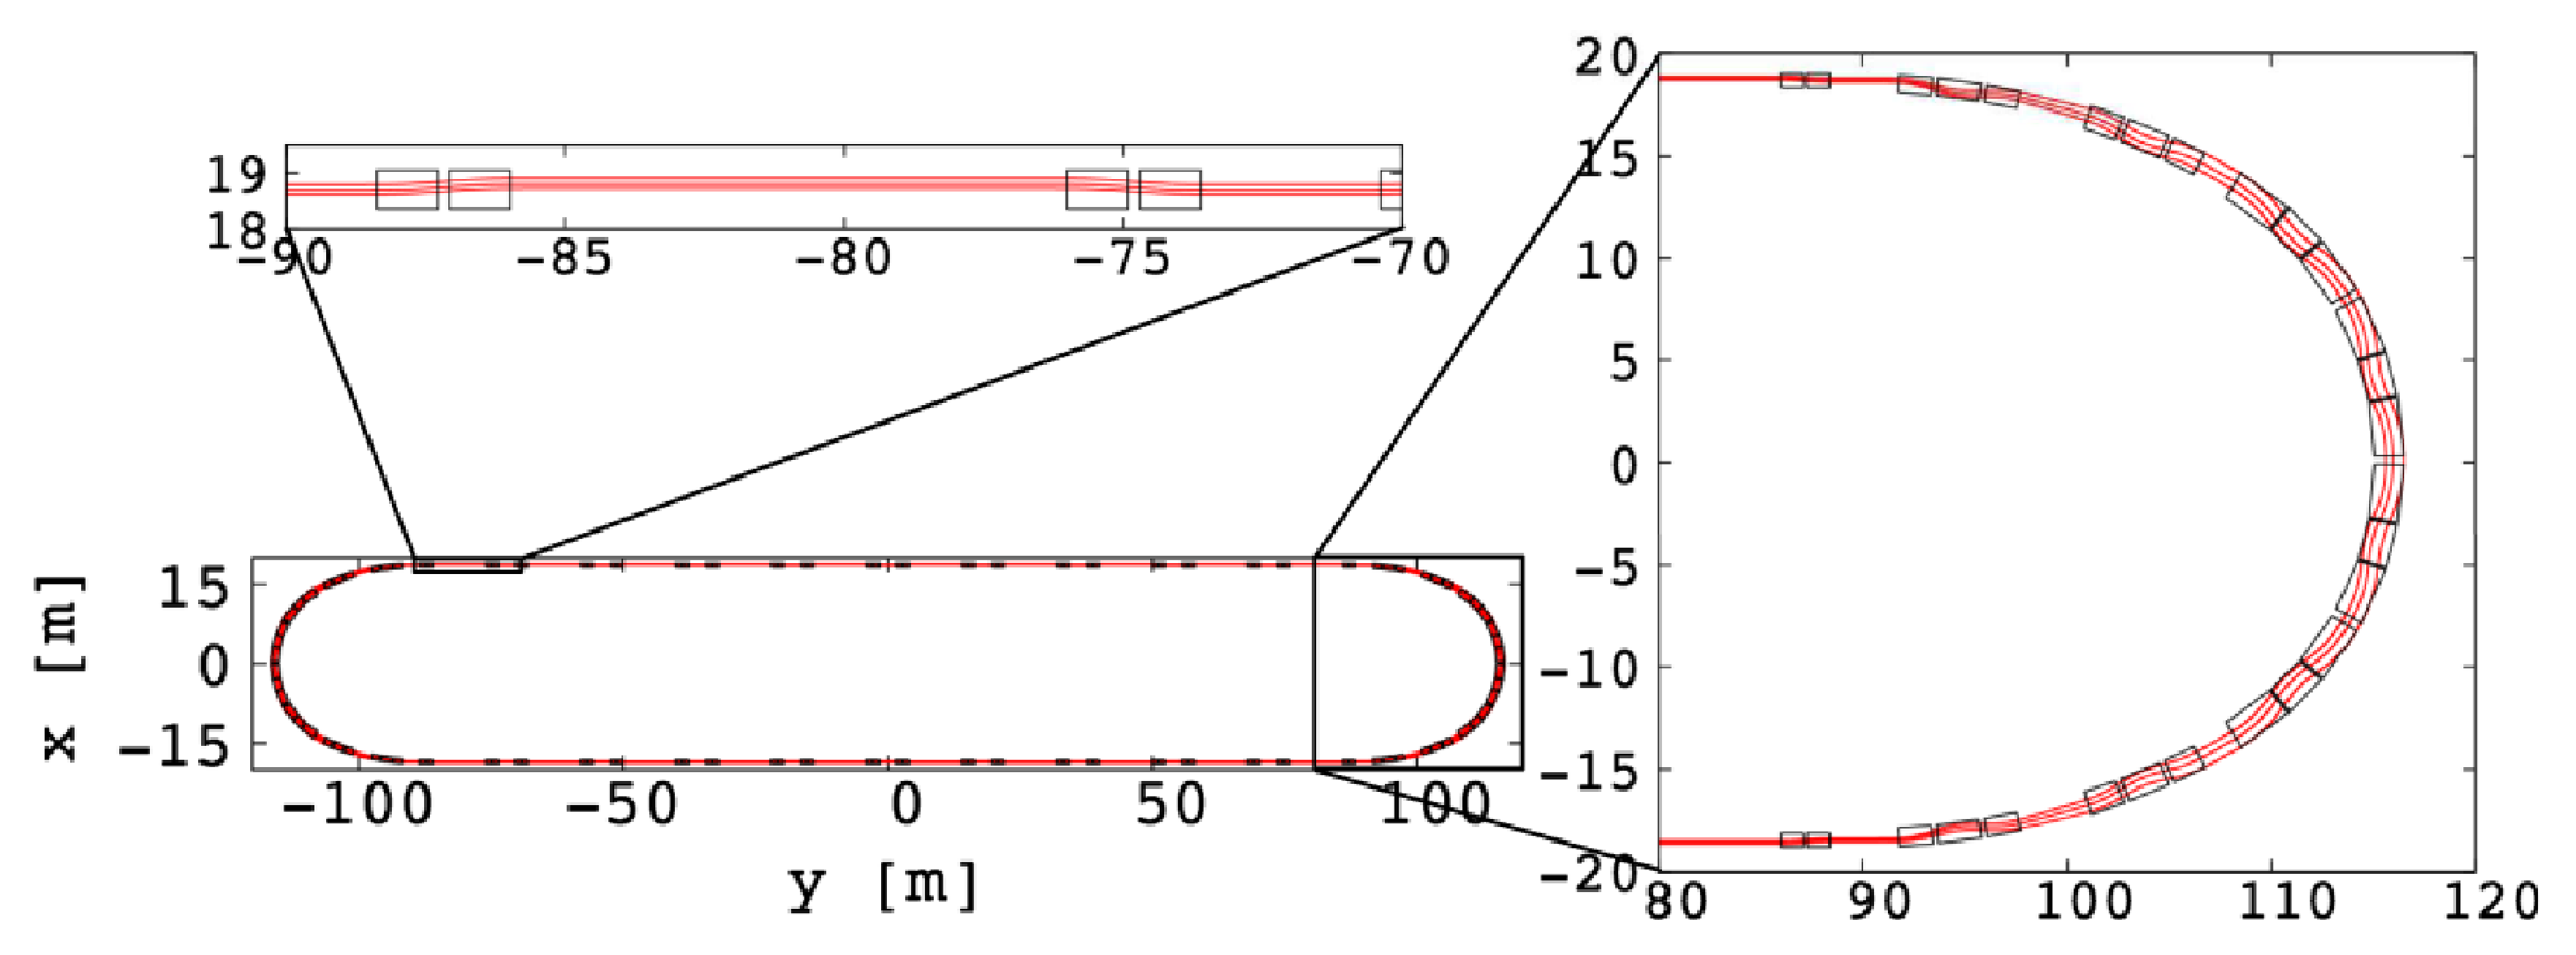
\includegraphics[width=.75\linewidth]{./figs_FFAG_introSlides/nuStorm.eps} 

\textsl{ ~ \\
\nid The racetrack nuSTORM FFAG lattice with  zoom on the straight section (top left)
and  on the arc section (right). \\
\nid The muon flux  is  key to successful
neutrino experiment, so, FFAG optics allows ring with large momentum
 acceptance,  $\sim \pm 20$\%. \\
 straight section to avoid activation in the arc. 
}

}%fontsize  


\clearpage

{\fontsize{17}{24} \selectfont

\nib {\bf \blue
Vertical FFAG [S.~Brooks, PRST AB 16, 084001 (2013)]
}



\black 

\nid Vertical scaling optics  was devised by K.~Ohkawa (once known as the ``smokatron''), 



\blue

\medskip

\nid Re-investigated recently [S. Brooks, prst-ab]

\vspace{1ex}

\black

\centering
\begin{minipage}{.99\linewidth}
\centering

\mbox{
\begin{minipage}{.6\linewidth} \hspace{20ex}
\centering

\LARGE 
\rm 

Field on closed orbit in a scaling VFFAG magnet:
$$ B_0 \exp(ky) $$

~

Momentum dependence of vertical orbit position: 
$$y =\frac{1}{k} \ln \frac{p}{p_{inj}} $$

Path-length is constant. Relativistic motion is isochronous.


\end{minipage} \hspace{0ex} 
\begin{minipage}{.4\linewidth} 
\centering

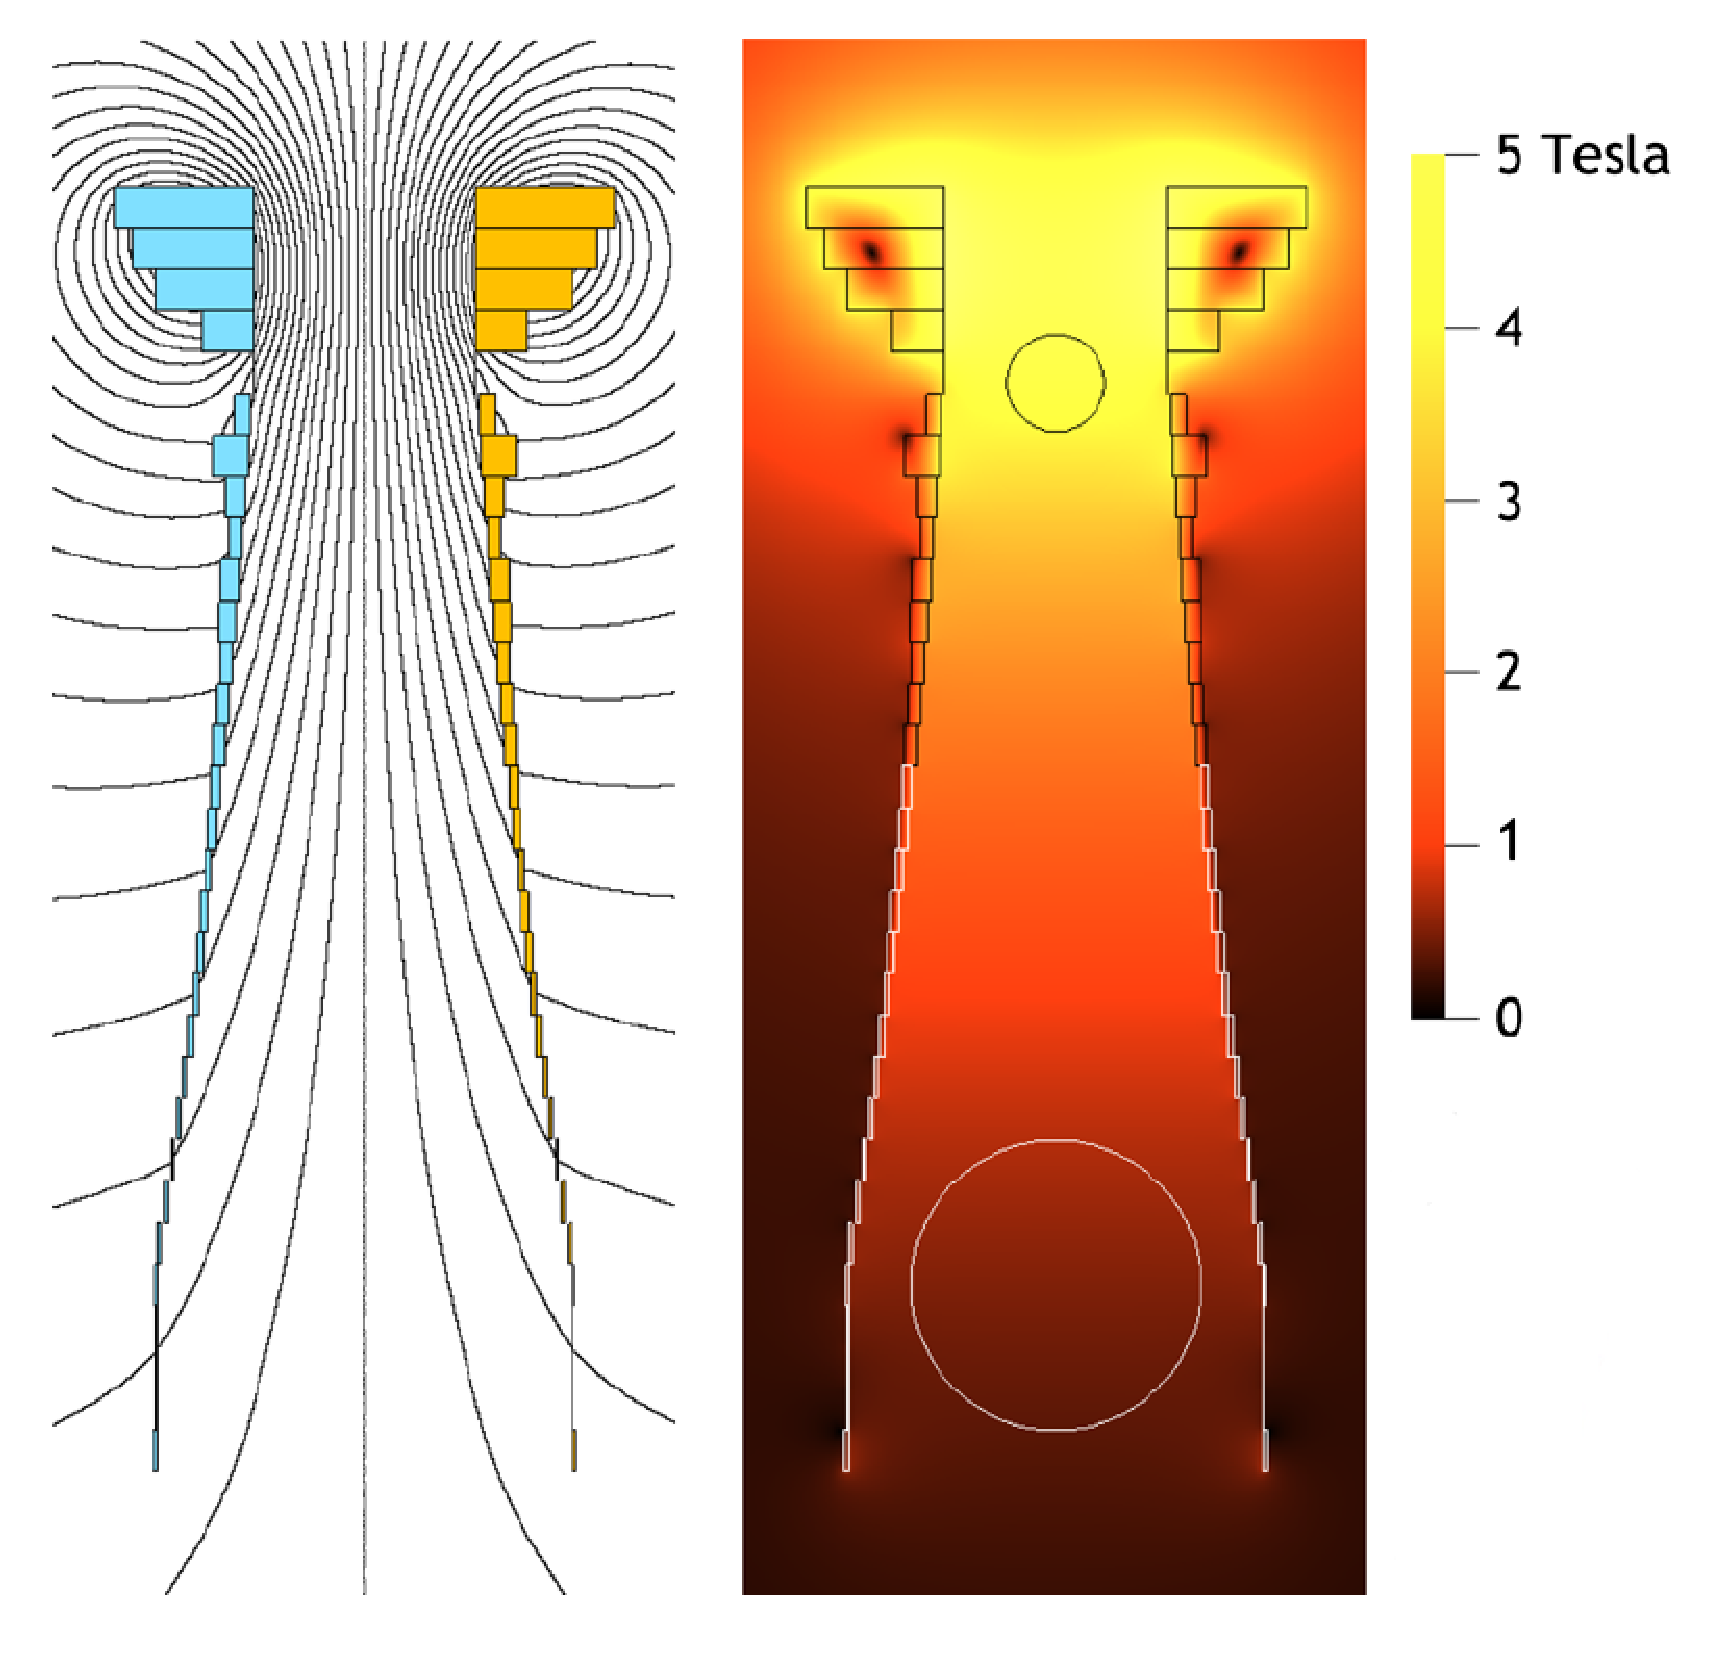
\includegraphics[width=.9\linewidth]{./figs_FFAG_introSlides/./vffag_Mag.eps}

\end{minipage}
} %mbox

\vspace{2ex}

\mbox{
\begin{minipage}{.5\linewidth} 
\centering

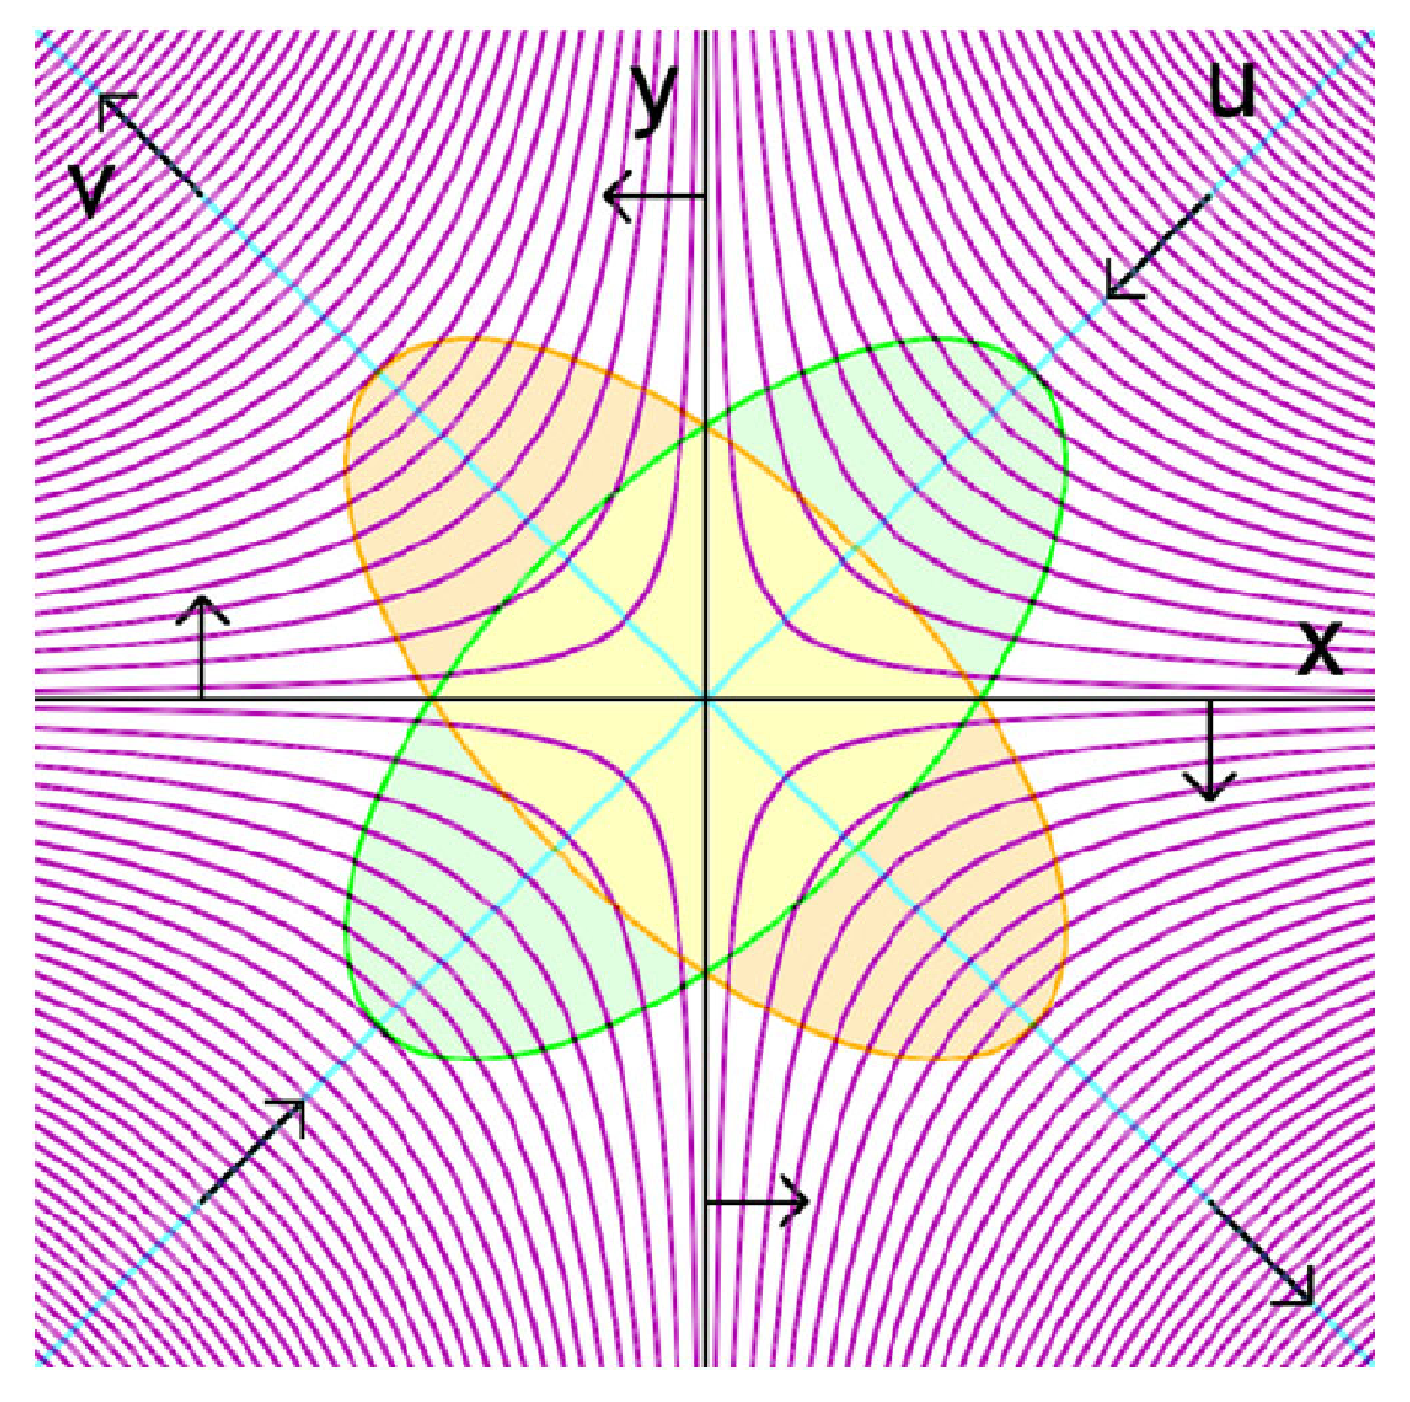
\includegraphics[width=.45\linewidth]{./figs_FFAG_introSlides/./vffag_field.eps}

\end{minipage} \hspace{6ex} 
\begin{minipage}{.4\linewidth} 
\centering

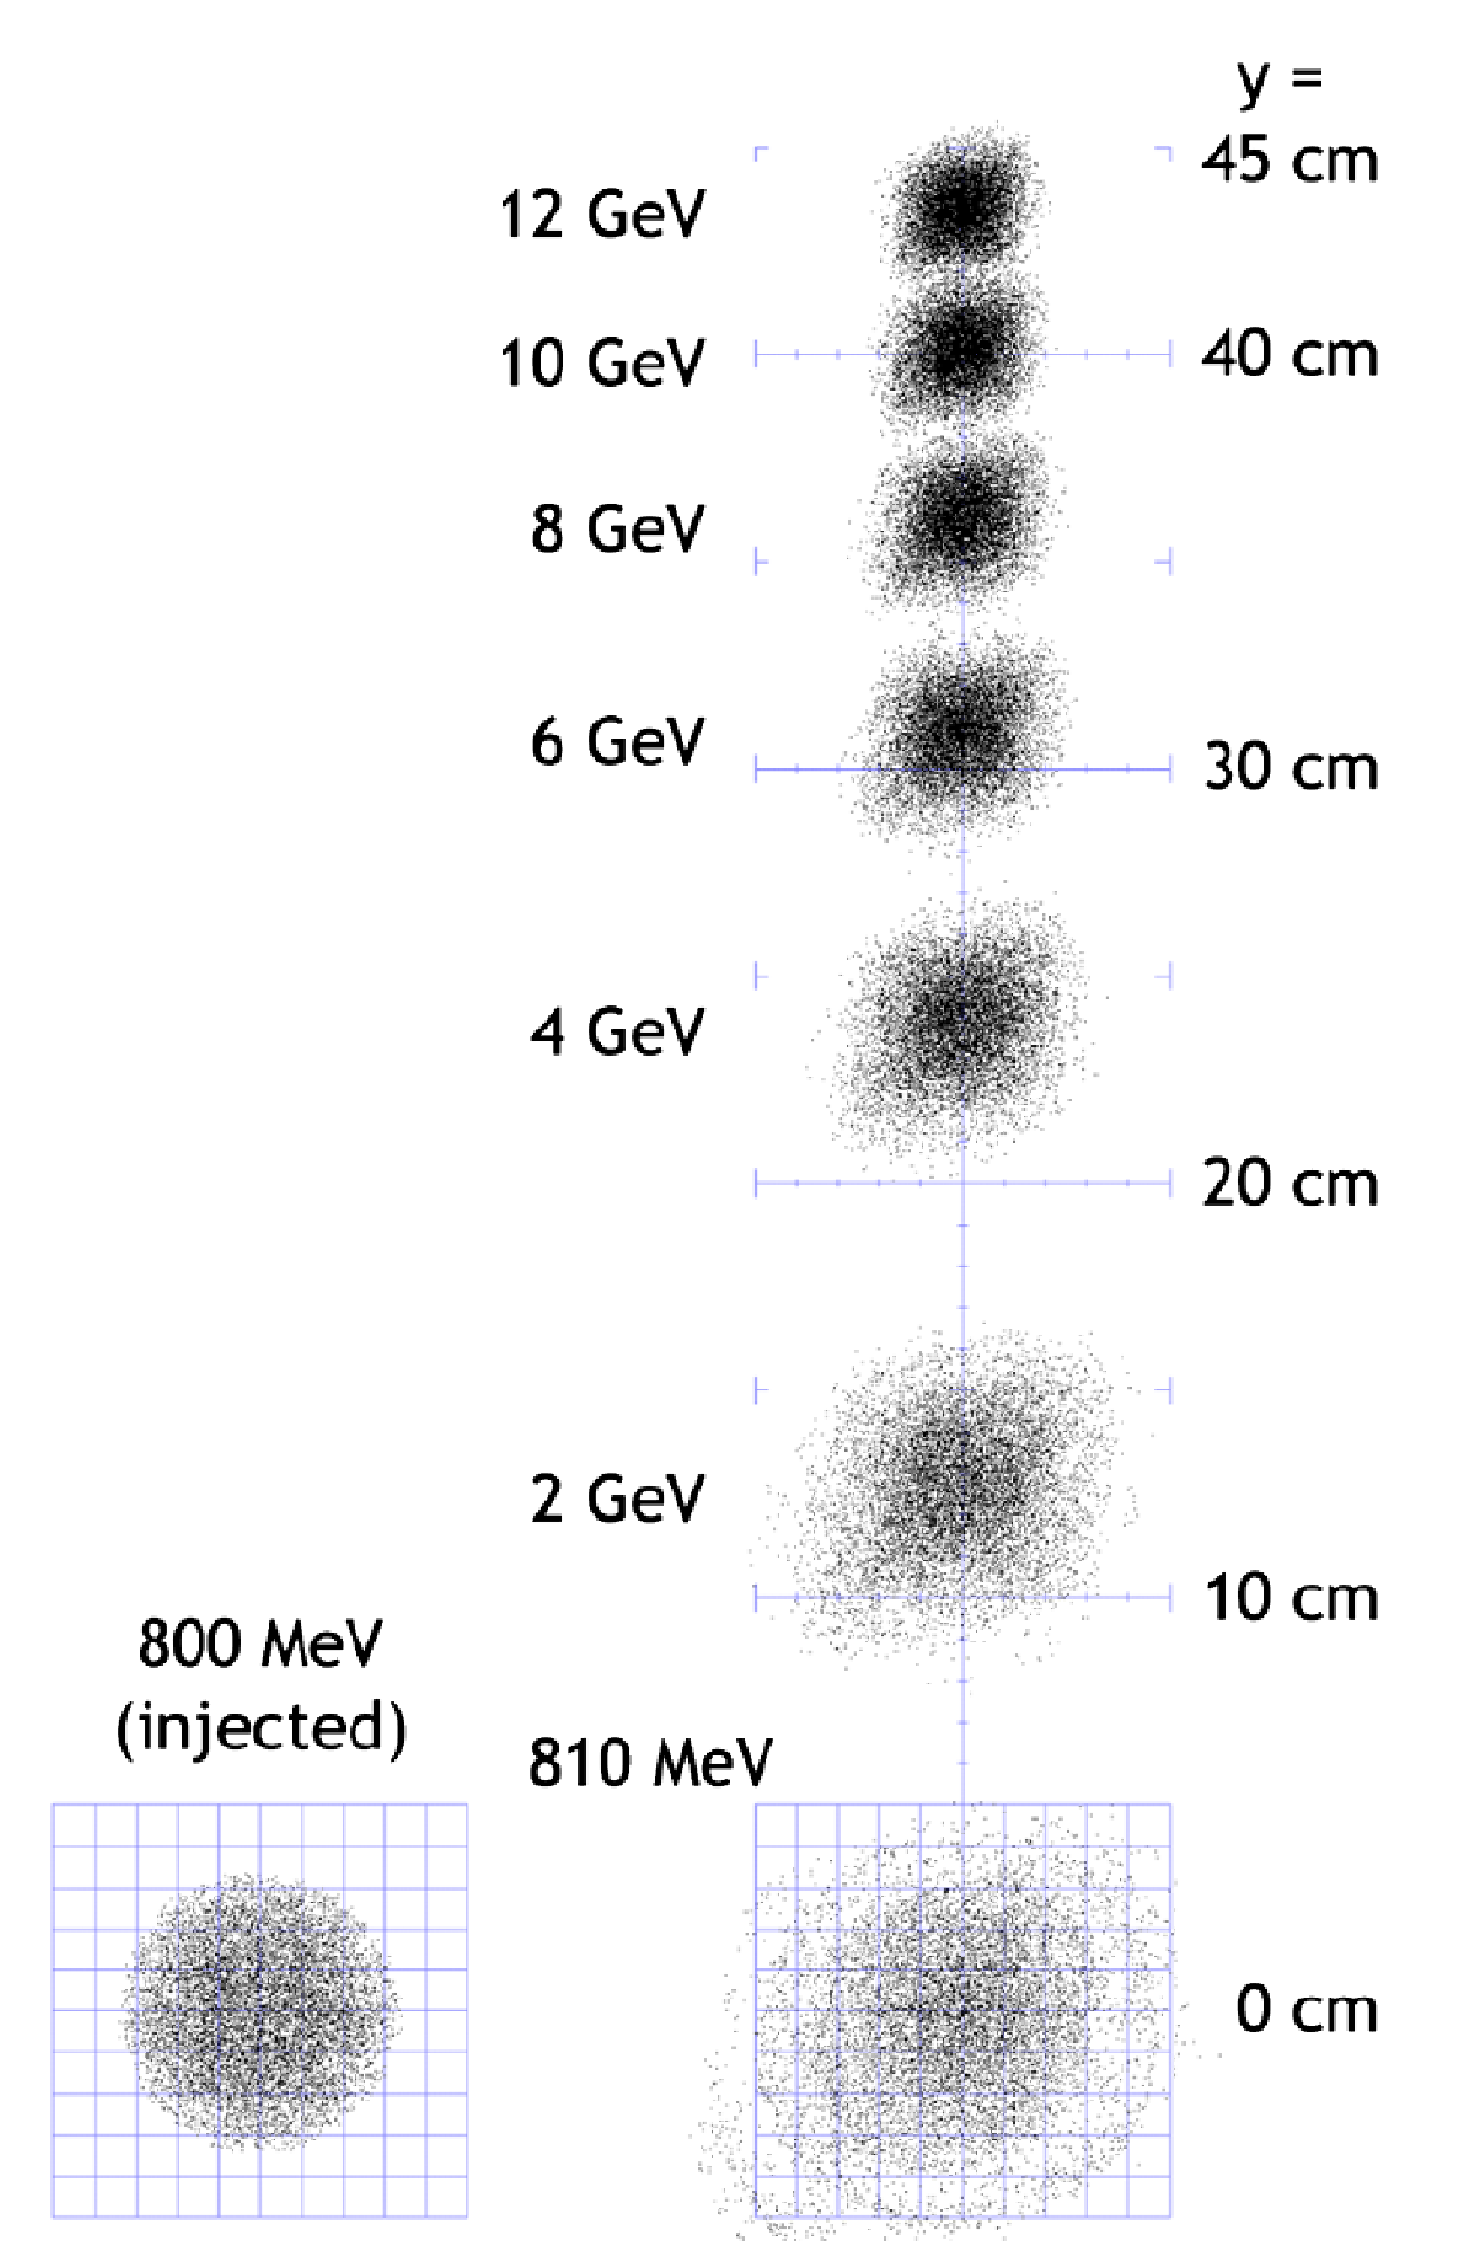
\includegraphics[width=.5\linewidth]{./figs_FFAG_introSlides/./vffag_traj.eps}

\end{minipage}
} %mbox
\end{minipage}



}%fontsize  


\clearpage


\subsection*{\LARGE \bf \blue \nib  A linear FFAG proton-driver design [S. Ruggiero, BNL, 2004]}


\Large

\vspace{-0ex}

\mbox{
\begin{minipage}{0.44\linewidth}

\subsection*{\LARGE \blue  \nid A 3-stage linear FFAG cascade, as a NuFact p-driver  }


  \begin{center}
 \nid Linear  FDF FFAG triplet \\

    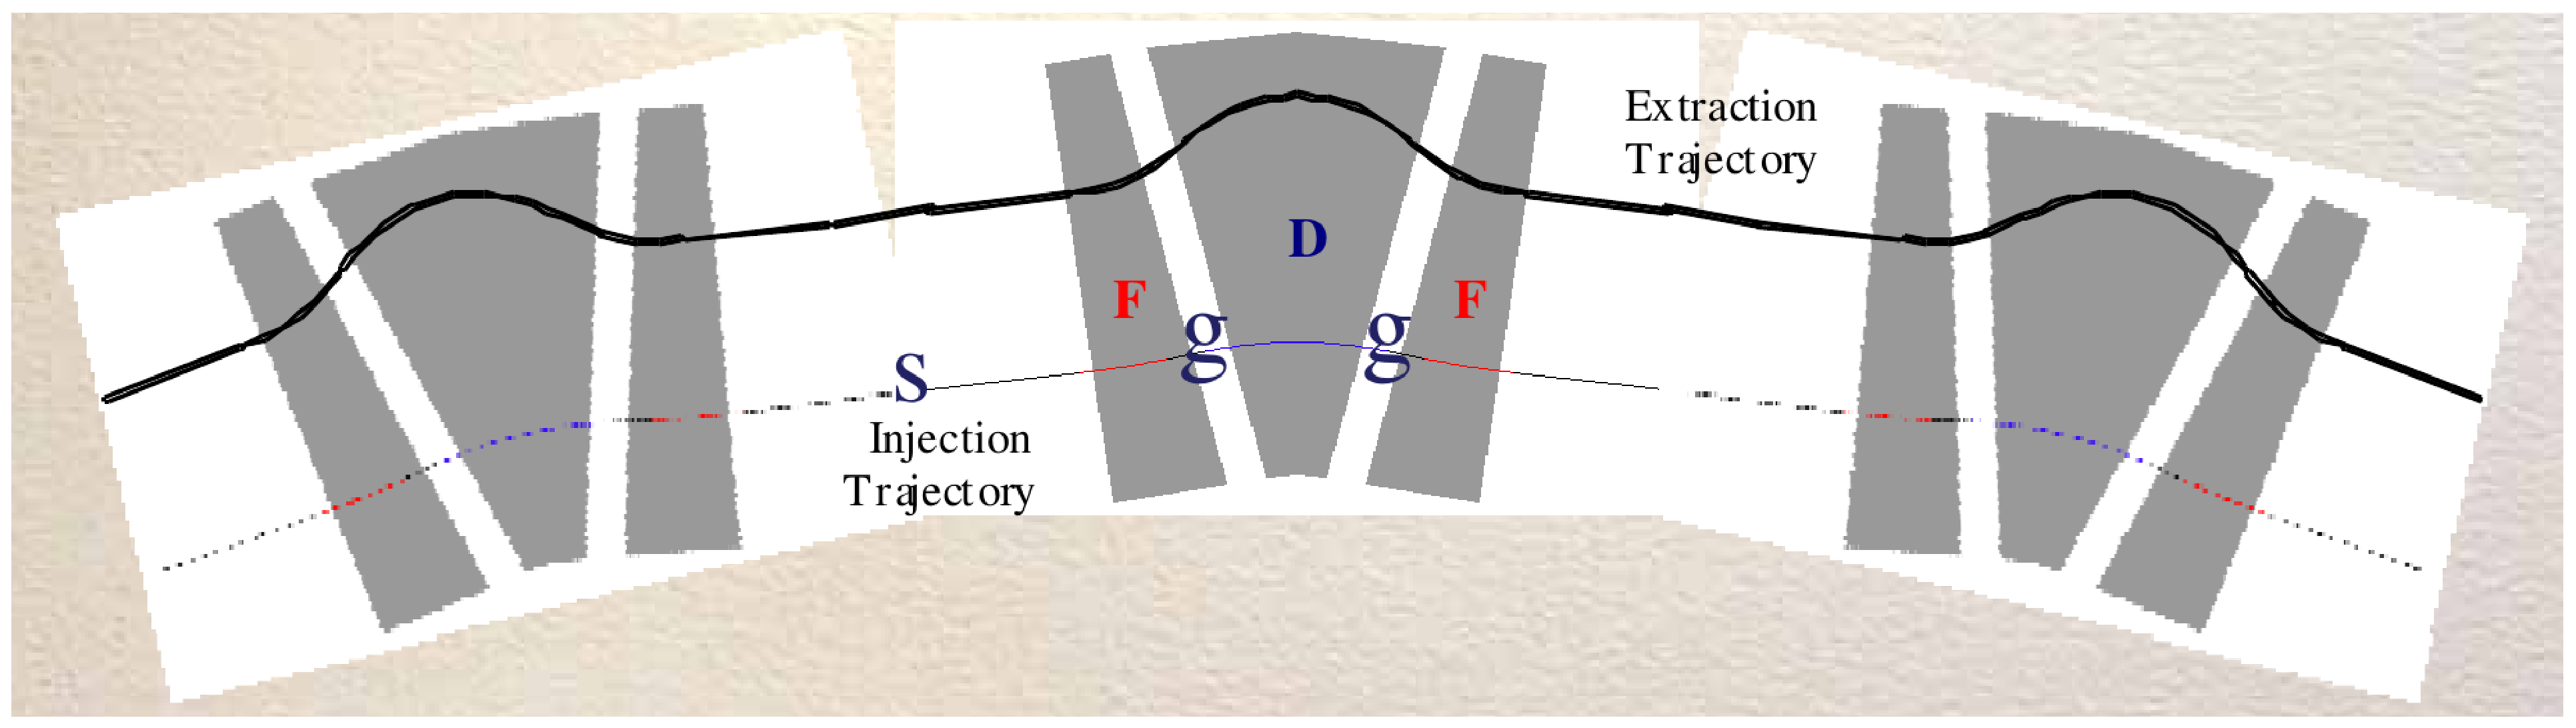
\includegraphics[width=0.85\linewidth]{./figs_FFAG_introSlides/ruggiero_cell.eps} \\[2ex]

    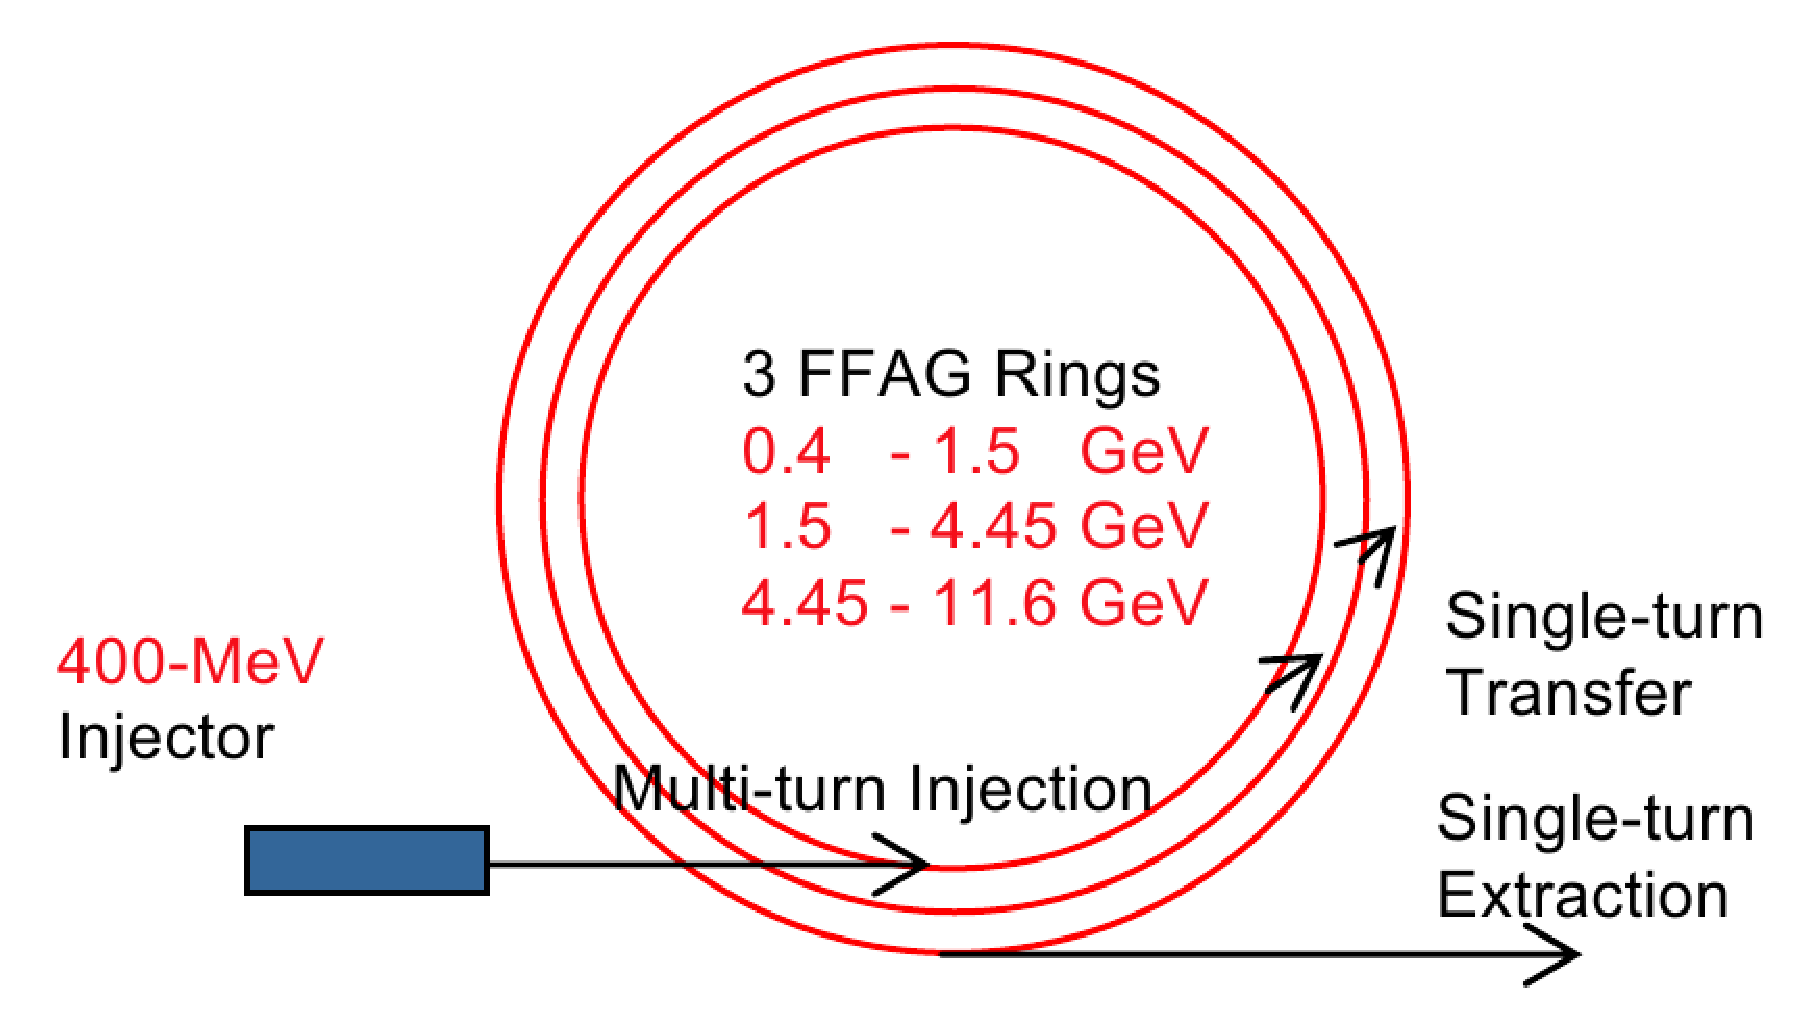
\includegraphics[width=0.95\linewidth]{./figs_FFAG_introSlides/ruggiero_Ring.eps} \\[2ex]


\blue
  \nid Fast resonances crossing~:  \\
$Q_x : 40 \rightarrow 19$, ~ ~ $Q_y : 38 \rightarrow 9$.  \\
    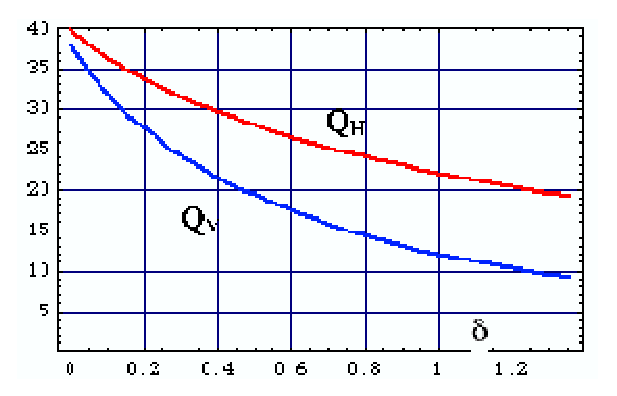
\includegraphics[width=0.5\linewidth]{./figs_FFAG_introSlides/ruggiero_tunes.eps} \\[-1.5ex]
               $(p-p_0)/p_0$
  \end{center}
\end{minipage}%
\begin{minipage}{0.59\linewidth}
\begin{itemize}
\item[\nid] {\bf Neutrino factory p-driver parameters~:
}

\begin{tabular}{lcccc}
\hline 
            &&  \blue  Ring 1     &  Ring 2 & Ring 3       \\
Energy, Inj. &(GeV) &\blue   0.4  &  1.5  &  4.5   \\
\hfill Extr. &(GeV) & \blue  1.5  &  4.5  &  12   \\
\# of turns   && \blue 1800 & 3300 & 3600 \\
cycle time &ms&  \blue 6 & 9 & 10  \\ 
Circumf. &m& \blue 807  &  819  &  831 \\ 
\# cells &&  \blue  136  &  136 & 136  \\
cell length  & (m)  &  \blue 5.9  &  6  &  6.1  \\
h  &&  \blue 136  &  138  &  140  \\
RF freq. &MHz& \blue 36-46 & 46-49.7 & 49.7-50.4   \\ 
E gain / turn & MeV & \blue  0.6 & 0.9 & 2 \\
\hline 
\end{tabular}

~

\blue

\item[\nid] Operation mode variant considered for ring \#1, 
 for $\sim$MW beam power in GeV range~: 

- broad-band, few MHz RF (JPARC style), cycled, 

- repetition rate $>$100~Hz, 


%  \begin{itemize}
%  \item Avoid varying RF frequency
%  \item Proton machines highly non-isochronous
%  \item RF voltage gain varies with transverse position
%  \item Each turn has different integer RF harmonic number
%  \end{itemize}
\black

\item[\nid] Even higher rep. rate. (toward CW)  based on

 - ``harmonic number jump'', 

-  using high frequency fixed-frequency RF.

 Requires cavity with transverse RF voltage profile.  

\black
%\item Refs: (BNL) C-A/AP/208, C-A/AP/218, C-A/AP/219.
\end{itemize}

~

~

\end{minipage} 
}






%\clearpage


\begin{minipage}{1.\linewidth}


\subsection*{\LARGE \blue \nib \bf \blue Pumplet lattice [G. Rees, RAL]}

\LARGE \black
- A \black non-linear, non-scaling \blue type of FFAG, isochronous 

\black
-  A scheme investigated for a  20 GeV, 4~MW proton driver for the neutrino factory 

\medskip

\begin{minipage}{.53\linewidth}
%Recently introduced by G. Rees . \\

%{\Large [Hear G.~Rees' talk]} \\

\vspace{1ex}

 \LARGE \nid The many knobs (field non-linearities) allow isochronism 

\vspace{1ex}

{\bf \large  Lattice for  8 to 20 GeV / 16 turns / 123 cell ring~:  }

\vspace{1ex}

\includegraphics*[width=14cm]{./figs_FFAG_introSlides/FigCellIso.eps}

\vspace{-1mm}

{\normalsize
$B_{bd}(x)= -3.456 - 6.6892 \ x + 9.4032 \ x^2 -     7.6236 \ x^3 + 360.38 \ x^4 +  1677.79\  x^5 $ \\
$B_{BF}(r)= -0.257 + 16.620 \ r + 29.739 \ r^2 +  158.65 \ r^3 + 1812.17 \ r^4 +  7669.53\ r^5 $ \\
$B_{BD}(x)=4.220 - 9.659 \ x - 45.472 \ x^2 - 322.1230 \ x^3 - 5364.309 \ x^4 - 27510.4 \ x^5 $ 
}

~

\fbox{
\begin{minipage}{.99\linewidth}
{\bf \blue  Allows insertion straights } - advantages~: 

\Large 

 1. easier injection and extraction,

 2. space for beam loss collimators,

 3. RF gallery extending only above the insertions, not above the whole ring,

 4. 4-cell cavities usable, thus reducing, by a factor of four, the
     total number of rf systems.
\end{minipage}
}

\end{minipage}
\begin{minipage}{.5\linewidth}

\vspace{-0ex}

 \begin{center}



 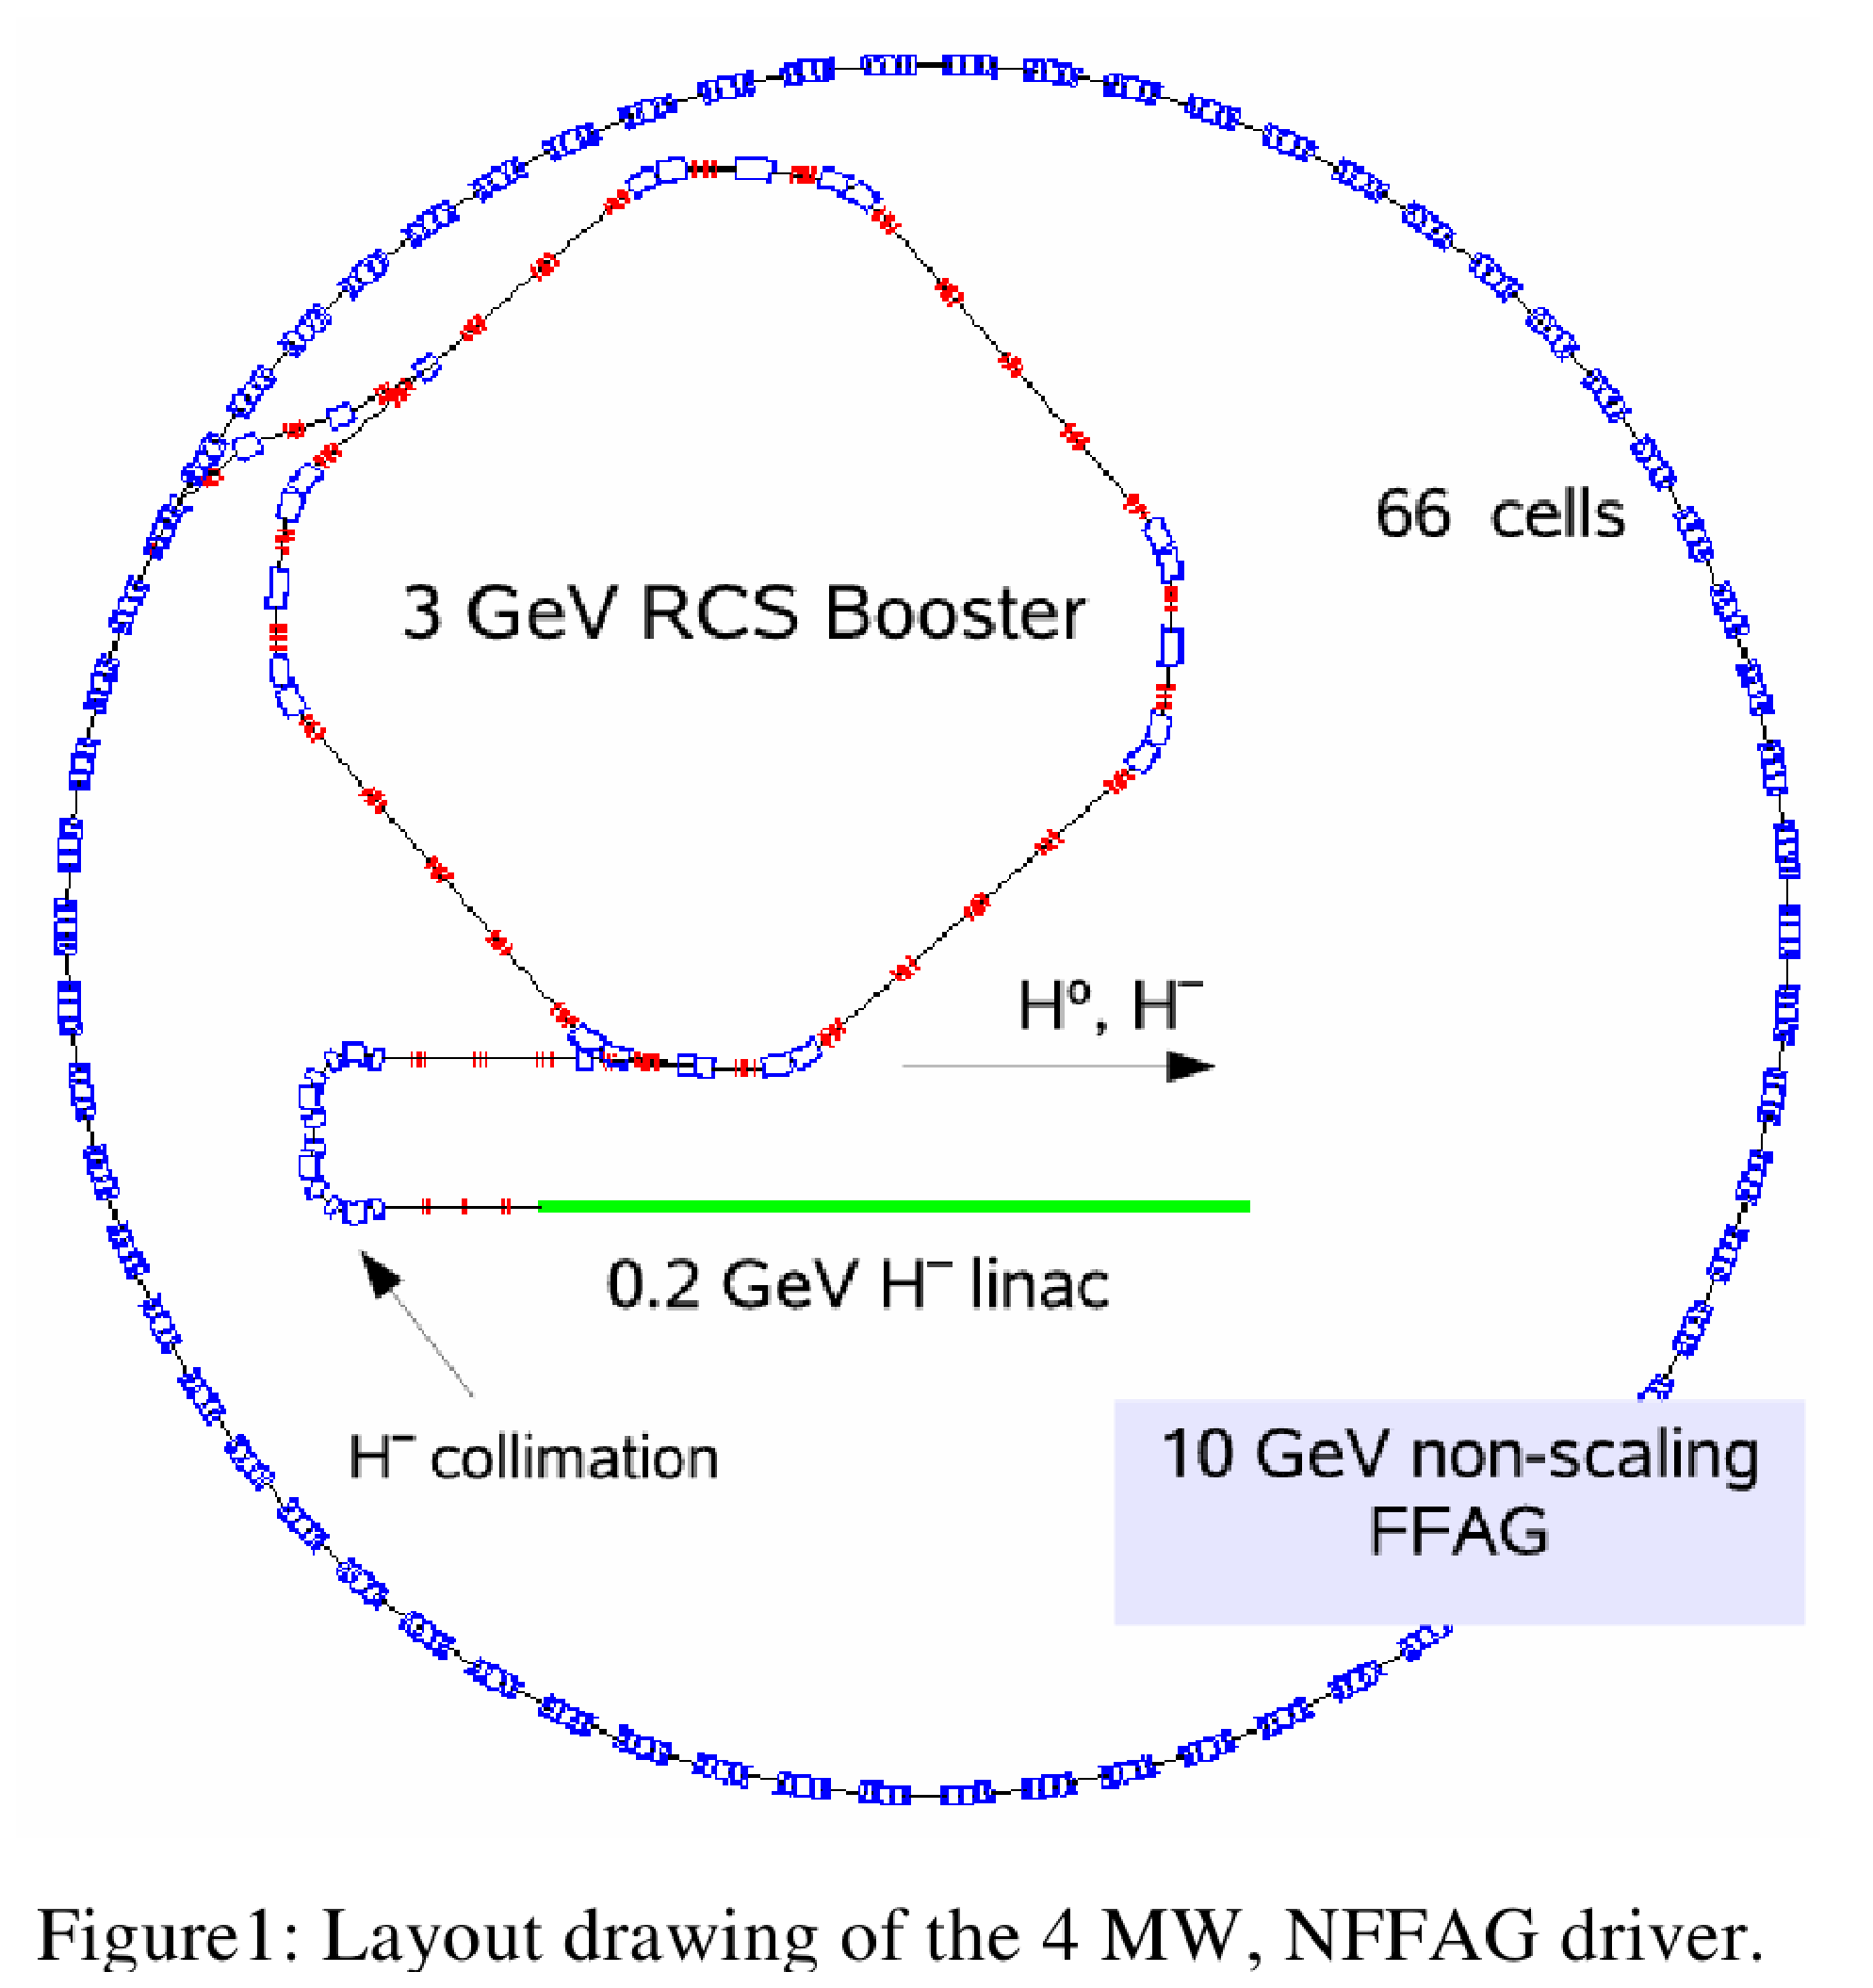
\includegraphics[width=.45\linewidth]{./figs_FFAG_introSlides/pumpletRing.eps}
% 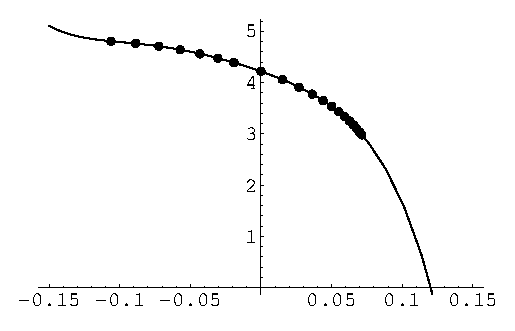
\includegraphics[width=6cm,width=5cm]{./figs_FFAG_introSlides/BDField.eps}

~

\nid Field profile in  BF and BD : 

\mbox{
 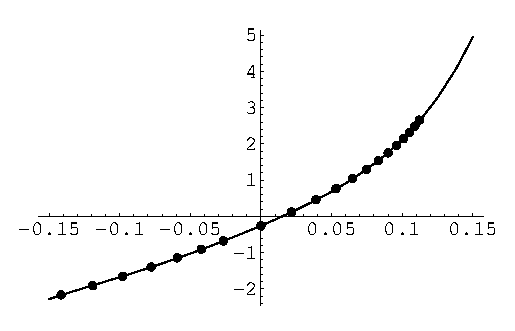
\includegraphics[width=5cm]{./figs_FFAG_introSlides/bfField.eps}  ~ ~ 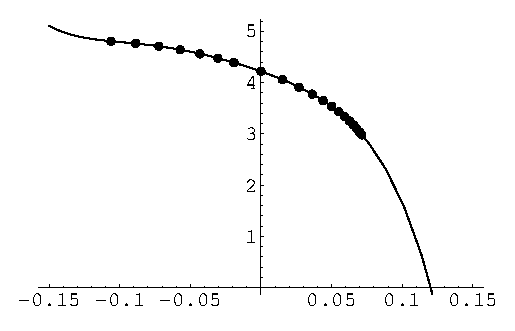
\includegraphics[width=5cm]{./figs_FFAG_introSlides/BDField.eps}
}

~~~~~



{\Large 
\blue  
\nid Beam trajectory in the tune diagram : 
}

 \includegraphics*[width=10.0cm,height=5cm]{./figs_FFAG_introSlides/Tunes_co_muon.eps}

 \end{center}


\end{minipage}


\end{minipage}










\clearpage

\subsection*{\LARGE \blue \nib \bf \blue Toward CW [C. Johnstone, FNAL]}

\LARGE

\vspace{-1ex}

\medskip

\subsubsection*{\LARGE \black Quasi-isochronous optics, } 

\vspace{-1ex}

\nid based on SC dipoles and featuring

- alternating-gradient with non-linear radial field profile 

-  optimized magnet-edge contour


\medskip

\blue 

\nid Allows near-crest (serpentine) acceleration, based on  SCRF

\black

\vspace{2ex}

\fbox{
\begin{minipage}{.99\linewidth}

\centering
%\blue 

\nid Principle 6-cell lattice used for numerical beam dynamics studies~:

\medskip 


\mbox{
\begin{minipage}{.55\linewidth}

\medskip

\blue 0.33 to 1~GeV at a rate of 10$\sim$20~MV/turn

~

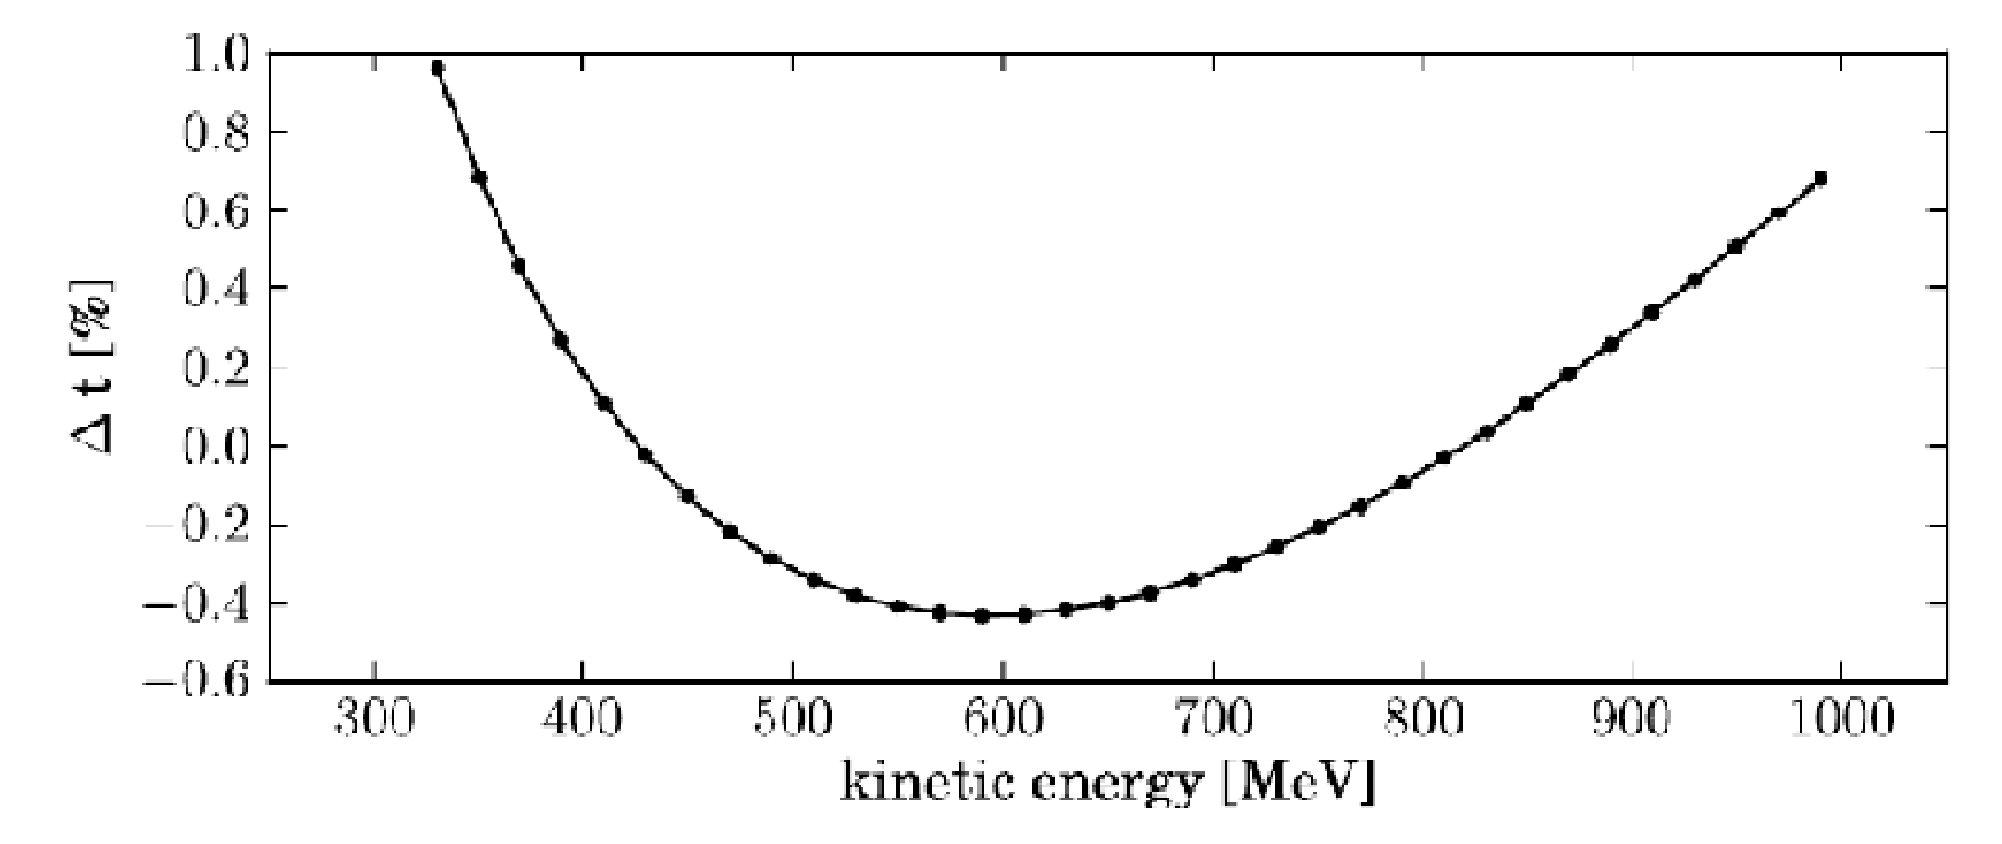
\includegraphics[width=.9\linewidth]{./figs_FFAG_introSlides/carolsTOF.eps} 

\end{minipage}  ~ 
\begin{minipage}{.55\linewidth}

~ \hspace{5ex} ~
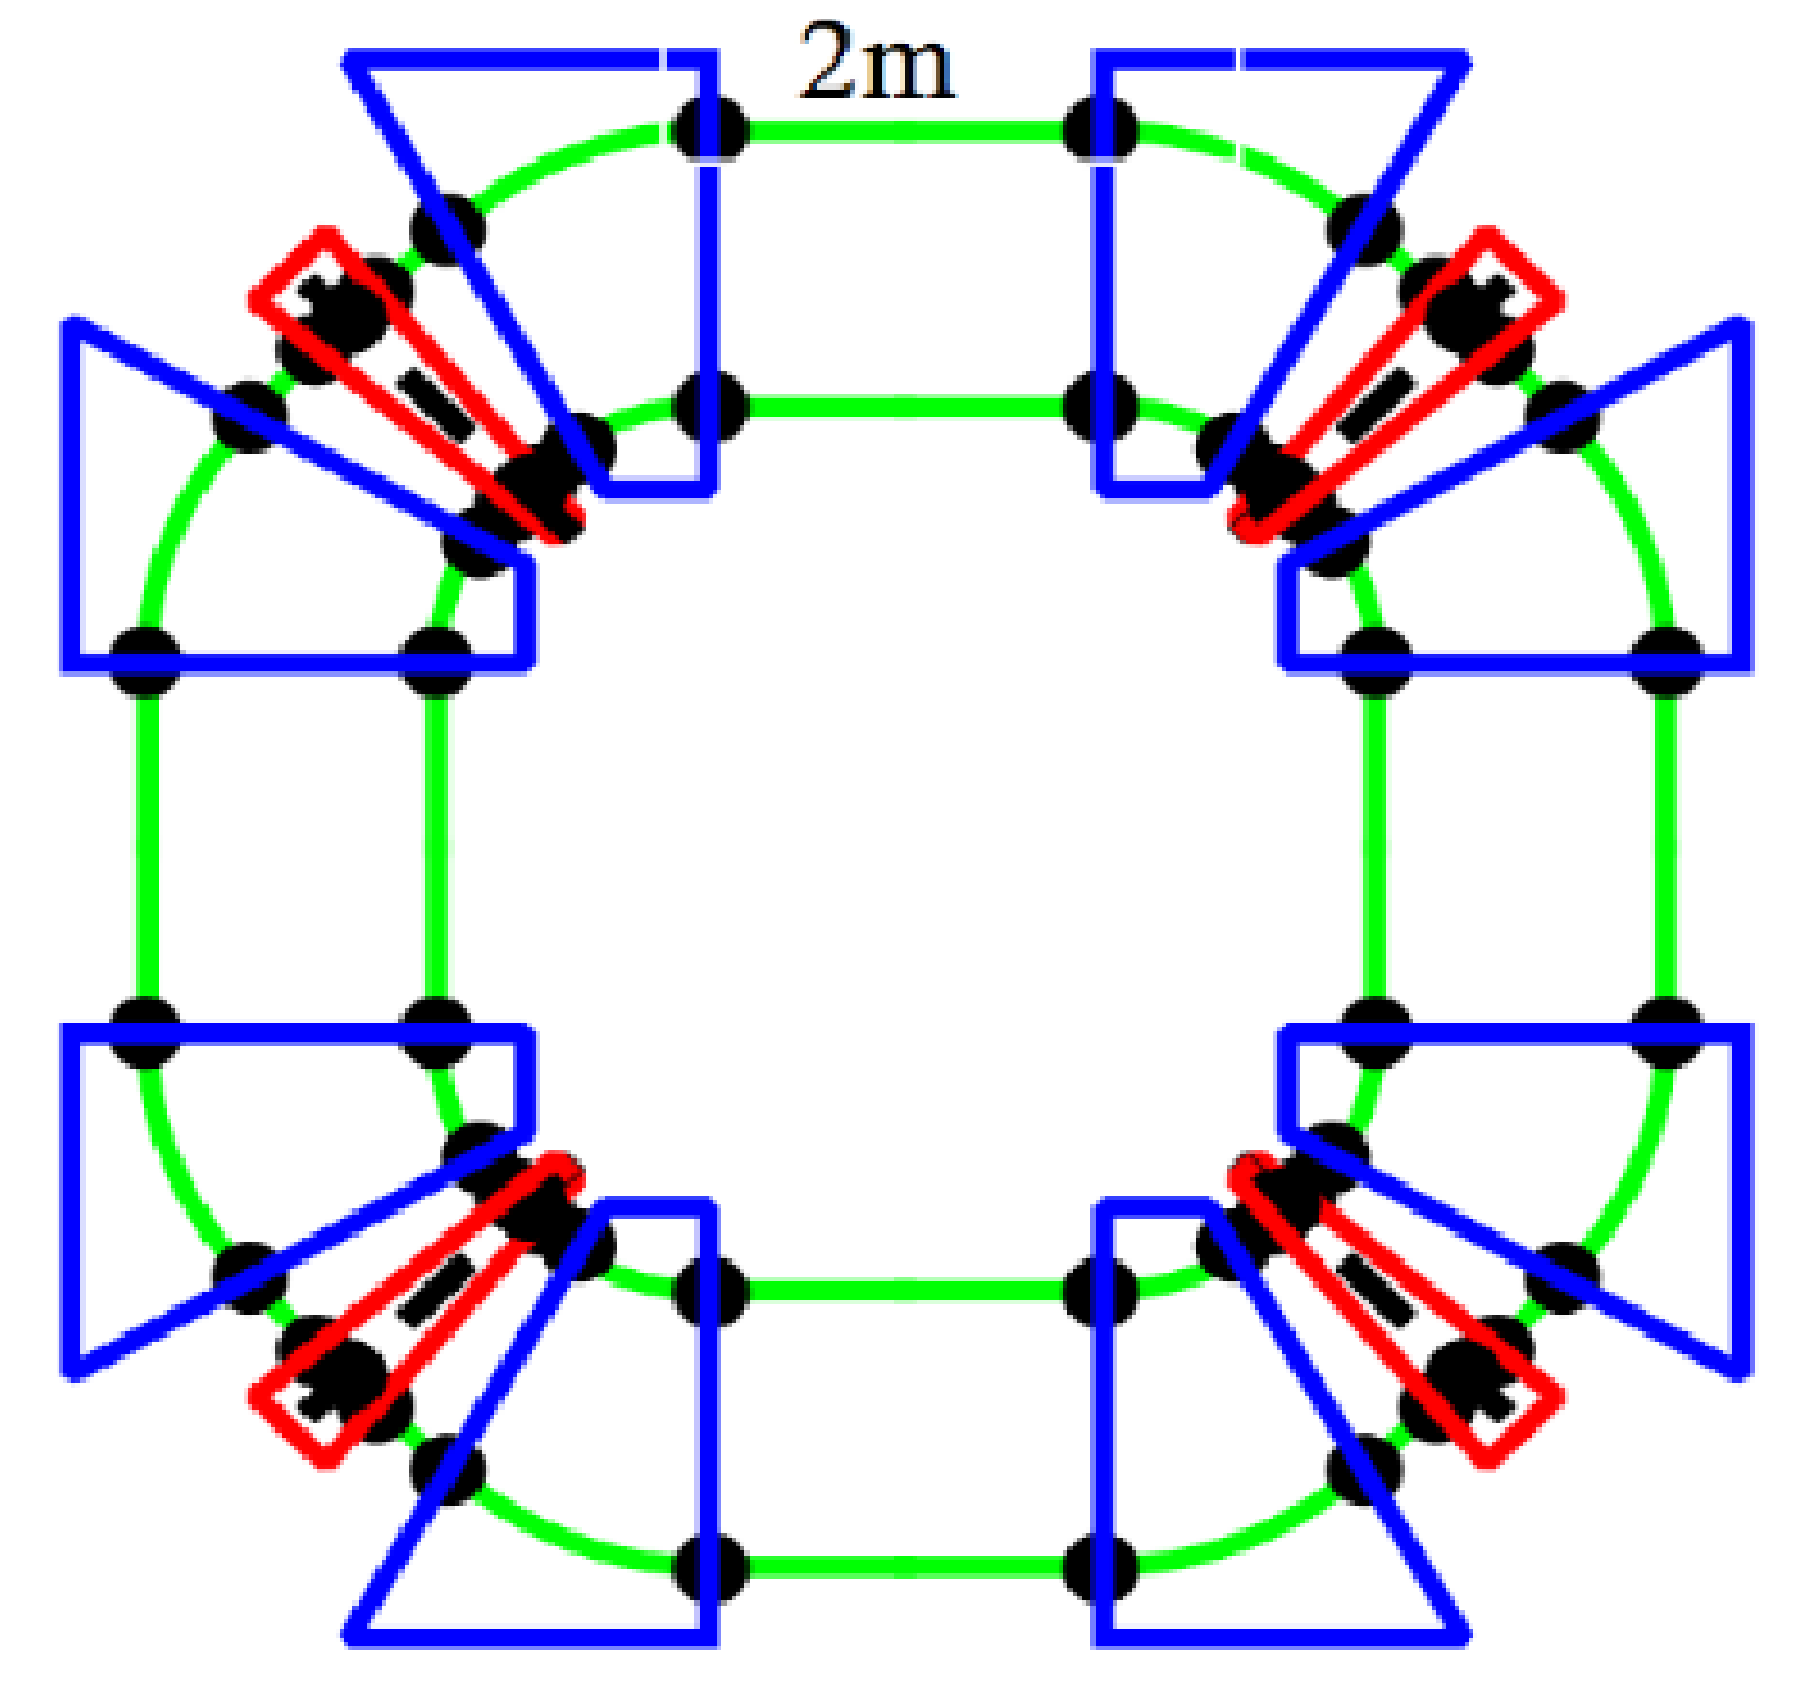
\includegraphics[width=.6\linewidth]{./figs_FFAG_introSlides/carolsRing.eps}  

\end{minipage}
}

\end{minipage}

}

\bigskip

\black
\nid Numerical beam dynamics studies show 

\blue
\medskip 

- large transverse dynamical acceptance 

- currents in  20~mA range with no transverse beam growth doable  (OPAL simulations)




\clearpage

\LARGE

\black
\subsubsection*{\LARGE \nib \bf Serpentine acceleration  in scaling lattice, FFFFAG [E. Yamakawa et al., KURRI]}



\blue
\nid  The lattice $\gamma_{\rm tr}=\sqrt{1+K}$ is set to be in the acceleration range~: 
beam $\gamma$ is accelerated in transition region, time of flight is parabolic 

\smallskip
\black
\nid This allows using fixed RF-frequency acceleration in \blue variable $\beta=v/c$ regime \black 

- i.e., case of non-relativistic beam, suitable for proton acceleration.

\rm \black

~


\begin{minipage}{.38\linewidth}


\blue

\nid \bf Experimental demonstration performed with an electron prototype (Japan, 2012): 

\black

~

- small e-beam ring

- 160~keV $\rightarrow$ 8~MeV

- F-D-F scaling triplet lattice at transition gamma
 (764~keV) 

- RF freq. 75~MHz (h=1), 750~kV/gap
\end{minipage}\hspace{3ex}
\begin{minipage}{.01\linewidth}
\rule{0.1mm}{140mm}
\end{minipage}\hspace{0ex}
\begin{minipage}{.51\linewidth}

\centering

\blue
\nid \bf An ADS equivalent has been designed

(NIM A 716 (2013))

\black

~

\rm

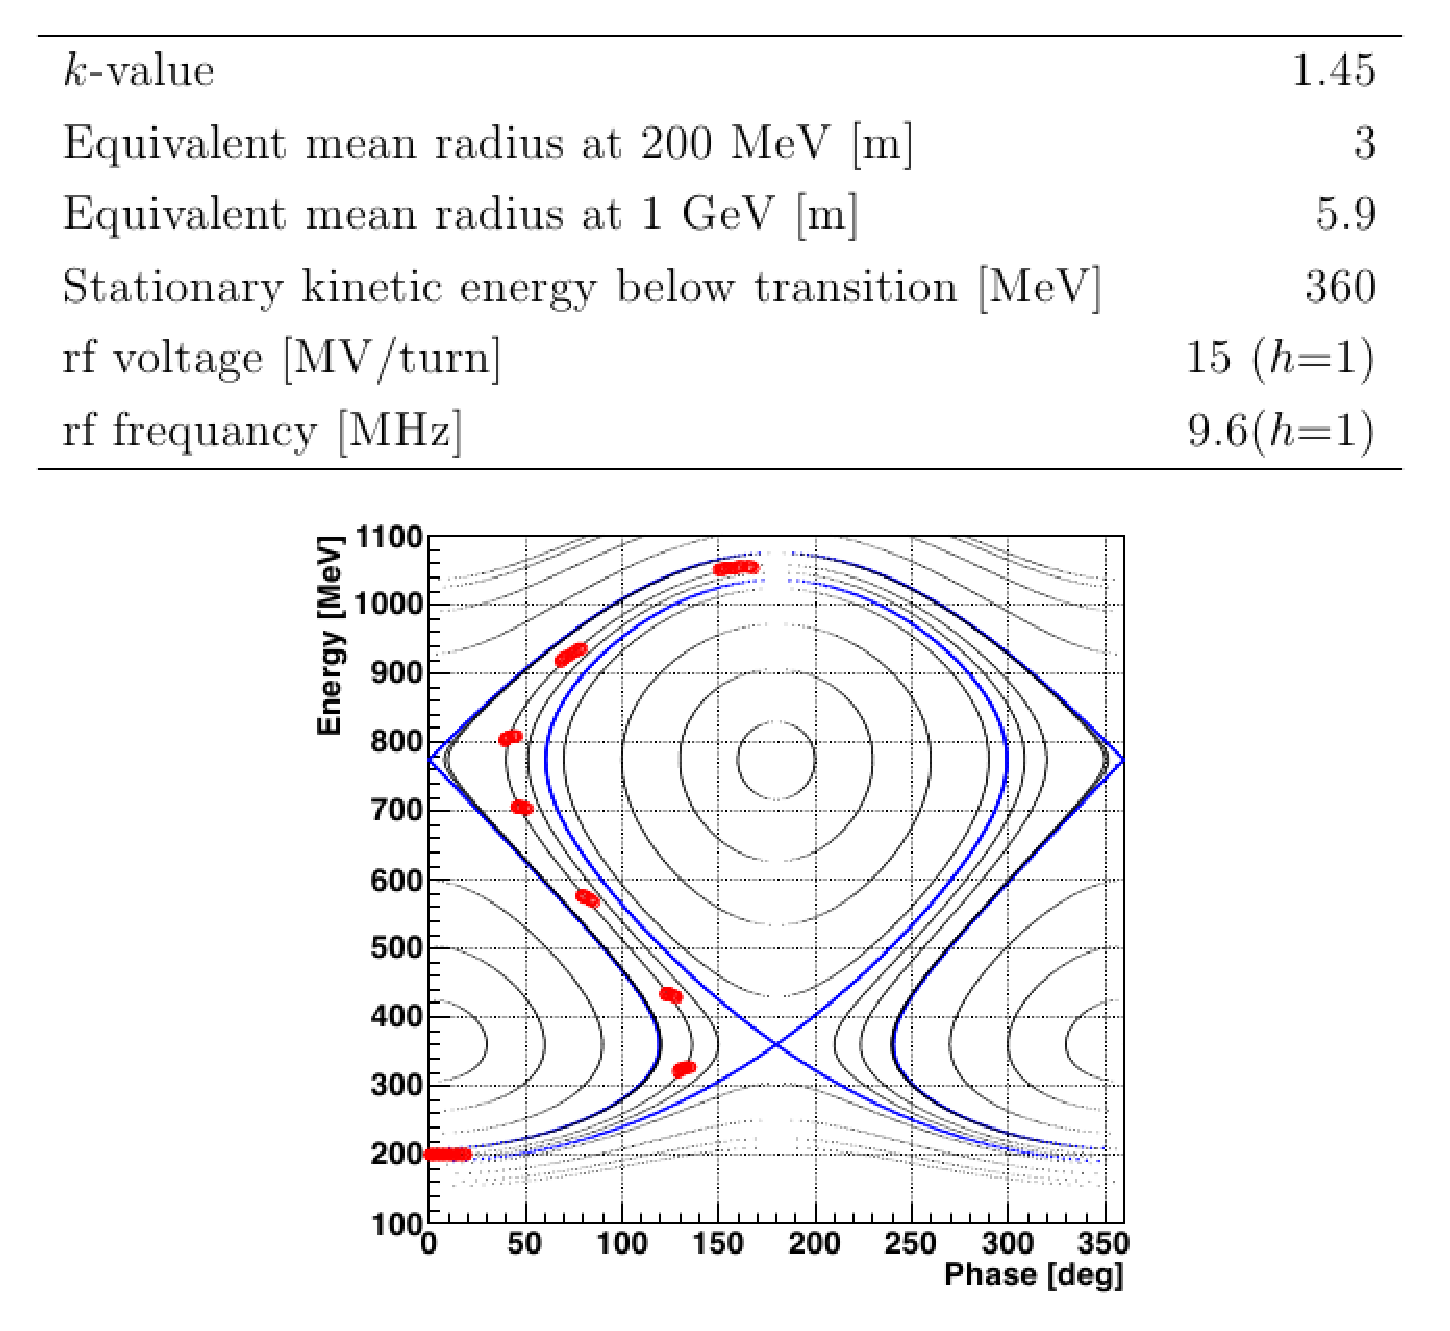
\includegraphics[width=1.\linewidth]{./figs_FFAG_introSlides/serpentineEmi.eps}
\end{minipage}

\black






\clearpage 

{\fontsize{18}{34} \selectfont

\bf 

\section*{\Huge And today ...}

~


\centerline{More going on !}



~


\centerline{\Huge \blue \fbox{THANK YOU FOR YOUR ATTENTION}}
}

~


\centerline{
 \hspace{0mm}  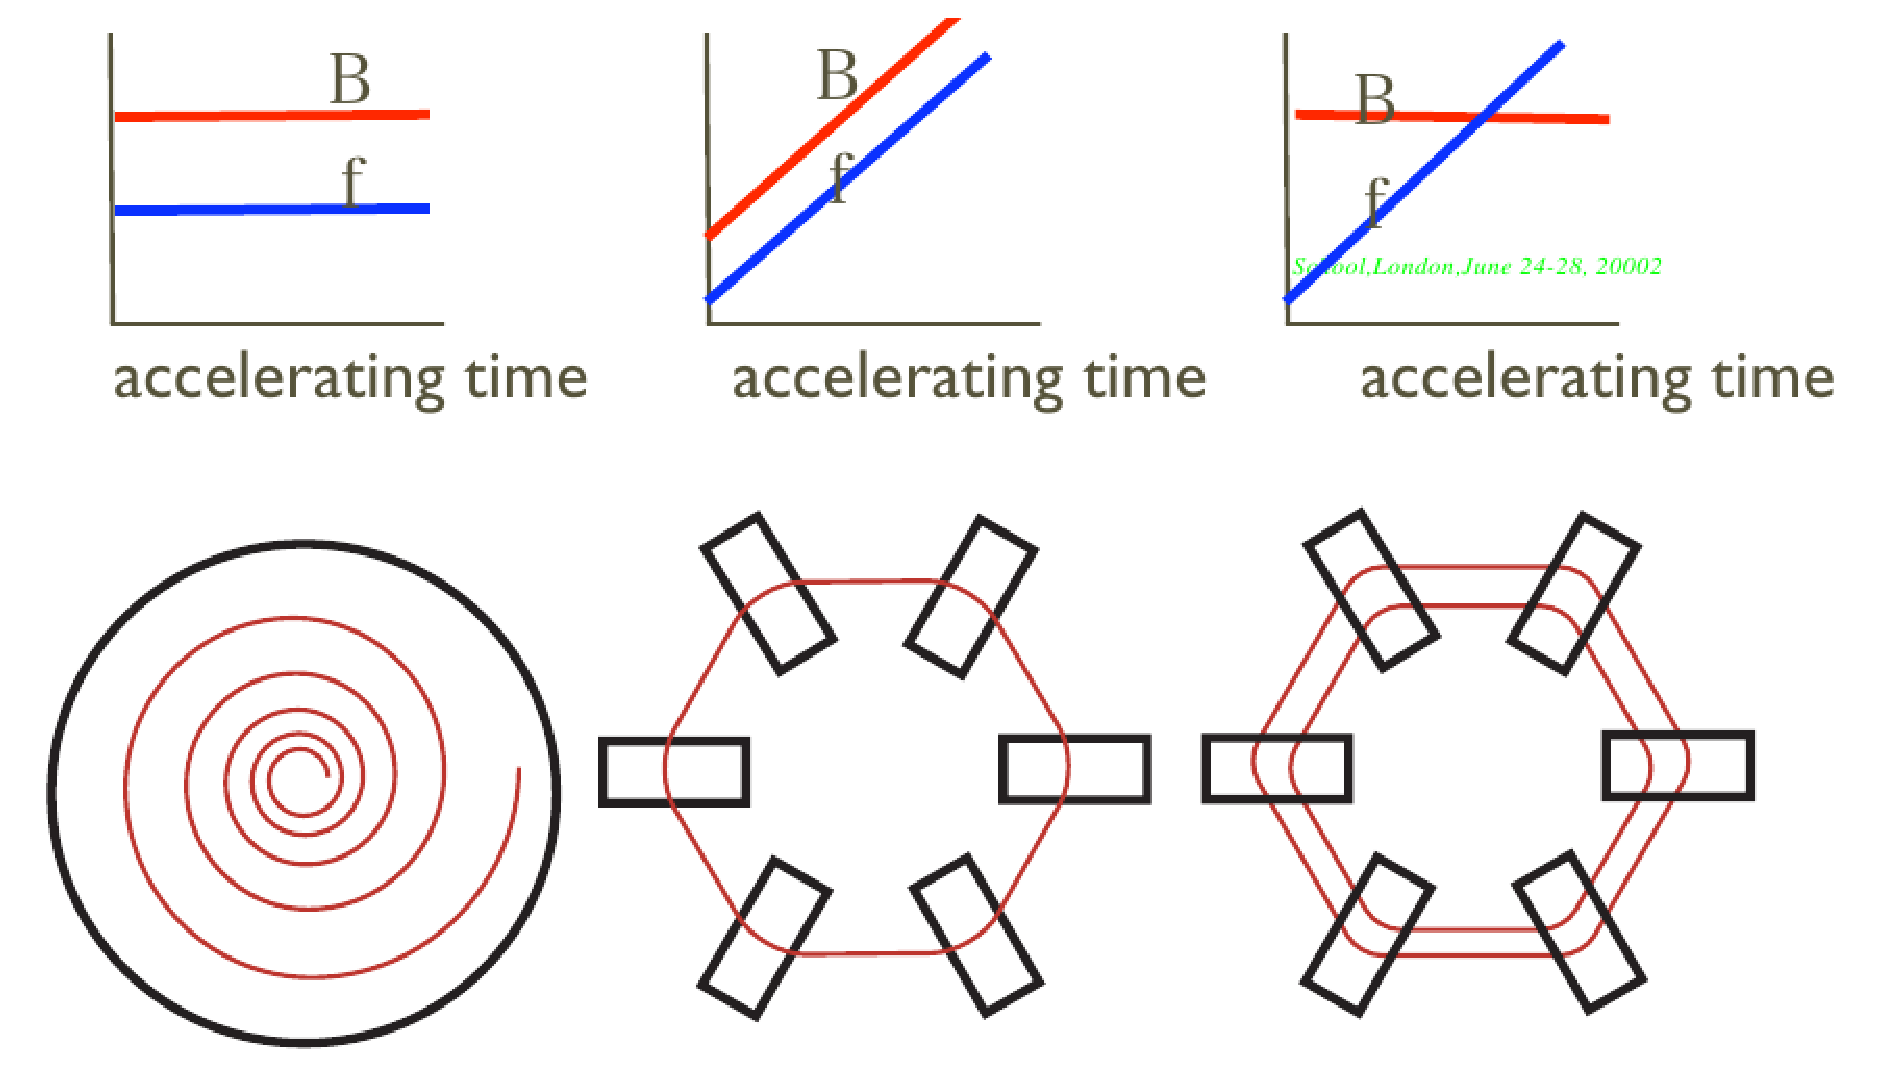
\includegraphics[bbllx=14,bblly=140,bburx=781,bbury=568,width=15cm]{./figs_FFAG_introSlides/page3R.eps}
}


\end{document} 









\subsection*{\Large  \nib   The first model, radial sector FFAG, ``MARK~I''}

\large   

\nid Main features~:  fixed field ring, $B=B_0 (r/r_0)^K \, \mathcal{F}(\theta) \ \ \Rightarrow$ strong focusing, zero chromaticity. 

\smallskip

\nid Objectives~:  confirm theoretical predictions~; study FFAG  properties~: optics, injection, test RF programs~; 
effects of misalignments~; effects  of resonances. 


\begin{minipage}[b]{.26\linewidth}

%\hspace{-7mm}  \includegraphics*[bbllx=40,bblly=50,bburx=440,bbury=350,width=7.5cm]{./figs_FFAG_introSlides/ring1Photo.eps}

\centering

\includegraphics*[bbllx=90,bblly=130,bburx=760,bbury=440,width=.9\linewidth]{./figs_FFAG_introSlides/ring1MagPhoto.eps} 

\vspace{-0mm}


F magnet, $B>0$, H-focusing

scaling gap g$\propto$r

~

\includegraphics*[width=1.1\linewidth]{./figs_FFAG_introSlides/mark1.eps}


~~~~~~~~~~~~~

\includegraphics*[bbllx=34,bblly=70,bburx=245,bbury=220,width=7cm]{./figs_FFAG_introSlides/ring1Draw.eps}


\end{minipage}\hspace{1mm}
\begin{minipage}[b]{.65\linewidth}
\large

~

{\blue    
First operation March 1956, U of Michigan. }

\vspace{-5mm}
  \begin{center}
   \begin{tabular}{llccc}
\multicolumn{4}{c}{\bf PARAMETERS}    &       \bf   \\[2mm]
&$E_{inj} - E_{max}$&\it keV&    25 - 400      & \bigg\{\raisebox{1ex}[0mm][0mm]{\it small size, easy to build ~~ ~ ~~ ~ ~~}  \\
    &  &   &  &\raisebox{2ex}[0mm][0mm]{\it field not too low, ms lifetime }   \\
      & orbit radius  ($\mathcal{C}/2\pi$) &\it m&0.34 - 0.50& \normalsize \bf SPIRALING ORBIT    \\
\\[-2ex]
\multicolumn{2}{l}{\it \underline{Optics}} & \multicolumn{3}{l}{\bf strong focusing, ~ scaling }   \\
      & lattice cell   &     &$\mathbf{ \frac{D}{2}F\frac{D}{2}}$&   \\
      & number of cells& &       8           &  \it 16 magnets, 4.41 deg. drifts\\
      &field index $K$&  &      3.36         &  \it $g/r=$Cst  \& coil windings         \\
      &$\nu_r~/~\nu_z$&  &   2.2-3 ~/~ 1-3   & \bigg\{  \raisebox{1ex}[0mm][0mm]{\it ~ varying K, resp. $B_F/B_D$~~}  \\
      &            &     &              &\raisebox{2ex}[0mm][0mm]{\it varies  mostly  $\nu_r$, resp. $\nu_z$}\\[-2ex]
      &  $\gamma_t$ &  &     $\approx 2$  &       \it  $\sqrt{1+K}$  \\
\\[-2ex]
\multicolumn{2}{l}{\it \underline{Magnet}}&  \multicolumn{2}{l}{\bf radial sector} & \it  $B=B_0 (r/r_0)^K \, \mathcal{F}(\theta)$ \\
&$\theta_F,~ \theta_{D}$&\it deg&    25.74, ~ 10.44 &  \it sector angles        \\ 
      &  $r_{F,D}/\rho$& &     2.85, ~ 2.59  &   \it at center of F, D magnets       \\
      &   gap      &\it cm  &     6 - 4          &   \it $g/r=$Cst  \\     \\
\\[-3ex]
\multicolumn{2}{l}{\it  \underline{Injection}}&  \multicolumn{3}{l}{\bf continuous or pulsed }  \\
\\[-1.5ex]
\multicolumn{2}{l}{\it  \underline{Acceleration}}& \multicolumn{3}{l}{\blue MARK I started with betatron yoke...   }         \\
      & swing  &\it  Gauss &   40 - 150   &  \\
      & rep. rate&\it Hz&      \textsf{a few 10's}          &       \\
\multicolumn{2}{l}{\it }& \multicolumn{2}{c}{\blue ... equipped with RF system, later   }  &  \it split system,  \\
      & freq. swing&\it MHz &  10\textsf{~in}~ [35,~75]~\textsf{MHz}  &  \it  for  RF stacking expts\\
      & gap voltage&\it V  &        50         &  \\
%      &cycle rep. rate&\it kHz&      \textsf{a few}          &  \it to cope with lifetime    
   \end{tabular}
  \end{center}

~~~~~~~~~~~~~

\end{minipage}


